\documentclass[fleqn, final]{../styles/unmphythesis}
\usepackage{../styles/qxd}
\renewcommand{\thechapter}{2}
%\newcommand{\thechapter}{1}

\makeindex
\begin{document}

%<*waveguideinterface>

\chapter{Atom-waveguide interface}\label{chap:waveguideinterfaces}
\section{Introduction}
In this chapter, we review the semiclassical theory of the interaction of the electromagnetic field (treated classically) with an atom trapped near the surface of a waveguide.  We consider the case that only one atom is trapped nearby a waveguide. As will be discussed later, in the dispersive regime, the interaction from many atoms can be treated as a sum of the interactions from all individual atoms. To be specific, for this chapter, we consider the following scenario: a laser beam propagates through a waveguide along the $ z $ direction; an alkali atom (cesium, for example) is trapped at $ \mathbf{r}_{\rm atom} =\mathbf{r}'$ in the evanescent field of the waveguide~\footnote{We will use the prime ($ ' $) notation to indicate the position of a photon emitter.} and responds to the guided optical field dispersively. In the dynamics, we consider dispersive phase shift of the light and ignore intensity attenuation in photon detections. Effectively, the presence of the atom outside of the waveguide changes the index of refraction\index{index of refraction} of the waveguide. 
The dispersive light shift applies when the saturation parameter is small,
\begin{align}
s=\frac{\Omega^2/4}{\Delta^2+\Gamma^2/4}\ll 1,
\end{align}
where $ \Omega $ is the Rabi frequency, $ \Gamma $ is the spontaneous emission rate of the atom, and $ \Delta=\omega_0-\omega_{eg} $ is the probe detuning from the atomic resonance frequency $ \omega_{eg} $ as a two-level system with the probe's frequency set to be $ \omega_0 $. 

\begin{figure}
\centering\makebox[\textwidth]{
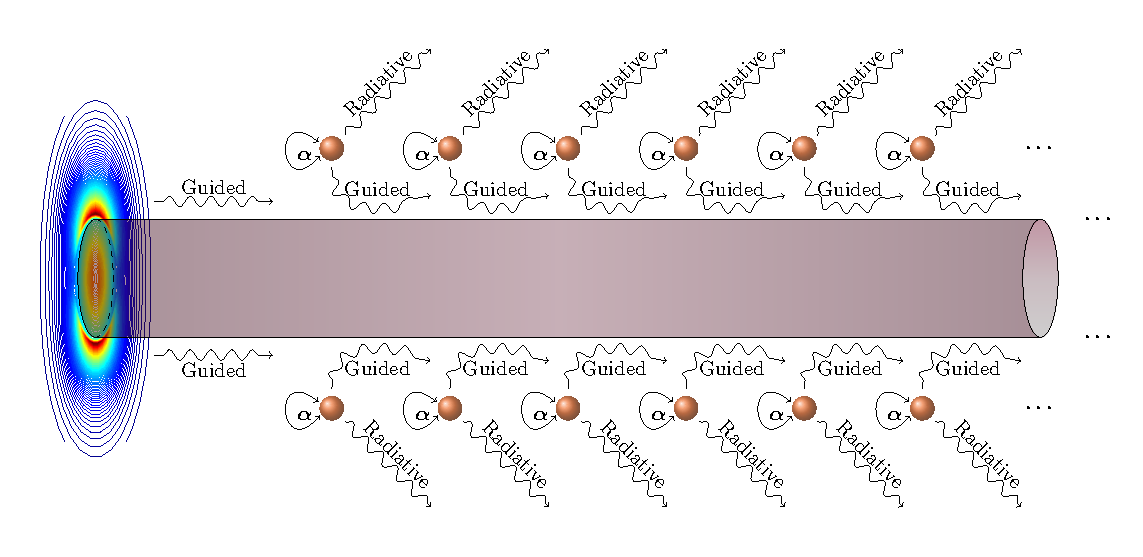
\includegraphics[width=0.85\textwidth]{../media/Figs/NanofiberTrappedAtoms}}
\caption[Guided and radiative photon emissions from atoms trapped next to a nanophotonic waveguide.]{Guided and radiative photon emissions from atoms trapped next to a nanophotonic waveguide. In the dispersive regime and when the atoms are placed a few hundred nm away from each other, the effect of the unguided radiation from the atoms can be ignored, and the photon scatterings among atoms are also negligible. For a quantum-measurement--targeted research, we mainly care about how the atomic emissions are modified by the waveguide interface and coupled to the guided modes to be detected at the measurement apparatus. Color contour on the left-hand part is an illustration of one guided mode intensity distribution of an optical nanofiber, which leaks into the free space to interact with atoms and propagates through the fiber. }\label{fig:trappedatomradiation}
\end{figure}

In this chapter, we will first outline the basic concept of the polarization state of light and introduce the experimental setup to characterize the dispersive light shift interaction, which is called \emph{polarization spectroscopy}\index{polarization spectroscopy}.
The theme of this dissertation is based on the atom-light interactions which includes two aspects: how the light responds to the presence of the atoms, and how the atoms' properties modified by the light. For the light response aspect, we will derive a general theory in the language of Green's function to formulate the atom-light interaction mainly from the semi-classical perspective where the light is treated as a continuous wave while the atom has discrete level structures. 
Figure~\ref{fig:trappedatomradiation} shows a nanofiber interface.

For the atoms' response, we will extend the definition of the polarizability of atoms from a classical oscillator picture to the multiple-level quantum representation, and then introduce the Purcell effect~\cite{Purcell1946} and derive the modified spontaneous decay rates of atoms in the presence of a waveguide using the Green's function language. 
We will show that the modifications of spontaneous emissions when atoms are placed at certain distance can be ignored.
At the end of this chapter, we will conclude with some geometric explanations on the unique features and advantages of using a nanophotonic waveguide interface to implement atom-light coupling over the free-space interface commonly employed in previous experiments.

\section{Polarization spectroscopy and dispersive light shift measures}

\subsection{Measuring the polarization state of light in free space}

The electric field of a free-propagating monochromatic light can be expressed in the Cartesian coordinate system by~\cite{Jackson1975}
\begin{align}
\mathbf{E}(\br,t) = \mathbf{E}_x(\br,t) + \mathbf{E}_y (\br,t),
\end{align}
where the $ x $ and $ y $ components
\begin{subequations}
\begin{align}
\mathbf{E}_x(\br,t) &= \mathcal{E}_{x}\mathbf{e}_x e^{i(k_0z-\omega_0 t)},\\
\mathbf{E}_y(\br,t) &= \mathcal{E}_{y}\mathbf{e}_y e^{i(k_0z-\omega_0 t)},
\end{align}
\end{subequations}
with complex amplitudes $ \mathcal{E}_{0x} $ and $ \mathcal{E}_{0y} $ in the linear polarization basis supported by the direction vectors $ \mathbf{e}_x $ and $ \mathbf{e}_y $.
We define the propagation direction of the light is along the $ z $ axis. 
Depending on the relative amplitude and phase between the $ x $ and $ y $ components, the polarization state of the light can be \emph{linear}\index{polarization!linear polarization}, \emph{circular}\index{polarization!circular polarization} and elliptical\index{polarization!elliptical polarization}~\cite{Jackson1975}.
For the convenience of describing the polarization state of light, we define the following polarization bases. 

First, we define the circular polarization basis by the complex orthogonal unit vectors
\begin{align}\label{eq:epm}
\mathbf{e}_{\pm}=\frac{1}{\sqrt{2}}(\mathbf{e}_x \pm i\mathbf{e}_y)
\end{align}
with properties
\begin{align}
\mathbf{e}_q\cdot \mathbf{e}_{q'}^* &=\delta_{q,q'}\\
\mathbf{e}_q^* &=\mathbf{e}_{-q}
\end{align}
where the field has been decomposed into the $ q=\pm $ components by 
\begin{align} 
\mathbf{E}&=\sum_q \mathcal{E}_q\mathbf{e}_q=\mathcal{E}_+ \mathbf{e}_+ +\mathcal{E}_-\mathbf{e}_-
\end{align} 
with $ \mathcal{E}_q=\mathbf{e}_q^*\cdot \mathbf{E} $.
The circular polarization components can be given by 
\begin{align}
E_\pm(\br_0,t) &= \re\left[\mathbf{e}_\pm^* \cdot \mathbf{E}\right] = \re\left[\mathcal{E}_\pm \right].
\end{align}
The $ + $ and $- $ subscripts correspond to the positive and negative helicity of circular polarizations.

Second, we define another linear polarization basis, namely, the diagonal polarization basis $ (\mathbf{e}_D,\mathbf{e}_{\thickbar{D}}) $ by 
\begin{subequations}\label{eq:eDeDbar}
\begin{align}
\mathbf{e}_D &= \frac{1}{\sqrt{2}} (\mathbf{e}_x+ \mathbf{e}_y),\\
\mathbf{e}_{\thickbar{D}} &= \frac{1}{\sqrt{2}} (\mathbf{e}_y - \mathbf{e}_x).
\end{align}
\end{subequations}
This linear polarization basis is a $ 45^\circ $ rotation from the $ (\mathbf{e}_x,\mathbf{e}_y) $ basis in the $ xy $ plane. 
One can decompose the $ \mathbf{E} $ vector in the diagonal linear polarization basis by $\mathbf{E} = \mathcal{E}_D\mathbf{e}_D + \mathcal{E}_{\thickbar{D}}\mathbf{e}_{\thickbar{D}}=E_De^{i\delta_D}\mathbf{e}_D + E_{\thickbar{D}}e^{i\delta_{\thickbar{D}}}\mathbf{e}_{\thickbar{D}} $, where $ \delta_D $ and $ \delta_{\bar{D}} $ are the phases of the two components.

The polarization state of light can be fully described by the Stokes vector $ \mathbf{S}= (S_0, S_1,S_2,S_3) $~\cite{Born1999Principles,Jackson1975}, 
where the Stokes vector components can be defined using the real amplitudes of the electric field components in those polarization bases:
\begin{subequations}\label{eq:S_intensitydiff}
\begin{align}
S_0 &= E_H^2+E_V^2 = E_+^2+E_-^2 = E_D^2+E_{\thickbar{D}}^2,\\
S_1 &= E_H^2-E_V^2,\\
S_2 &= E_D^2-E_{\thickbar{D}}^2,\\
S_3 &= E_+^2-E_-^2. %=E_L^2-E_R^2
\end{align}
\end{subequations}
Above, we have replaced $ x\rightarrow H $ and $ y\rightarrow V $.
Given that $ E_i^2 (i=H,V,L,R,D,\thickbar{D})$ are intensity components proportional to the photon fluxes of the linear and circular polarization components, $ S_0 $ is proportional to the total flux of the light, $ S_1 $ is proportional to the photon flux difference between the $ x $- and $ y $-polarization components, $ S_2 $ is proportional to the photon flux difference of the $ D $- and $ \thickbar{D} $-polarization components, and $ S_3 $ is proportional to the photon flux difference of the two circular-polarization components of the light. 
We summarize more details of the polarization state of light and properties of Stokes vectors in Appendix~\ref{chap:polarizationstokesvectors} for your reference.

In experiments, one can use waveplates and beam splitters to decompose field components in a given polarization basis, and use a pair of photon detectors to measure the photon flux of the corresponding orthogonal polarization components.
If we know the total power or intensity of the light, by measuring the photon flux difference in different polarization bases, one can find the normalized Stokes vector components and hence the polarization state of the light. 
This defines the \emph{polarization spectroscopy technique}\index{polarization spectroscopy}~\cite{Deutsch2010a,Salvail2013}.
The Stokes vector components of the light uniquely map the polarization state to a vector on the \Poincare sphere (see Fig.~\ref{fig:Poincaresphere}).

\begin{figure}[!tpb] % Poincare sphere.
   \centering\makebox[\textwidth]{
   %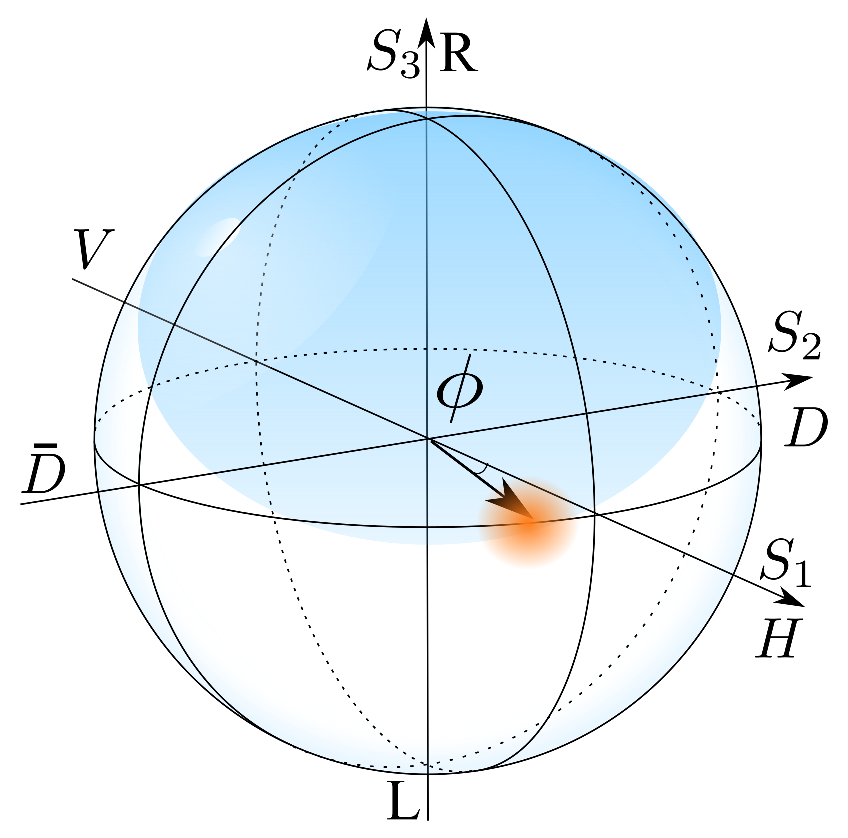
\includegraphics[width=0.55\textwidth]{../media/Figs/poincaresphere_initialS1_Faradayrot_crystal}}
   \begin{minipage}[h]{\linewidth}
    %\begin{tabular}{*{2}{b{0.2\textwidth-2\tabcolsep}}}
     \subfloat[h][]{
       %% This file was created by matlab2tikz.
%
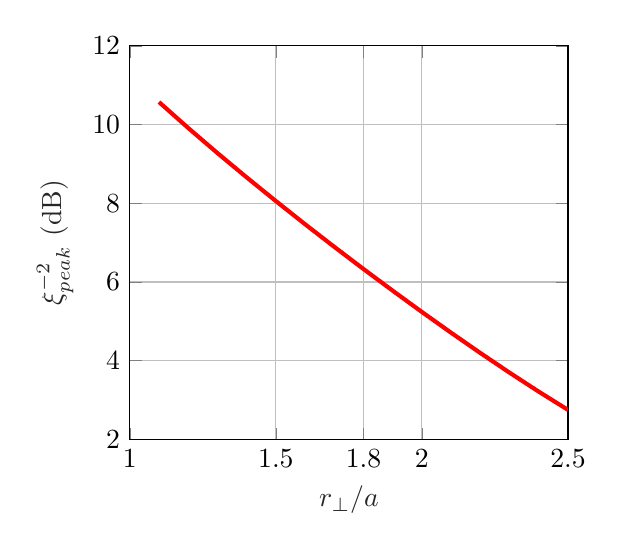
\begin{tikzpicture}

\begin{axis}[%
width=5.565cm,
height=5cm,
at={(0cm,0cm)},
scale only axis,
xmin=1.0000,
xmax=2.5000,
xtick={1.0000,1.5000,1.8000,2.0000,2.5000},
xlabel style={font=\color{white!15!black}},
xlabel={$r_\perp/a$},
ymin=2.0000,
ymax=12.0000,
ylabel style={font=\color{white!15!black}},
ylabel={$\xi^{-2}_{peak}$ (dB)},
axis background/.style={fill=white},
xmajorgrids,
ymajorgrids
]
\addplot [color=red, line width=1.5pt, forget plot]
  table[row sep=crcr]{%
1.1000	10.5712\\
1.2000	9.9128\\
1.3000	9.2762\\
1.4000	8.6588\\
1.5000	8.0571\\
1.6000	7.4685\\
1.7000	6.8935\\
1.8000	6.3307\\
1.9000	5.7799\\
2.0000	5.2394\\
2.1000	4.7118\\
2.2000	4.1974\\
2.3000	3.6980\\
2.4000	3.2157\\
2.5000	2.7531\\
};
\end{axis}
\end{tikzpicture}%
       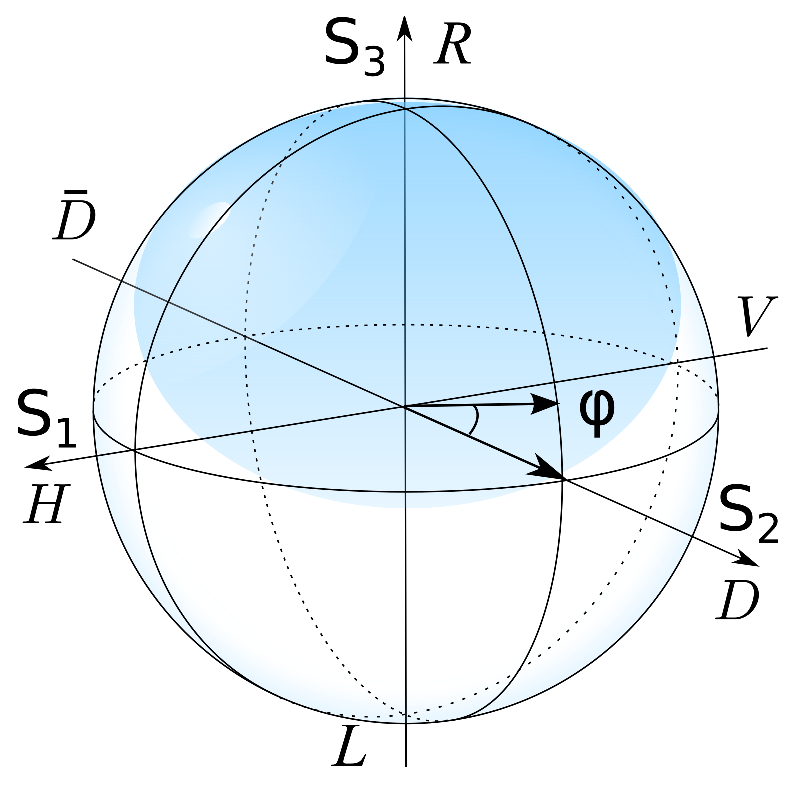
\includegraphics[width=0.4\linewidth]{../media/Figs/poincaresphere_initialS2_birefringencerot_crystal}
       \label{fig:poincaresphere_initialS2_birefringencerot_crystal}
       }
       \hfill
     \subfloat[h][]{
         \label{fig:poincaresphere_initialS2_Faradayrot_crystal}
         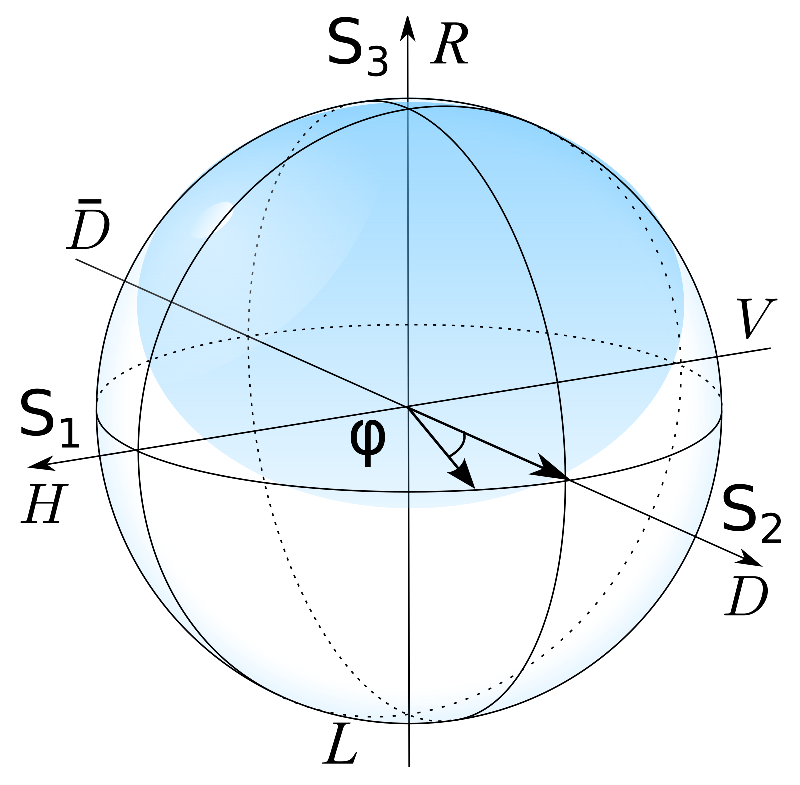
\includegraphics[width=0.4\linewidth]{../media/Figs/poincaresphere_initialS2_Faradayrot_crystal}
         %% This file was created by matlab2tikz.
%
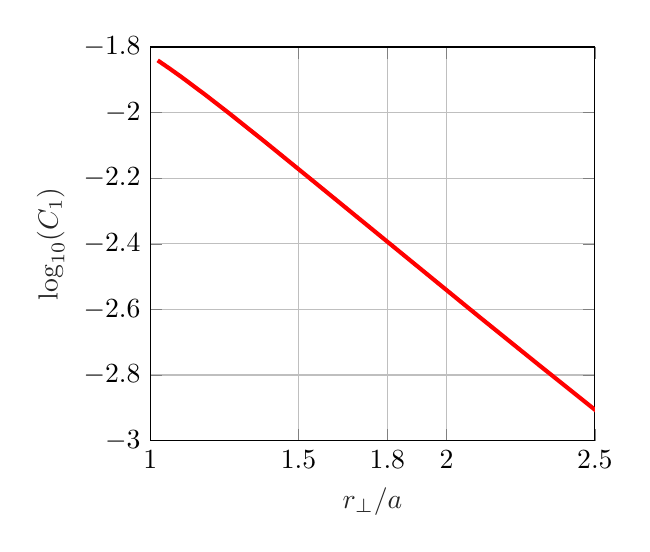
\begin{tikzpicture}

\begin{axis}[%
width=5.647cm,
height=5cm,
at={(0cm,0cm)},
scale only axis,
xmin=1.0000,
xmax=2.5000,
xtick={1.0000,1.5000,1.8000,2.0000,2.5000},
xlabel style={font=\color{white!15!black}},
xlabel={$r_\perp/a$},
ymin=-3.0000,
ymax=-1.8000,
ylabel style={font=\color{white!15!black}},
ylabel={$\log_{10}(C_1)$},
axis background/.style={fill=white},
xmajorgrids,
ymajorgrids
]
\addplot [color=red, line width=1.5pt, forget plot]
  table[row sep=crcr]{%
1.0251	-1.8409\\
1.0653	-1.8658\\
1.1055	-1.8917\\
1.1859	-1.9459\\
1.2663	-2.0022\\
1.3869	-2.0891\\
1.5477	-2.2073\\
2.1106	-2.6230\\
2.3116	-2.7696\\
2.5126	-2.9148\\
};
\end{axis}
\end{tikzpicture}%
         }
   \end{minipage}}
   \caption[Birefringence and Faraday rotations of the polarization state of light represented on the \Poincare sphere.]{Birefringence (a) and Faraday (b) rotations of the polarization state of light represented on the \Poincare sphere. A state of polarization of light can be represented as a vector $ \mathbf{S}=(S_0,S_1,S_2,S_3) $ with the Stokes parameter $ S_0 $ defining the radius of the sphere. 
   $ S_1 $, $ S_2 $ and $ S_3 $ directions correspond to a horizontal-linear ($ H $), diagonal-linear ($ D $) and circular ($ R $, with positive helicity) polarization states of light. 
   We consider a polarization state initially represented by the $ S_2 $ vector. 
   (a) If the Stokes vector rotes around $ S_1 $ or other linear-polarization axis by some angle $ \varphi $, we call this rotation as a birefringence rotation and the polarization state becomes elliptical afterwards. 
   (b) If the Stokes vector rotates about $ S_3 $ axis on the equator by some angle $ \varphi $, we call this a Faraday rotation and the helicity of the polarization state remains. 
   }
   \label{fig:Poincaresphere}
\end{figure}

For a completely polarized light\footnote{ The Stokes parameters of a partially polarized light satisfy $ S_0^2>S_1^2+S_2^2+S_3^2 $. For ``natural light" or completely unpolarized light, the Stokes parameters satisfy $ S_1=S_2=S_3=0 $. Such, the degree of polarization is defined by $ R=\frac{\sqrt{S_1^2+S_2^2+S_3^2}}{S_0} \le 1$. Throughout this dissertation work, the degree of polarization is not our concern, and we assume that the length of Stokes vectors are properly normalized.}, the Stokes parameters satisfy~\cite{Born1999Principles}
\begin{align}
S_0^2=S_1^2+S_2^2+S_3^2,
\end{align}
fixing one degree of freedom of the Stokes vectors. That leaves three independent variables to be specified to fully describe the polarization state of a light.
For example, in the linear polarization basis, the real amplitudes $ E_x $, $ E_y $ and the relative phase $ \delta_x-\delta_y $ uniquely define the polarization state of the light.
The phase difference between the two linear components of the field, $ \phi=\delta_x-\delta_y $, determines the helicity. 
The amplitudes of the two field components determine the polarization magnitude and the polarization angle from the $ x $ axis~\cite{Jackson1975}. 
Similar rules can be found for using other polarization representation bases at large~\cite{Mecozzi2011Unified}. 
On the \Poincare sphere, $ (S_1,S_2,S_3) $ can be specified by the orientation angle $ \Psi (0\le \Psi \le \pi) $ of the ellipse projected onto the $ xy $ plane, and another angle $ \Theta (-\frac{\pi}{4}\le \Theta \le \frac{\pi}{4}) $ which is the angle of the ellipse from the $ S_3 $ axis. 
That is~\cite{Born1999Principles}
\begin{align}
S_1 &= S_0\cos(2\Theta)\cos(2\Psi)\\
S_2 &= S_0\cos(2\Theta)\sin(2\Psi)\\
S_3 &= S_0\sin(2\Theta).
\end{align}
The factor of 2 reflects the symmetry of polarization. For example, a linear polarization with an oscillation vector along the positive $ x $ direction is the same as that along the negative $ x $ direction. 

When the polarization magnitude $S_0$ is fixed, we only need two free variables $ \Theta $ and $ \Psi $ to specify a state of a completely polarized light. On the \Poincare sphere, one can specify a state of polarization from a given initial state by two consecutive rotations around two orthogonal axes. 
The rotation around the $ S_1 $, $ S_2 $ or an arbitrary linear polarization axis is physically generated by the \emph{birefringence effect}\index{birefringence effect}.
The rotation around the $ S_3 $ axis is generated by the \emph{Faraday effect}\index{Faraday effect} (see Fig.~\ref{fig:polarizationspectroscopy}). 
With these two polarization transformation effects, one can generate an arbitrary polarization state of light from an initial state. 

\subsection{Polarization spectroscopy on waveguide interfaces}
Now, we turn on to atom-light interfaces with nanophotonic waveguides. 
We assume that a waveguide is designed so that the polarization of a transverse light beam in free space can be adiabatically coupled to a unique mode of the waveguide when the light travels through the waveguide. 
When the light exits the waveguide, the mode of the waveguide can again adiabatically recovers to a unique polarization state of a transverse light in free space~\cite{Nayak2007}. 
The adiabatic connection between the light's polarization states in free space and the modes in the waveguide region applies identically to the processes of incidence to and exiting from the waveguide. 
We also assume that the dispersive and distortion effects solely due to the waveguide have been compensated before the polarization state measurement or can be extracted out from the measurement result so that we can focus on the effects caused by atom-light interaction in the nanophotonic waveguide region. 
We label the waveguide mode by the polarization state of the free-space light to which the mode is adiabatically connected. 
For instance, an $ H $ mode of a nanofiber indicates the mode adiabatically connected to a linearly polarized incident light with the polarization direction along the $ x $ or $ H $ axis. To study how the atom-light interaction changes the polarization state of the light, one could simply measure the state of light in the free space, and hence the same method of polarization spectroscopy technique can be applied to the waveguide platform. A typical polarization spectroscopy experimental setup is illustrated in Fig.~\ref{fig:polarizationspectroscopy}.

\begin{figure}[ht] % Poincare sphere.
   \centering\makebox[\textwidth]{
   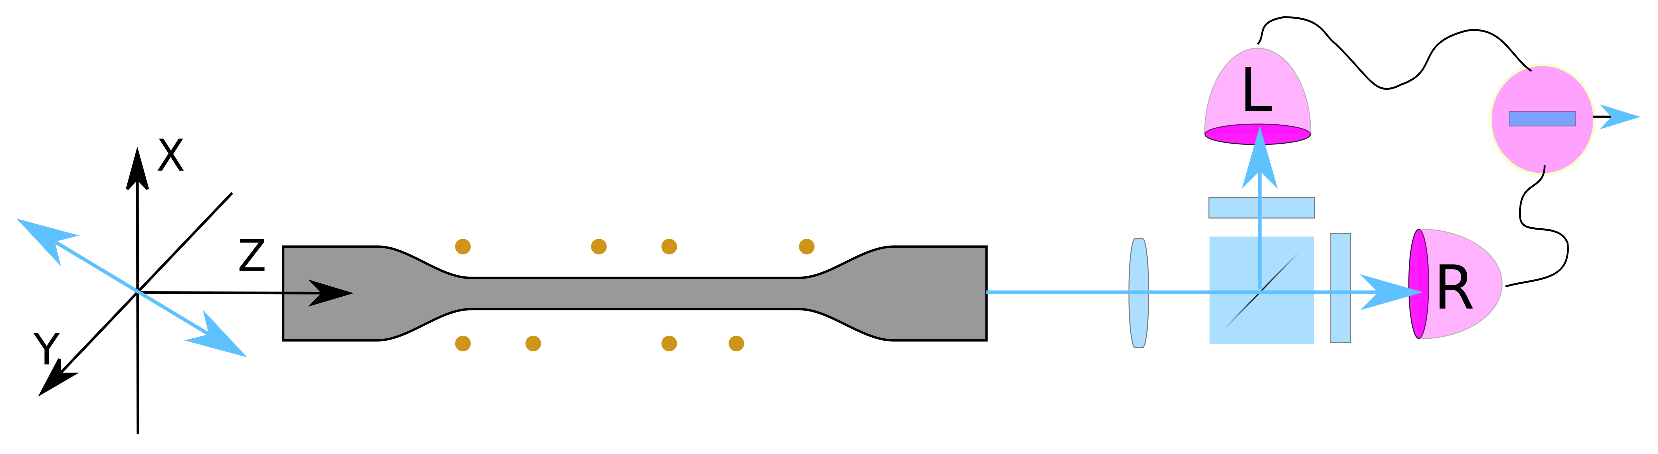
\includegraphics[width=0.85\textwidth]{../media/Figs/ProbeNanofiber_birefringence_lightpath_inputlight}}
   \caption[Polarization spectroscopy on a nanofiber platform.]{This figure shows an example of a polarization spectroscopy scheme to measure the birefringence effect (see text) due to atom-light interaction near an optical nanofiber. A light linearly polarized along the $ D $ direction (in blue) is incident to the tapered fiber and converted to the fiber's $ D $ mode that interacts with the atoms trapped near the waveguide. After the interaction with the atoms, the guided light adiabatically connect to the light in free space again. 
   Two photon detectors measuring the photon flux difference of orthogonal polarization components can be used at the end to measure the polarization state of the output. }
   \label{fig:polarizationspectroscopy}
\end{figure}

Although we will keep as general as possible, for simplicity, we will only look at single-mode waveguides that only allow degenerate fundamental modes to propagate. The rest of this dissertation will be focusing on the atom-light interaction in the nanophotonic waveguide region and the design of particular quantum measurement protocols. There are two basic light-response effects to be introduced in the following section: the \emph{birefringence effect}\index{birefringence effect} and the \emph{Faraday effect}\index{Faraday effect}.


\subsection{Birefringence and Faraday effects caused by atom-light interactions}

Consider a laser beam propagates through a cloud of atoms and generates a birefringence rotation on its polarization state. This process is possible if there is a relative speed difference of the light propagation along two orthogonal directions which are usually defined as the \emph{fast axis}\index{fast axis} and \emph{slow axis}\index{slow axis}. Correspondingly, the effective index of refraction due to the atom-light interaction along the two directions are different and denoted by $ n_f $ and $ n_s $ with $ 1\le n_f<n_s $, respectively. Therefore, there is a phase difference $ \phi $ after the light propagates by a distance $ L $, where 
\begin{align}
\phi= k(n_f-n_s)L.
\end{align}
Consequently, a linearly polarized light input may become elliptically polarized after the interaction, and the phase difference above indicates how much the Stokes vector is rotated from a linear polarization axis on the \Poincare sphere defined by the orientation of the fast axis.
Physically, how much the phase shift is generated due to the interaction with atoms determines how strong the birefringence effect is. 
Given a thickness of the atom cloud, if a linear polarization component of the light along the $ x $ axis gives the maximum phase shift after the interaction among all the other linear polarization components while the $ y $ component yields the minimum phase shift, then the $ x $ axis and the $ y $ axis define the fast axis and the slow axis, respectively. The interaction will yield a birefringence effect, rotating the Stokes vector around the $ S_1$ axis on the \Poincare sphere. 

Similar to Eq.~\eqref{eq:S_intensitydiff}, one can generalize the physical explanation of birefringence effect due to a cloud of atoms to both birefringence and Faraday effects due to atoms trapped near a waveguide by looking at the phase shift difference between two orthogonal modes.
In our study, all atoms trapped outside of a waveguide can be projected to the same position on the transverse plane of the fiber profile up to a reflection symmetry across the fiber axis. 
We see this in the tapered nanofiber experiments with atoms trapped on an optical lattice~\cite{Dawkins2011,Vetsch2010Optical}. 
If both the $ H $ mode and the $ V $ mode have the same phase shift at the atoms' position while the $ R $ mode and the $ L $ mode have different phase shifts, then the atom-light interaction will yield a Faraday rotation around the $ S_3 $ axis on the \Poincare sphere.

%In general, as a result of the atom-light interaction, the polarization of the light will experience one of the two optical effects, the birefringence effect and the Faraday effect, or a mixture of the two effects. If we denote the polarization state of the light by $ \ket{\phi} $ and quantize the Stokes vector, promoting it to a column vector operator $ \hat{\mathbf{S}}=(\hat{S}_0;\hat{S}_1;\hat{S}_2;\hat{S}_3) $, the rotation of the polarization of the light on the \Poincare sphere due to the interaction with atoms can be denoted as
%\begin{align}
%e^{i\boldsymbol{\chi}\cdot\hat{\mathbf{S}} }\ket{\phi},
%\end{align}
%where the coordinates $ \boldsymbol{\chi}=(\chi_0,\chi_1,\chi_2,\chi_3) $ are the rotation angles around $ S_i (i=1,2,3) $ axes and the photon number attenuation \nd{on?} $ S_0 $. The strength and details of the atom-light interactions hide in the $ \boldsymbol{\chi} $ vector. The key to designing particular polarization-based interactions lies on the phase response of particular waveguide modes. With this brief introduction of the polarization rotations and waveguide setups, we will dive into the beauty of atom-light interactions and inspire non-classical applications in the rest of the dissertation.

In the next section, we will look into the properties of the bare waveguide modes and the dispersive response of the waveguide modes due to the presence of the atoms from the perspective of Green's function. 

\section{Dispersive light response in the perspective of Green's function}
\subsection{Eigenmodes of a dielectric waveguide}\label{sec:eigenmodesofwaveguides}
We assume a waveguide infinitely long with uniform profile of refractive index through the fiber axis. For a nanophotonic waveguide that can trap atoms using its evanescent field, its dimension of the cross-section is smaller than the wavelength $ \lambda $ of the probe (typically, around $ \lambda=894 $ nm or $852  $ nm, which are the D1 and D2 lines of cesium atoms). 
We assume the waveguide is a linear medium with no absorption to the guided modes. The refractive bulk index\index{refractive index} of the waveguide can be given by
\begin{align}
n_0(\br_\perp) = \begin{cases} 
n_1(\br_\perp), &\quad \text{core region},\\
n_2(\br_\perp), &\quad \text{clad},
\end{cases} 
\end{align}
where $ n_1>n_2 $, $ \br_\perp=(x,y) $ are the coordinates in the transverse plane of the waveguide, and the index of refraction defined above applies to all transverse slices along the $ z $ axis which is the waveguide axis along the light propagation direction.

A monochromatic electric field propagating in such a waveguide can be given by~\cite{Jackson1975}
\begin{equation}
\mathbf{E}_0(\br,t)=\boldsymbol{\mathcal{E}}_0(\br_\perp)e^{i(b\beta z-\omega_0 t)} %+\frac{1}{2}\mathrm{c.c.}
=\mathcal{E}_0\mathbf{u}(\br_\perp)e^{i(b\beta z-\omega_0 t)}, %+\frac{1}{2}\mathrm{c.c.},
\label{Ert0}
\end{equation}
where $ b=\pm $ indicates the propagating direction, and $\boldsymbol{\mathcal{E}}_0(\br_\perp)=\mathcal{E}_0\mathbf{u}(\br_\perp)$ is the positive-frequency electric field envelope,
with $\mathcal{E}_0$ determining the field amplitude and $\mathbf{u}(\br_\perp)$ as the polarization vector at $ \br_\perp=(x,y)=(r_\perp,\phi) $ in either Cartesian or cylindrical coordinate system.
In general, $\mathcal{E}$ is a complex scalar constant and $\mathbf{u}(\br_\perp)$ is a complex vector normalized to the energy flux or the power across a transverse plane. The spatial dependent part of the field $ \mathbf{u}(\br_\perp)e^{ib\beta z} $ can be written as a linear combination of the \emph{eigenmodes}\index{eigenmode} supported by the waveguide.

The eigenmodes of a waveguide include both guided (bound) and radiation (unbound or unguided) modes, based on the corresponding waveguide boundary condition problem governed by the Maxwell equations~\cite{Jackson1975}. 

We use subscript $ \mu={j,\beta,p} $ to indicate generic guided eigenmodes, $ \mathbf{u}_\mu (\br) $, in which $ j=1 $ and $ \beta=\beta_0 $ for single-mode waveguides. 
We use mode index $ \nu=(\omega,\beta,m,p) $ to indicate unguided eigenmodes, $ \mathbf{u}_\nu(r\!_\perp ) $, where $ m=0,\,\pm 1,\,\pm 2,\cdots $ is the mode index, and $p=\pm$ denotes the polarization pattern.
One can show that (see Appendix~\ref{chap:guidedunguidedmodes}), for a guided mode, $ n_2k_0< \beta<n_1 k_0 $; for an unguided mode, $ 0<\beta <n_2 k_0 $. 

These eigenmodes satisfy the orthogonality condition,
\begin{subequations}\label{eq:eigenmodeorthog}
\begin{align}
\int d^2 \mbf{r}_\perp \, n^2(r_\perp)\mathbf{u}^*_\mu (\br_\perp) \cdot \mathbf{u}_{\mu'} (\br_\perp)\big|_{\beta = \beta'} &= \delta_{j,j'}\delta_{p,p'},\\
\int\mathrm{d}^2\br_\perp n^2(\br_\perp)\left[\mathbf{u}_{\nu}(\br\!_\perp )\cdot\mathbf{u}_{\nu'}^*(\br\!_\perp )\right]_{\beta=\beta',m=m'} &=\delta(\omega-\omega')\delta_{pp'},
\end{align}
\end{subequations}
and have dimension $1/\sqrt{A}$, where $ A $ is the area for the corresponding mode with $ \beta=\beta' $~\cite{LeKien2014}.
The completeness relations of these eigenmodes can be given by
\begin{align}
\sum_{b,p}\int \mathrm{d}\mathbf{k} \,n^2(\br_\perp)\mathbf{u}_{\mu}(r\!_\perp )\mathbf{u}_{\mu}^*(r'\!_\perp ) &= \unittensor\delta^T(r\!_\perp-r'\!_\perp),\\
\sum_{m,p}\int \mathrm{d}\mathbf{k} \, n^2(\br_\perp)\mathbf{u}_{\nu}(r\!_\perp )\mathbf{u}_{\nu}^*(r'\!_\perp ) &=\unittensor\delta^T(r\!_\perp-r'\!_\perp),
\end{align}
where $ \unittensor $ is the unit tensor, $ b=\pm $ denotes the propagation direction, and $\delta^T(r\!_\perp-r'\!_\perp)$ is the delta function for transverse fields.

%The orthogonality conditions of the guided and radiation modes can be summarized as follows: 
%\begin{align}
%\int\mathrm{d}^2\br_\perp n^2(\br_\perp)\mathbf{u}_{\mu}(\br\!_\perp )\cdot\mathbf{u}_{\mu'}^*(\br\!_\perp ) &=\delta_{\mu\mu'},\label{eq:normalu}
%\end{align}

\subsubsection{Solving the eigenmodes for a nanofiber and \SWG}
As an example, a typical optical nanofiber has a cylindrical cross-section of radius $ a $. We use $ a=225 $nm, $ n_1=1.4496 $ as a constant in the core region ($ r_\perp\le a $) and $ n_2=1.0000 $ in the vacuum clad region ($ r_\perp>a $), where we have set the $ z $ axis to be the symmetric center of the nanofiber and $ r_\perp =\sqrt{x^2+y^2} $.
Another nanophotonic waveguide is a waveguide with a square cross section, which we call a square waveguide. The waveguide has a width of $ w=300 $nm, $ n_1=2.0 $ for an ideal Si$_3$N$_4$ core medium $ (|x|\le w/2,|y|\le w/2) $, and the clad is also the vacuum\footnote{Details about our choice of the \SWG are in Appendix~\ref{chap:choozingSWGs}.}.
In both cases, only the fundamental guided modes are allowed to propagate through the waveguide. That is, the allowed guided modes have a single propagation constant\index{propagation constant} or projected wavenumber $ \beta_0 \,(n_1k_0<\beta_0<n_2k_0)$ with wavenumber\index{wavenumber} $k_0=2\pi/\lambda=\omega_0/c $, where $\omega_0$ is the angular frequency of the electric field, and $ c $ is the speed of light in a vacuum.

The fundamental modes of the nanofiber are the \HE-modes with degeneracy in propagation directions $ b=\pm $ and polarizations of two labeled by $ p $. 
For a single-mode \SWG, the quasi-\TE and the quasi-\TM modes together with a similar degeneracy in propagation directions and polarizations of two.

To calculate the eigenmodes of a dielectric waveguide, one may find analytical solutions if the waveguide has a solvable symmetry--like the cylindrical nanofiber, or one has to rely on numerical tools in most general cases--like the \SWG. 
 


The solution of the electric field and the fundamental eigenmodes of a cylindrical fiber have been solved in previous works~\cite{Snyder1983Optical,LeKien2014}. We provide a brief review of the method to solve the fiber problem in Appendix~\ref{chap:fibereigenmodes} with solutions of the \HE eigenmodes and its group velocity. The radiation mode solution is less used in this dissertation and can be found in, for example, Ref.~\cite{LeKien2014}. 

A relatively simple form for the guided eigenmodes of a nanofiber can be expressed in a cylindrical basis $(r_\perp, \phi, z)$ with longitudinal unit vector $\mathbf{e}_z$, oriented along the waveguide axis.  
The transverse unit vectors are related to their fixed Cartesian counterparts via the relations
\begin{subequations}
	\begin{align}
		\mathbf{e}_{r_{\!\perp}}     &= \mathbf{e}_x \cos \phi + \mathbf{e}_y \sin \phi, \\
		\mathbf{e}_\phi &= - \mathbf{e}_x \sin \phi + \mathbf{e}_y \cos \phi.
	\end{align}
\end{subequations}
The transverse profile for the quasicircular guided modes, $p = \pm$, is
	\begin{align} \label{Eq::QuasicircularModes_nanofiber}
		\mbf{u}_{b,\pm}(\mathbf{r}_\perp) = \big[\mathbf{e}_{r_{\!\perp}} u_{r_{\!\perp}}(r_\perp) \pm i \mathbf{e}_\phi u_\phi(r_\perp) +  i b \mathbf{e}_z  u_z(r_\perp) \big]e^{ \pm i \phi}, 
	\end{align}
and for the quasilinear guided modes, $p = \{H,V\}$, is
	\begin{subequations} \label{Eq::QuasilinearModes_nanofiber}
	\begin{align}
		\mbf{u}_{b,H}(\mathbf{r}_\perp) = & \sqrt{2} \big[ \mathbf{e}_{r_{\!\perp}} u_{r_{\!\perp}}(r_\perp) \cos \phi - \mathbf{e}_\phi u_\phi(r_\perp) \sin \phi +  ib \mathbf{e}_z  u_z(r_\perp) \cos \phi \big] \\
		\mbf{u}_{b,V}(\mathbf{r}_\perp) = & \sqrt{2} \big[ \mathbf{e}_{r_{\!\perp}} u_{r_{\!\perp}}(r_\perp) \sin \phi + \mathbf{e}_\phi u_\phi(r_\perp) \cos \phi +  ib \mathbf{e}_z  u_z(r_\perp) \sin \phi \big]. 
	\end{align}
	\end{subequations}
These modes are expressed in terms of real-valued functions $ \left[u_{r_{\!\perp}}(r_\perp), u_\phi(r_\perp), u_z(r_\perp)\right] $ of the HE$_{11}  $ modes of a nanofiber, which depend only on the radial coordinate $r_\perp$ given by Eq.~\eqref{Eq::ProfileFunctions}.

%\qxd{Need mode plots for the nanofiber and the \SWG. Codes: \url{rectwg_TETMlow_fullvector.m} and \url{fibermodestudy.m}.}
\begin{figure}[!tbp]
\centering\makebox[\textwidth]{
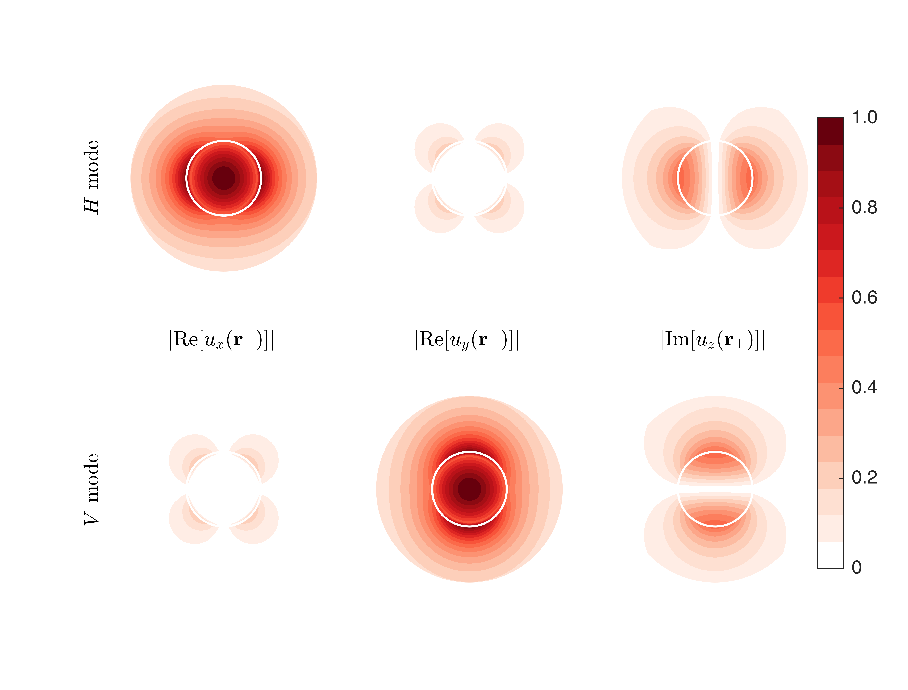
\includegraphics[width=12cm]{../media/Figs/nanofiber_HVmode_absE_xy}}
\caption[Non-zero $ H $- and $ V $-mode components of a nanofiber in the $xy $ plane.]{Non-zero $ H $ and $ V $ mode components of a nanofiber in the $xy $ plane. The first (second) row plots the $ H $($ V $)-mode components $ \left|\re\left[u_x(\br) \right]\right| $, $\left| \re\left[u_y(\br) \right]\right| $, and $\left| \im\left[u_z(\br) \right]\right| $ from left to right. Amplitudes are normalized to the maximum value of all component parts. The white lines outline the profile of the nanofiber on each subplot. }\label{fig:nanofiber_HVmode_E_xy}
\end{figure}

We plot the non-zero mode component parts of the quasilinear $ H$ and $ V $ modes of a nanofiber in Fig.~\ref{fig:nanofiber_HVmode_E_xy}.
These eigenmodes usually have non-zero longitudinal component. 
Moreover, if we place an atom on the $ x $ axis ($ \phi'=0 $), the forward-propagating $ H $ and $ V $ modes at the atom position have the following form:
\begin{subequations}\label{eq:uHVrx}
\begin{align}
\mbf{u}_{H}(\mathbf{r}'_\perp) = & \sqrt{2} \big[ \mathbf{e}_{r_{\!\perp}} u_{r_{\!\perp}}(r_\perp') +  i \mathbf{e}_z  u_z(r_\perp') \big] \\
\mbf{u}_{V}(\mathbf{r}'_\perp) = & \sqrt{2}  \mathbf{e}_\phi u_\phi(r_\perp') , 
\end{align}
\end{subequations}
where the $ H $ mode is elliptically polarized, and the $ V $ mode is linearly polarized. 
Putting the atom on the $ y $ axis gives a similar result by exchanging the $ H $ and $ V $ labels from Eq.~\eqref{eq:uHVrx}. 

\begin{figure}[!tbp]
\centering\makebox[\textwidth]{
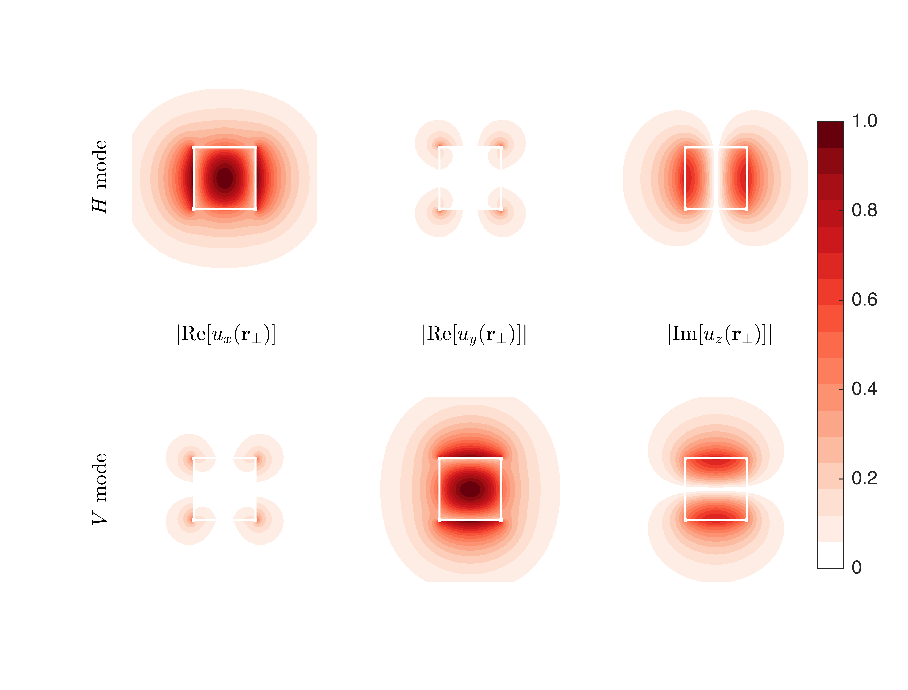
\includegraphics[width=12cm]{../media/Figs/swg_HVmode_absE_xy}}
\caption[Non-zero $ H $- and $ V $-mode components of a square waveguide in the $xy $ plane.]{Non-zero $ H $ and $ V $ mode components of a \SWG in the $xy $ plane. The first (second) row plots the $ H $($ V $)-mode components $\left| \re\left[u_x(\br) \right]\right| $, $\left| \re\left[u_y(\br) \right]\right| $, and $ \left|\im\left[u_z(\br) \right]\right| $ from left to right. Amplitudes are normalized to the maximum value of all component parts. The white lines outline the profile of the square waveguide on each subplot. }\label{fig:swg_HVmode_E_xy}
\end{figure}
ref
For the \SWG and general geometries, we solve the eigenmodes using a numerical method called \emph{Boundary Element Method}\index{Boundary Element Method} or BEM~\cite{Fallahkhair2008}. This method divides the regions close to the waveguide boundaries into finite grids and solve the wave equations by matching the boundary conditions on the grids. 
The wave equations are discretized to a set of linear equations. The eigenmodes are found by solving the eigenvalue problem defined by the boundary condition in the frequency domain. 
It is fairly efficient when we have a fixed frequency point. 
We verify the accuracy of the BEM calculation with the nanofiber case since we know the analytical solution. Then we use BEM to solve the eigenmodes for the \SWG geometry. 
By find the propagation constant $ \beta $ of the guided eigenmode as varying $ \omega $, we can solve for the group velocity $ v_g=\left.\dd{\omega}{\beta}\right|_{\beta=\beta_0} $ and the group index of refraction\index{group index of refraction} $n_g = \frac{c}{v_g}=\left.\dd{\beta}{k}\right|_{\beta=\beta_0}$.



The quasi-\TE and quasi-\TM modes are eigenmodes of the \SWG with orthogonal polarizations and can be adiabatically connected to the $ x $- and $ y $-polarized linear free-space light inputs. Therefore, we can define the quasi-\TE and quasi-\TM modes as the $ H $ and $ V $ modes for the \SWG geometry.
We plot the non-zero mode component parts of the quasilinearly $ H $ and $ V $ modes of a \SWG in Fig.~\ref{fig:swg_HVmode_E_xy}.
As shown, the field on the $ y $ axis of the $ H $ mode is also purely linearly polarized along the $ x $ direction. The electric fields on the $ x $ axis of the $ H $ mode are also elliptically polarized with the $ x $ component and the out-of-phase $ z $ component.



%As an aside, here are the reasons why we only consider a \SWG with a width of $ 300 $ nm besides the long-studied nanofiber case. In fact, on the course of this study, we have considered ridge and other types of waveguides. Eventually, we decided to study a simple shape of waveguides--a \SWG--as a proof of principles. There has also been a long discussion on purposefully designing a rectangular waveguide and imperfections on fabricating a \SWG, in which a \SWG essentially becomes a rectangular one. \nd{Do you mean that the discussion leads to the choice of a square waveguide?} Based on some back-of-envelope calculations and simple simulations, we find that, to be useful, a rectangular waveguide might have to be very long to fabricate and, if we choose a width of $ 300$--$320 $ nm, the imperfections in fabricating a \SWG processes would not generate noticeable influence on the physical effects we care about. As these reasonings involve the knowledge we are going to introduce later, 

\subsubsection{Mode superposition and decomposition}
\begin{figure}[!tbp]
\centering\makebox[\textwidth]{
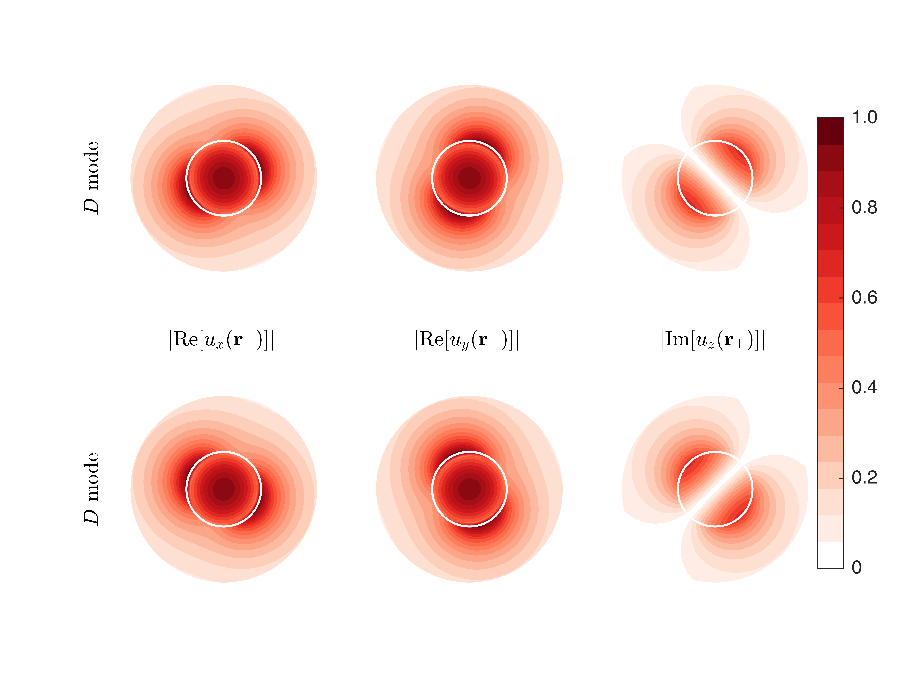
\includegraphics[width=12cm]{../media/Figs/nanofiber_DaDmode_absE_xy}}
\caption[Non-zero $ D $- and $ \bar{D} $-mode components of a nanofiber in the $xy $ plane.]{Non-zero $ D $ and $ \thickbar{D} $ mode components of a nanofiber in the $xy $ plane. The first (second) row plots the $ D $($ \thickbar{D} $)-mode components $\left| \re\left[u_x(\br) \right]\right| $, $ \left|\re\left[u_y(\br) \right]\right| $, and $\left| \im\left[u_z(\br) \right]\right| $ from left to right. Amplitudes are normalized to the maximum value of all component parts. }\label{fig:nanofiber_DaDmode_E_xy}
\end{figure}

%\begin{figure}[!tbp]
%\centering\makebox[\textwidth]{
%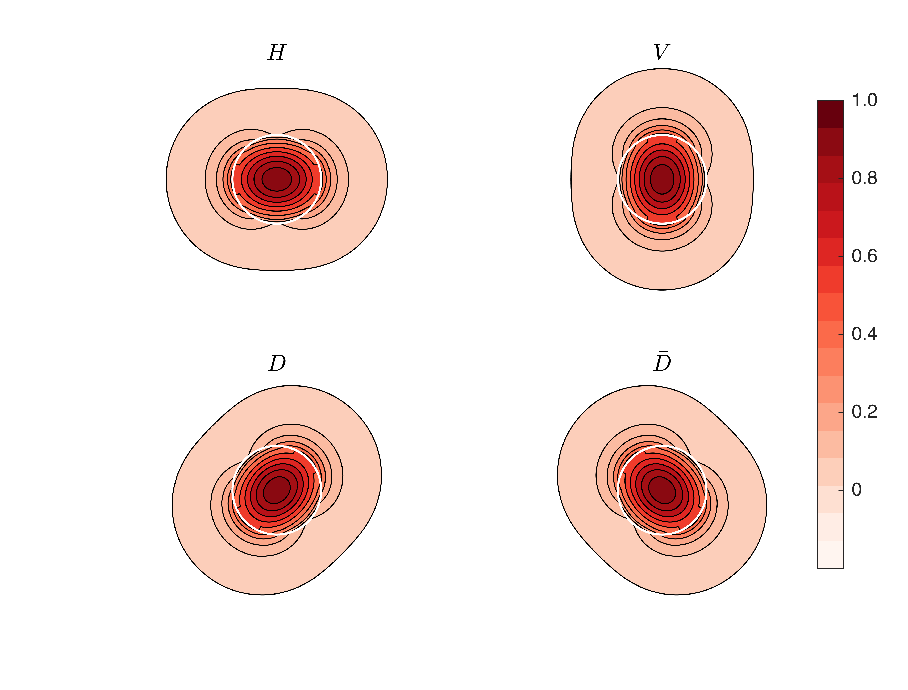
\includegraphics[width=12cm]{../media/Figs/nanofiber_HVDaDmode_Ints_xy}}
%\caption[Intensity distributions of quasi-linearly polarized modes  in the $xy $ plane of a nanofiber.]{Intensity distributions of quasi-linearly polarized modes  in the $xy $ plane of a nanofiber. }\label{fig:nanofiber_HVDaDmode_Ints_xy}
%\end{figure}

The degeneracy in polarizations of the \HE modes allows one to write the eigenmodes of the nanofiber in an arbitrary polarization basis. 
Two convenient guided-mode bases are the quasilinear and quasicircular polarization modes. 
%In Figs.~\ref{fig:Modes_Rot45HV_fiber} and~\ref{fig:Modes_Rot45LR_fiber}, we show the decomposition of a diagonally polarized $ D $ mode of a nanofiber in the $ HV $- and $ LR $-bases, respectively. 
Based on Eq.~\eqref{eq:eDeDbar}, the $ D $ and $ \bar{D} $ mode bases can be written as a linear combination of the $ H $ and $ V $ modes [see Fig.~\ref{fig:Modes_Rot45HV_fiber}]. We plot the non-zero component parts of the $ D $ and $ \bar{D} $ modes in Fig.~\ref{fig:nanofiber_DaDmode_E_xy}.
%We also plot the intensity distribution of $ H $, $ V $, $ D $ and $ \bar{D} $ modes of a nanofiber in Fig.~\ref{fig:nanofiber_HVDaDmode_Ints_xy} for comparison. 
The quasicircular polarization mode bases can be found from the $ H $ and $ V $ modes. 
In other words, a quasilinear mode can be decomposed into the quasicircular mode bases, Fig.~\ref{fig:Modes_Rot45LR_fiber}.
We find that the $ H $ mode component has a much stronger intensity at the atom position than the $ V $ mode component as shown in Fig.~\ref{fig:Modes_Rot45HV_fiber}, if we place an atom on the $ x $ axis.
This property of \emph{mode anisotropy}\index{anisotropy of waveguide modes} in azimuthal direction is intrinsic to the waveguides but does not exist in freely propagating fundamental Gaussian laser beams typically used in atom-light coupling experiments. In contrast, the decomposed $ R $ and $ L $ modes at the atom position have the same intensity. 
As we will see later, we can choose a good mode basis based on the atomic internal structure and fully utilize the isotropic property of waveguide modes, which is the key to optimally designing some quantum operations and yields great advantages for the nanophotonic waveguides over the free-space atom-light quantum interface. For now, we pave some necessary foundations.

\begin{figure}
\centering\makebox[\textwidth]{
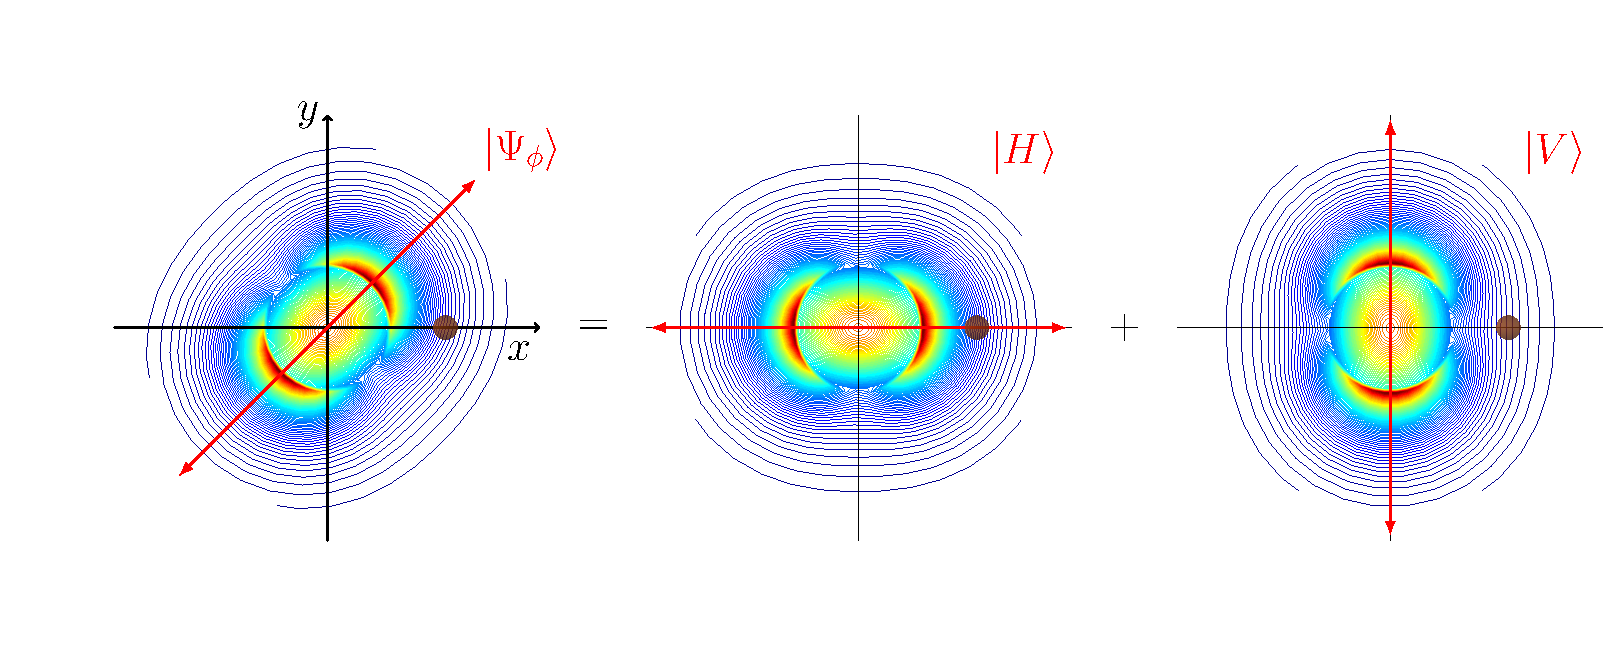
\includegraphics[width=12cm]{../media/Figs/Modes_Rot45HV}}
\caption[Mode decomposition of an input quasilinear polarized laser beam in the $ H$ and $V$ mode basis.]{Mode decomposition of an input quasilinear polarized $ D $ mode in the $ H $ and $ V $ mode basis of a nanofiber. Red double-arrowed lines indicate the linear polarization directions of the free-space mode correspondence. This figure shows that the decomposition relation $ D=(H+V)/\sqrt{2} $. 
We put a dark dot on the $ x $ axis of each mode plot to highlight the anisotropy of modes (see text). }\label{fig:Modes_Rot45HV_fiber}
\end{figure}

\begin{figure}[!tbp]
\centering\makebox[\textwidth]{
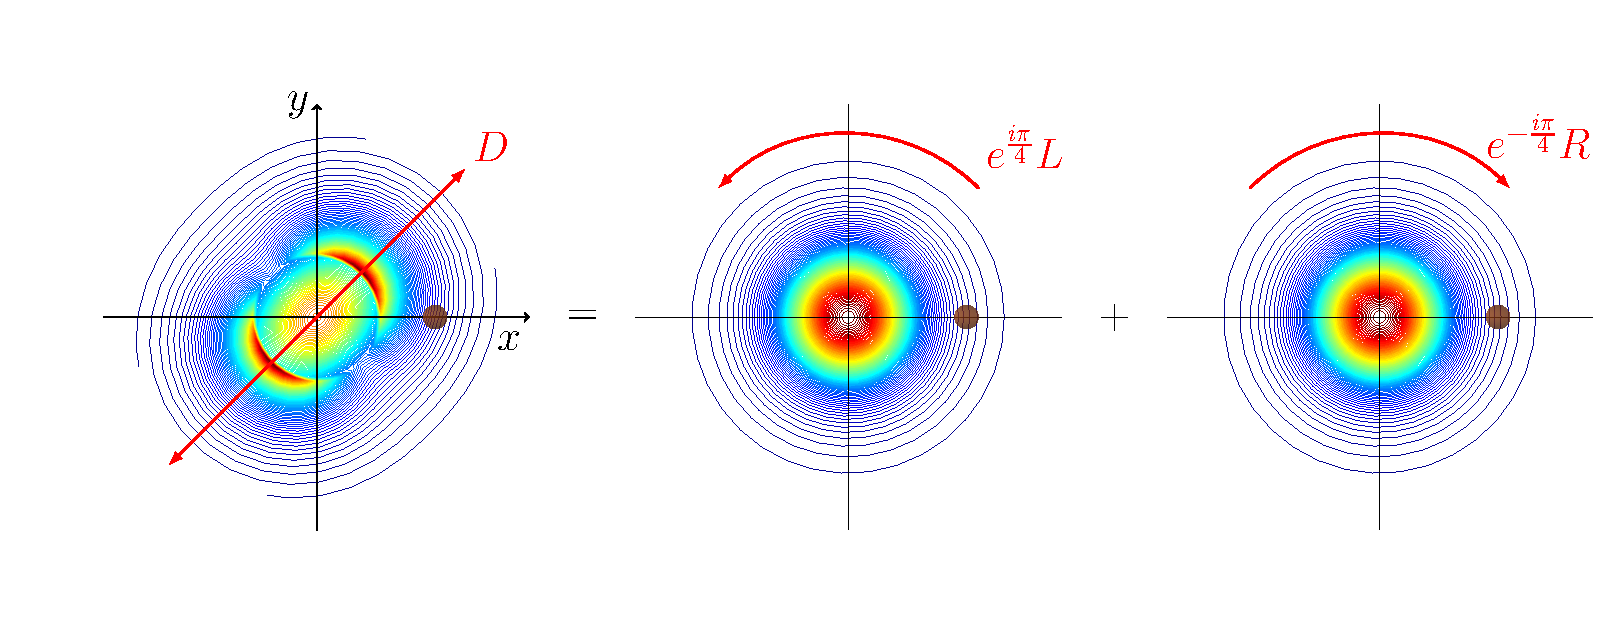
\includegraphics[width=12cm]{../media/Figs/Modes_Rot45LR}}
\caption[Mode decomposition of an input quasilinear polarized laser beam in the quasicircular mode basis.]{Same as Fig.~\ref{fig:Modes_Rot45HV_fiber} but decomposed in the $ LR$-mode basis. At the dark dot's position, the $ L $ and $ R $ modes have the same intensity.}\label{fig:Modes_Rot45LR_fiber}
\end{figure}

For the \SWG case, similarly, we can define the quasilinear $ D $ and $ \bar{D} $ modes using the $ H $ and $ V $ mode basis with non-zero components plotted in Fig.~\ref{fig:swg_DaDmode_E_xy}. 
We plot the intensity distribution of these quasilinear modes of a \SWG in the $ xy $ plane in Fig.~\ref{fig:swg_HVDaDmode_Ints_xy}. These quasilinear modes have similar anisotropic properties as the fiber modes do.



\begin{figure}[!tbp]
\centering\makebox[\textwidth]{
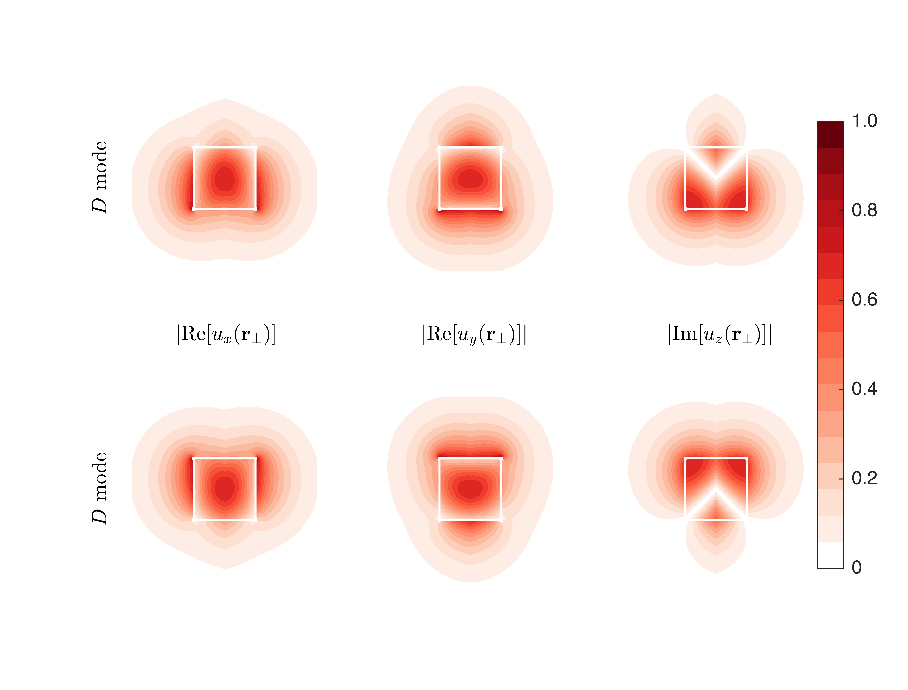
\includegraphics[width=12cm]{../media/Figs/swg_DaDmode_absE_xy}}
\caption[Non-zero $ D $- and $ \bar{D} $-mode components of a square waveguide in the $xy $ plane.]{Non-zero $ D $ and $ \thickbar{D} $ mode components of a \SWG in the $xy $ plane. The first (second) row plots the $ D $($ \thickbar{D} $)-mode components $ \left|\re\left[u_x(\br) \right]\right| $, $\left| \re\left[u_y(\br) \right]\right| $, and $\left| \im\left[u_z(\br) \right]\right| $ from left to right. Amplitudes are normalized to the maximum value of all component parts. }\label{fig:swg_DaDmode_E_xy}
\end{figure}

\begin{figure}[!tbp]
\centering\makebox[\textwidth]{
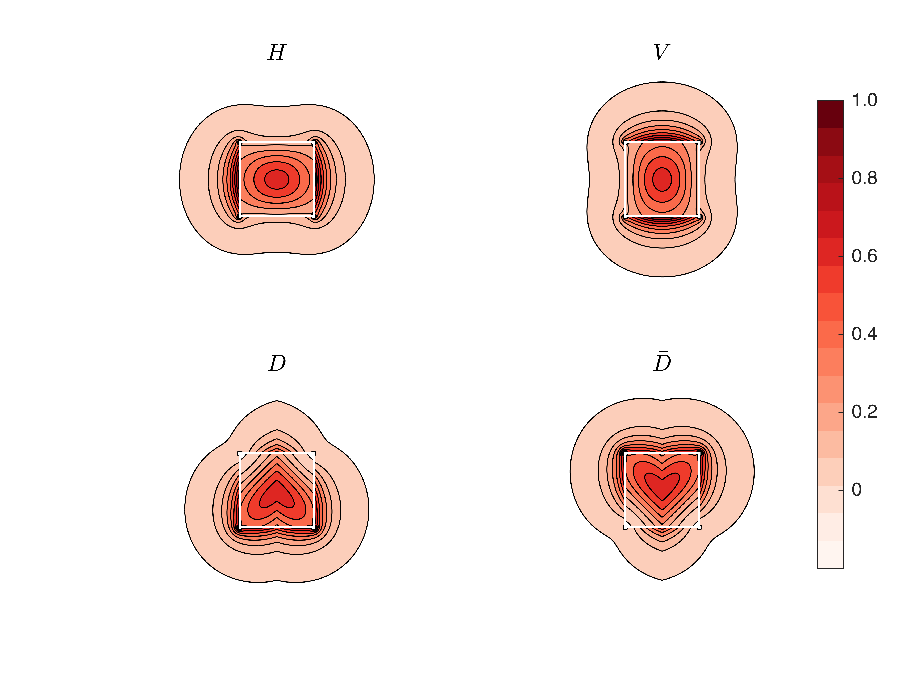
\includegraphics[width=12cm]{../media/Figs/swg_HVDaDmode_Ints_xy}}
\caption[Intensity distributions of quasilinearly polarized modes in the $xy $ plane of a square waveguide.]{Intensity distributions of quasilinearly polarized modes in the $xy $ plane of a \SWG. }\label{fig:swg_HVDaDmode_Ints_xy}
\end{figure}


\subsection{Dyadic Green's functions of dipole radiations in presence of a dielectric waveguide}\label{sec:calculatingGreenstensor}
We consider light response in the presence of a photon emitter outside of a dielectric waveguide. The dyadic Green's function\index{dyadic Green's function}, or Green's tensor\index{Green's tensor}\footnote{We may also call it Green's function tensor\index{Green's function tensor} or Green's function dyad\index{Green's function dyad}.}, $ \GFT(\br,\br')=\GFT(\br,\br';\omega_0) $ is naturally a response function of the field measured at $ \br $ responding to a unit radiating point source at $ \br' $ at a frequency $ \omega_0 $. With the dyadic Green's function, a field response due to an arbitrary source can be calculated. In this section, we consider a scenario that atoms are trapped near a nanophotonic waveguide, and formulate a general theory of field response using the Green's function method. For simplicity, we regard atoms as optical dipoles, which interact with light in terms of optical dipole radiation. The dipoles oscillate in space and time to form a current, $ \mathbf{J} $, which collectively generates an effective susceptibility for the atomic ensemble as a ``medium" and modulates the phase and amplitude of the light passing through the waveguide. 

Given the index of refraction distribution function $ n(\br) $ with the waveguide as the background medium, a chromatic electric field modulated by the presence of atoms can be described by the wave equation below~\cite{Jackson1975}: 
\begin{align}\label{eq:Maxwellwithsource2}
\left[\! -\! \nabla\!\!\times\!\nabla\!\!\times + n^2\!(\br)\frac{\omega_0^2}{c^2} \right]\!\! \boldsymbol{\mathcal{E}}(\br) &\!=\! -i4\pi\! \frac{\omega_0}{c^2}\! \mathbf{J}(\br) \!=\! -4\pi\! \frac{\omega_0^2}{c^2}\! \mathbf{P}(\br)\!=\! -4\pi\! \frac{\omega_0^2}{c^2}\! \tensor{\boldsymbol{\chi}}(\br)\! \cdot\! \boldsymbol{\mathcal{E}}(\br),
\end{align}
where the only difference from the homogeneous wave equation, Eq.~\eqref{MaxwellHelmholtz0}, is that we have brought in dipole source terms represented by the equivalent expressions on the right-hand side of the equation. For the source terms, we have defined the source of the current\index{current source} $ \mathbf{J}(\br)=\pp{\mathbf{P}}{t}=-i\omega\mathbf{P}(\br)=-i\omega_0 \tensor{\boldsymbol{\chi}}(\br)\cdot \boldsymbol{\mathcal{E}}(\br) $ with electric susceptibility\index{electric susceptibility} $ \tensor{\boldsymbol{\chi}}(\br) = \sum_{\br'}\delta(\br-\mathbf{r}')\tensor{\boldsymbol{\alpha}} \, (\br')$ \footnote{We have used the Gaussian-cgs units here. In the SI units, the corresponding relationship is $ \tensor{\boldsymbol{\chi}}(\br) = \sum_{\br'}\delta(\br-\mathbf{r}')\tensor{\boldsymbol{\alpha}} \, (\br')$ and $\tensor{\boldsymbol{\chi}}{}^{SI}=4\pi\tensor{\boldsymbol{\chi}}{}^{G}  $. Here, $ 4\pi $ is a typical multiplier factor between the SI and the Gaussian-cgs unit systems. }, where $ \tensor{\boldsymbol{\alpha}} $ is the polarizability tensor\index{polarizability!polarizability tensor} of the atoms located at $ \br' $. Specifically, using the dipole approximation, the polarizability due to the presence of atoms, $ \mathbf{P}(\br)=\sum_{\br'}\delta(\br-\br')\mathbf{d}(\br')=\sum_{\br'}\delta(\br-\br')\tensor{\boldsymbol{\alpha}} \, (\br')\cdot \boldsymbol{\mathcal{E}}(\br) $, where $ \mathbf{d}(\br') $ is the induced dipole moment of an atom at $ \br' $. 

Eq.~\eqref{eq:Maxwellwithsource2} can be solved by finding the corresponding dyadic Green's function\index{Green's function!dyadic Green's function} in the frequency domain defined by\footnote{Although the definition of the source term is arbitrary, to make the relation between $ \mathbf{E}(\br) $ and the dyadic Green's function $ \GFT(\br,\br') $ consistent with our later expressions, we have chosen the source term self-consistently. 
If we define the Green's function by $\left[ -\nabla\times\nabla\times + n^2\frac{\omega_0^2}{c^2} \right] \GFT(\br,\br') = \delta^{(3)}(\br-\br')\unittensor$ and the source term by $\tensor{\bf S}(\br)=-4\pi \frac{\omega_0^2}{c^2} \tensor{\boldsymbol{\chi}}(\br)$, which has a $4\pi\omega_0^2/c^2$ factor compared to our definition in the text, the $4\pi\omega_0^2/c^2$ factor will be carried over to the relation between $ \mathbf{E}(\br) $ and $ \GFT(\br,\br') $ and other quantities as well. Also see Ref.~\cite{Wubs2004} as another commonly used definition.}
\begin{align}
\left[ -\nabla\times\nabla\times + n^2\frac{\omega_0^2}{c^2} \right] \GFT(\br,\br';\omega_0) &= -4\pi \frac{\omega_0^2}{c^2}\delta^{(3)}(\br-\br')\unittensor. \label{eq:dyadicGF}
\end{align}

A special case of the dyadic Green's function is when a dipole source is placed in a homogeneous medium, say, the vacuum. In this case, the Green's tensor is given by
\begin{align}
\GFT(\br,\br') &=  \left[\unittensor + \frac{1}{k_0^2}\nabla\nabla \right]G_0(\br,\br')
\end{align}
with a scalar Green's function 
\begin{align}
G_0(\br,\br';\omega_0) =k_0^2\frac{e^{\pm i\mathbf{k}_0\cdot (\mathbf{r}-\br')}}{|\br-\br'|},\label{eq:G0rrp}
\end{align}
where we only need to keep the positive frequency solution for outgoing radiations. This result reflects the fact that the field responded at $ \br $ is a free spherical wave coming out from a point dipole source as we can recognize from basic electromagnetism. This solution is a key to solve radiation problems and normalize modified decay rates of atoms in the presence of a waveguide as we will discuss later. When $ \br\rightarrow \br' $ or the field responded at the dipole position, the real part of the Green's function diverges yet the imaginary part of $ G_0(\br,\br') $ takes the form
\begin{align}\label{eq:G0}
G_0=\im\left[ G_0(\br',\br')\right]=\frac{2}{3}k_0^3.
\end{align}
The details of solving the free-space Green's function and techniques we are going to use, including Born approximation~\cite{Gubernatis1977Born} and other general methods of solving a radiation problem, can be found in Appendix~\ref{chap:freespacegreenfunction}. 

The output field as Lippmann-Schwinger equation\index{Lippmann-Schwinger equation} (the first line in the equation below) after interacting with $ N_A $ atoms placed at $ \br'=\br'_n (n=1,2,\cdots,N_A) $
\begin{subequations}
\begin{align}\label{eq:Lippmann-Schwinger}
\mathbf{E}(\br) &=\mathbf{E}_0(\br)+ \sum_n^{N_A} \GFT(\br,\br'_n)\cdot \tensor{\boldsymbol{\alpha}}{}^{(n)}\cdot \mathbf{E}(\br'_n)\\
&\approx \mathbf{E}_0(\br)+ \sum_n^{N_A} \GFT(\br,\br'_n)\cdot \tensor{\boldsymbol{\alpha}}{}^{(n)}\cdot \mathbf{E}_0(\br'_n)\label{eq:EGFTnatoms}
\end{align}
\end{subequations}
where $ \tensor{\boldsymbol{\alpha}}^{(n)} $ is the polarizability of the atom positioned at $ \br'_n $. 
The right hand side of Eq.~\eqref{eq:EGFTnatoms} implies that the total field after the interaction includes two sources of fields: one is the original propagating field through the waveguide (the first term), and the other is the scattered field due to the presence of the atoms (the second term). 
Using the Born approximation, the photon scattering among atoms and high-order scattering generating self-polarizations have been ignored. 
This approximation is valid in the dispersive regime, which can be verified based on Ref.~\cite{Asenjo-Garcia2017Atom} including the atom-atom interactions and other scattering effects~\footnote{See, for example, Eq.~(10) in Ref.~\cite{Asenjo-Garcia2017Atom}. It describes the field transformation relations and will recover to our result presented in Eq.~\eqref{eq:EGFTnatoms} if the detuning $ \Delta_A $ is much larger than the frequency shift $ J_{\xi,\mathrm{1D}} $ and the modified decay rates $ \Gamma_{\xi,\mathrm{1D} }$ of atoms for dispersive interactions.}. Now, the only barrier for fully solving the output electric field is to solve the dyadic Green's function.

In general, there are two strategies to solve the dyadic Green's function: one is to solve the dipole radiation problem numerically and/or analytically; the other involves eigenmode decomposition and only needs bare waveguide modes. We call the first approach the \emph{normalization} approach, and the other the \emph{eigenmode-decomposition} approach. We will describe the two approaches in the successive subsections. 

\subsubsection{a. The \emph{normalization} approach}

We recall the equation governing the dyadic Green's function,
\begin{align}
\left[ -\nabla\times\nabla\times + n^2\frac{\omega^2_0}{c^2} \right] \GFT(\br,\br') &= -4\pi k_0^2\delta^{(3)}(\br-\br')\unittensor,
\end{align}
each column of which can be expressed as
\begin{align}
\left[ -\nabla\times\nabla\times + n^2\frac{\omega^2_0}{c^2} \right] \mathbf{G}_i(\br,\br') &= -4\pi k_0^2\mathbf{e}_i\delta(\br-\br'), \label{eq:Gi}
\end{align}
where the subscripts $ i=r\!_\perp,\phi,z $ written in the cylindrical coordinate system or $ i=x,y,z $ in the Cartesian coordinate system denote the coordinate components. The $ \mathbf{G}_i(\br,\br') $ in the equation above is the $ i$th column of the dyadic Green's function of $ \GFT(\br,\br') $. Here, we have used $\omega_0$ to indicate the angular frequency of the radiation from the source.  

Comparing Eq.~\eqref{eq:Gi} with Eq.~\eqref{eq:Maxwellwithsource2}, we find that Eq.~\eqref{eq:Gi} is exactly the chromatic wave equation of $ \mathbf{E}(\br) $ when there is a unit dipole source orientated along $ \mathbf{e}_i $ and placed at $ \br' $. That is to say, once we solve the electric field components with a unit dipole source orientated along all the $ \mathbf{e}_i $ directions, the columns of the dyadic function is just the corresponding field components. Concretely, in the cylindrical coordinate system, the dyadic Green's function elements correspond to the following electric field components emitted by a unit dipole source orientated in the three orthogonal basis directions:
\begin{equation}
\GFT(\mathbf{r},\mathbf{r}')=\!\!\!\!\!\!\!\!\!\!\!\!\!\!\!\!\!\!\!\!\!\!\!\! \!\!\!\!\!\!\!\! \!\!\!\!\!\!\!\! \!\!\!\!\!\!\!\!
  \begin{tikzpicture}[baseline=-\the\dimexpr\fontdimen22\textfont2\relax ]
   \matrix (m)[matrix of math nodes,left delimiter=(,right delimiter=),ampersand replacement=\&] % Note: the ampersandreplacement line redefines to use \& instead of the usual & sign to separate columns in the matrix. This can avoid potential conflict with external environment where ampersands are also defined for specific purposes. See https://tex.stackexchange.com/questions/15093/single-ampersand-used-with-wrong-catcode-error-using-tikz-matrix-in-beamer
  {
  G_{r\!_\perp r\!_\perp} \& G_{r\!_\perp\phi} \& G_{r\!_\perp z}\\
  G_{\phi r\!_\perp} \& G_{\phi\phi} \& G_{\phi z} \\
  G_{zr\!_\perp} \& G_{z\phi} \& G_{zz} \\
  };
  % Hightlight columns.
  \begin{pgfonlayer}{myback}
    \fhighlight[red!30]{m-1-1}{m-3-1}
    \fhighlight[blue!30]{m-1-2}{m-3-2}
    \fhighlight[green!30]{m-1-3}{m-3-3}
  \end{pgfonlayer}
  % Make links to other equivalent expressions.
  \begin{pgfonlayer}{myback}
    \draw (m-3-1.south)+(-0.5,-0.76) node [left] {column vector $\mathbf{G}_i$:};
    \draw[implies-implies,double equal sign distance] (m-3-1.south)+(0,-0.08) -- +(0,-0.5) node[below]{$ \mathbf{G}_{r\!_\perp} $};
    \draw[implies-implies,double equal sign distance] (m-3-2.south)+(0,-0.08) -- +(0,-0.5) node[below]{$ \mathbf{G}_{\phi} $};
    \draw[implies-implies,double equal sign distance] (m-3-3.south)+(0,-0.1) -- +(0,-0.55) node[below]{$ \mathbf{G}_z $};
    \draw (m-3-1.south)+(-0.5,-1.7) node [left,align=center] {equivalent $ \mathbf{E} $ radiated\\ from a unit dipole:};
    \draw[<-] (m-3-1.south)+(0,-1.08) -- +(0,-1.5) node[below]{$ \mathbf{d}_{r\!_\perp} $};
    \draw[<-] (m-3-2.south)+(0,-1.08) -- +(0,-1.5) node[below]{$ \mathbf{d}_{\phi} $};
    \draw[<-] (m-3-3.south)+(0,-1.1) -- +(0,-1.55) node[below]{$ \mathbf{d}_z $};
    %\draw[<-] (m-3-3.south)+(0.5,-1.32) -- +(1.1,-1.32) node[right]{$\cdot (-4\pi k^2)$}; % The old normalization factor.
  \end{pgfonlayer}
  \end{tikzpicture}
\end{equation}
Note that all calculations are performed with a fixed frequency $ \omega_0 $. Alternatively, we calculate the $ ij $th element of the dyadic Green's function by
\begin{align}\label{eq:GFTijEd}
G_{ij}(\br,\br';\omega_0) =\frac{E^i_j(\br)}{d^{(j)}(\br')},
\end{align}
where $ d^{(j)}(\br') $ is the dipole moment of a dipole at $ \br' $ with an orientation along the $ \mathbf{e}_j $ direction, and $ E^i_j(\br) $ is the $ i $th component of the calculated electric field responded at $ \br $ in the presence of the dipole source.
Therefore, the key to calculate the dyadic Green's function in this approach is to solve the field emitted by a normalized dipole in the presence of the waveguide in the frequency domain. In fact, there are many ways to calculate the fields with a dipole source in a medium. 

\textbf{Analytical solutions:} The field can be analytically solved only if the waveguide has some special geometry. A nanofiber geometry is one example that can be solved analytically.  
In Appendix~\ref{sec:boundrad}, we provide some details of solving the $ \mathbf{E}(\br) $ field radiated from three orthogonal unit dipoles by decomposing the dipole radiation function described by Eq.~\eqref{eq:G0rrp} into the cylindrical coordinate basis. We solve the guided mode and the radiation mode contributions via finding residues of poles and contour integrals of branch cuts. In the end, complex integrations are simplified to be over the real axis to assuming the waveguide is lossless. 
Using this method, we are able to decompose the responding Green's tensor outside of the waveguide to a part due to free-dipole radiation, $ \GFT_0(\br,\br') $, and a part due to the reflection from the waveguide interface, $ \GFT_R(\br,\br') $; and we interpret the Green's tensor responding inside of the waveguide medium, $ \GFT_T(\br,\br') $, as a result of mode transmission. Each part is calculated by projecting the total dipole radiation into the corresponding orthonormal modes. Therefore, the dyadic Green's function can be written as
\begin{align}\label{eq:GFTdecomp0RT}
\GFT(\br,\br') = \left\{ 
\begin{array}{lc}
\GFT_0(\br,\br')+\GFT_R(\br,\br'), & \br\text{ outside of the waveguide}\\
\GFT_T(\br,\br'), & \br\text{ inside the waveguide}
\end{array}\right..
\end{align}

As an extension to this mode decomposition method, we decompose a plane wave into cylindrical modes in Appendix~\ref{Ch:PlanewaveDecomposition}. Although the result has not been used for this dissertation work, it might be useful when we consider the atomic cooling and state preparation protocols with an incident light not through the waveguide (see experiments in Refs.\cite{Meng2017ground,Ostfeldt2017Dipole}). 

\textbf{Numerical methods:} For most geometries of waveguides, an analytical solution is not always available, and we have to use numerical methods, including finite-difference time-domain (FDTD) method\index{FDTD method}~\cite{Taflove2005}, boundary-element method (BEM)\index{BEM} for radiation problems~\cite{GarciadeAbajo1998Relativistic,GarciadeAbajo2002Retarded}, finite-element method (FEM)\index{FEM} and so on. 

The FDTD method solves the Maxwell equations by dividing the real space under consideration completely into regular Yee-cell grids and transforming the differential equations into a linear equation system on those grid points in the time domain. I have used this method to study quantum dynamics and the photon emission spectrum of a many-body system involving nanophotonic cavities for my master's thesis~\cite{Qi2012}. From my past experience, the FDTD method requires a large computer memory or a long simulation time to perform first-principle time evolution of the field propagation matching the boundary conditions, and then Fourier transform the results into the frequency domain for the dyadic Green's function that we want. Since we only need to calculate the dyadic Green's function at a particular frequency point, this method is an overkilling. Also, it cannot easily separate the guided mode and the radiation mode contributions to help us develop some insights and simplify the simulation with some reasonable approximations. 

On the other hand, BEM evolves the Maxwell equations as a linear system in the $ \beta $ (projected wave vector) space, which makes it possible to separate the guided and the radiation mode contributions based on the range of $ \beta $ (see Section~\ref{sec:eigenmodesofwaveguides}). 
This method expresses electromagnetic field in terms of charges and currents distributed on the surfaces and interfaces of the structure under consideration. 
The boundary conditions for the electromagnetic field yields a set of linear integral equations, with unknown charges and currents, which are eventually solved self-consistently in the presence of the external incident field from the dipole source by discretizing the integrals with a finite set of boundary points (elements). 
The only assumption in this method is that the different media involved in the structures under study are described by frequency-dependent local dielectric functions, which is valid for our problem and we can use constant index of refractions. Therefore, the complexity of BEM only scales quadratically with respect to the points on the boundary elements, not on the full simulation space as the FDTD method does, which makes BEM computational efficient to solve our problem. FEM has a computational complexity between FDTD method and BEM, by using a flexible meshing trick to simplify the calculations yet not as much as BEM does. 

For our study, we decide to use a BEM program to simulate the electromagnetic field due to a unit dipole for the nanofiber geometry first to check the accuracy against our analytical solution, and then apply this method to the \SWG case. 
Since the field components in the $ z $ direction only yield a phase difference compared to the $ z=0 $ plane, we can fully solve our radiation problem on a 2D plane. 
With boundary points set for every $ 5 $--$ 6 $ nm away from each other on the boundary, we can achieve a negligible error deviation from our known solution (below $ 1\% $). 
We use $ \Delta \beta = 0.01k_0 $ to sample the $ \beta $-space calculations. One issue of this approach is that we have to make the medium of the waveguide ``imperfect" to avoid a divergent problem when we calculate the field response at the guided mode condition point $ \beta=\beta_0 $. 
We set $ n_1(\br_\perp\in \text{waveguide region})=n_1+i\delta n_1 $, where $ n_1 $ is the the real bulk index of refraction of the waveguide and $ \delta n_1 $ gives a small fake non-radiative loss (we find $ \delta n_1\sim 0.001 $ or $ 0.01 $ might be good enough). Without this treatment, since the field at $ \beta=\beta_0 $ is a delta function, the result will diverge. To calculate the field response at the dipole position, which will be used for the modified decay rate calculation, we only calculate the induced electric field for a similar reason of the divergence of the real part of the Green's function. 

In BEM, the Green's function tensor response at the dipole position at $ \omega_0 $ due to the radiation modes can be decomposed into the free-dipole or homogeneous radiation contribution and the induced-dipole radiation contribution, that is 
\begin{align} \GFT_{rad}(\br',\br';\omega_0)=\GFT_0(\br',\br';\omega_0)+\GFT_{ind,rad}(\br',\br';\omega_0).
\end{align}
To not be confused, when $ \br' $ is outside of the waveguide, Eq.~\eqref{eq:GFTdecomp0RT} implies that 
\begin{align}
\GFT_R(\br',\br';\omega_0) &= \GFT_{ind,gyd}(\br',\br';\omega_0) + \GFT_{ind,rad}(\br',\br';\omega_0). 
\end{align}
That is, the reflection part of Green's tensor includes both the guided ($ gyd $) and the radiation ($ rad $) parts that are calculated by integrating over different ranges of $ \beta $. 
For a single-mode waveguide, with a unit dipole orientated along $j$ direction placed at $ \br' $, the induced-dipole radiation Green's tensor elements can be calculated by~\cite{GarciadeAbajo1998Relativistic,GarciadeAbajo2002Retarded}
\begin{align}
G_{ind,gyd}^{ij}(\mathbf{r}',\mathbf{r}')&=\frac{2k_0^2}{3\pi^2}\left[\int_{-n_1k_0}^{-n_2k_0} d\beta E_j^i(\mathbf{r}') +\int_{n_2k_0}^{n_1k_0} d\beta E_j^i(\mathbf{r}')\right]\nn\\
&=\frac{4k_0^2}{3\pi^2}\int_{n_2k_0}^{n_1k_0} d\beta E_j^i(\mathbf{r}')\\
G_{ind,rad}^{ij}(\mathbf{r}',\mathbf{r}')&=\frac{2k_0^2}{3\pi^2}\int_{-n_2k_0}^{n_2k_0} d\beta E_j^i(\mathbf{r}')=\frac{4k_0^2}{3\pi^2}\int_{0}^{n_2k_0} d\beta E_j^i(\mathbf{r}') \label{eq:BEMGindij}
\end{align}
where $ E_j^i(\mathbf{r}') $ is the $i$-th electric field component measured at the dipole position. 
To calculate the guided-mode-induced Green's tensor using the first equation above, we need to give an artificial loss to the medium, that is to make the permittivity of the waveguide as
\begin{align}
\varepsilon(\br_\perp) = n^2(\br_\perp) + i\delta n(\br_\perp),
\end{align}
where $ \delta n(\br_\perp) $ is a small real number in the waveguide region and zero outside. Same for the radiation-mode-induced Green's tensor calculation. 
In practice, it is tricky to find a proper artificial loss to obtain an accurate value for the guided-mode-induced Green's tensor--especially when $ \beta_0 $ is close to the integration limit points; and even trickier to use the equation for the guided-mode-induced Green's tensor calculation to find the contribution from a particular guided mode if the waveguide allows multiple guided modes. 
So, we decide to use the eigenmode decomposition method to calculate the guided-mode-induced Green's tensor, which will be introduced next.
However, the calculation for the unguided-mode-induced Green's tensor equation [Eq.~\eqref{eq:BEMGindij}] is quite robust to the choice of artificial material loss, since the artificial loss is solely set for avoiding the divergent problem of the guided modes and does not bring in new radiations. 
If we want to calculate $ \GFT(\br,\br') $, Eq.~\eqref{eq:BEMGindij} holds if we replace $ E_j^i(\br') $ with $ E_j^i(\br) $. 
 

\subsubsection{b. The \emph{eigenmode-decomposition} approach}

In the case that the source is extremely small, the total dyadic Green's function should be effectively equal to the transverse dyadic Green's function. To illustrate this idea, we can expand the current source of the dipole into transverse and longitudinal parts by
\begin{align}
\mathbf{J}(\br) &= \mathbf{J}_T(\br) + \mathbf{J}_L(\br),
\end{align}
where the transverse and longitudinal current components, $ \mathbf{J}_T(\br) $ and $\mathbf{J}_L(\br)$, satisfy
\begin{align}
\nabla\cdot\mathbf{J}_T (\br) &=0,\\
\nabla\times \mathbf{J}_L (\br) &=0.
\end{align}
The continuity condition reads
\begin{align}
\nabla\cdot\mathbf{J}=-\pp{}{t}\rho.
\end{align}
Under the Coulomb gauge ($ \nabla\cdot \mathbf{A}=0 $), the transverse and longitudinal currents can then be written as~\cite{Jackson1975} 
\begin{align}
\mathbf{J}_T &= -\frac{c}{4\pi}(\nabla^2 -\frac{1}{c^2}\spp{}{t})\mathbf{A}\label{eq:Jt_cg}\\
\mathbf{J}_L &= \frac{1}{4\pi} \pp{}{t}\nabla\phi .\label{eq:Jl_cg}
\end{align}
Notice that, the longitudinal current equation (Eq.~\eqref{eq:Jl_cg}) will become purely local for an ideal dipole source, and can be ignored. Therefore, the longitudinal components may only become important for the case with a charged source. Below, we only consider the transverse eigenmode decompositions for our analysis of neutral atoms that can be treated as neutral point dipole sources.


A complete set of eigenmodes in the presence of lossless, spatially inhomogeneous dielectric is defined according to the procedure of Glauber and Lewenstein~\cite{Glauber1991}.  We seek the eigenmodes $\eigenf(\mathbf{r})$, indexed by $\eta$, that satisfy the homogeneous wave equation in the absence of sources, i.e., \erf{eq:Maxwellwithsource2} for $\tensor{\boldsymbol{\alpha}} = 0$ or Eq.~\eqref{MaxwellHelmholtz0} with the eigen-wavenumber $k_0 \rightarrow k_\eta$.  To do so, one defines functions $\eigeng(\mbf{r}) \equiv n(\br) \eigenf(\mbf{r})$ that form a complete basis, as they are eigenfunctions of the Hermitian operator, $\mathcal{H}(k_0) = -\frac{1}{n(\br)} \nabla\times\nabla\times \frac{1}{n(\br)} + k_0^2$, according to $\mathcal{H}(k_0)  \eigeng(\mbf{r}) = \lambda_\eta \eigeng(\mbf{r})$. The eigenvalue, $\lambda_\eta= (\omega_0^2-\omega_\eta^2)/c^2$, determines the wavenumber for a given mode at frequency $\omega_\eta$.  We are interested specifically in the generalized transverse functions satisfying $\nabla\cdot [ n(\mathbf{r}) \eigeng(\br) ] = 0$ with eigenvalues $\lambda_n \neq 0$ \cite{Wubs2004}. These fall into two categories, guided ($\eta = \mu$) and unguided ($\eta = \nu$) modes, which together form a complete, orthonormal set for transverse vector functions,
	\begin{align}
	\int \mathrm{d}^3\br \, \eigeng^*(\mbf{r}) \cdot \eigengp(\mbf{r})  = \int \mathrm{d}^3\br \, n^2(\br) \eigenf^* (\br)\cdot  \eigenfp(\br) =\delta_{\eta, \eta'},\label{Eq::Orthogonality}\\
	 \sum_\eta \mathbf{g}_\eta(\br) \mathbf{g}_\eta^*(\br') =  \sum_\mu \mathbf{g}_\mu(\br) \mathbf{g}_\mu^*(\br')  + \sum_\nu \mathbf{g}_\nu(\br) \mathbf{g}_\nu^*(\br')  = \tilde{\delta}^{(T)}(\br-\br') \unittens, \label{Eq::Completeness}
	\end{align}
where $\tilde{\delta}^{(T)}(\br-\br')$ is the delta function for generalized transverse vector fields \footnote{The functions $\eigeng(\br)$ are not strictly transverse because of the spatial variation of the index of refraction, $n(r_\perp)$.  These modes do, nonetheless, constitute the far-field radiated by the dipole. For further details see Refs. \cite{Sakoda1996Optical, Wubs2004} }.  It follows that the generalized transverse dyadic Green's function can be decomposed in terms of the eigenfunctions~\cite{Sakoda1996Optical, Sondergaard2001}
	\begin{align}
		\tensor{\mathbf{G}}{}^{(T)}(\br,\br'; \omega_0) &= -4\pi \sum_{\eta} \frac{  \omega_0^2 \eigenf (\br) 
\eigenfp^* (\br')}{\omega_0^2-\omega_\eta^2},
	\end{align}
where the eigenvalues appear as $\omega_\eta^2 = c^2 k_\eta^2$.  The sum includes both guided and unguided contributions. That is,
\begin{align}
\tensor{\mathbf{G}}{}^{(T)}(\br,\br'; \omega_0) = \tensor{\mathbf{G}}_g(\br,\br'; \omega_0)+\tensor{\mathbf{G}}_{rad}(\br,\br'; \omega_0),
\end{align}
where $ \tensor{\mathbf{G}}_g $ is the guided-mode-induced dyadic Green's function, and $ \tensor{\mathbf{G}}_{rad} $ the unguided-mode-induced dyadic Green's function.

For the dielectric waveguides we are interested in, the guided modes are $\mathbf{f}_\mu (\br) = \mathbf{u}_\mu (\br_\perp) e^{i\beta z}/\sqrt{2 \pi}$, with indices $\mu=\{j, \beta , p\}$ for the $j$th guided mode with propagation constant $\beta$ at frequency $\omega_\mu=\omega(\beta)$ and polarization $p$.  The transverse mode functions are normalized according to $\int d^2 \mbf{r}_\perp \, n^2(r_\perp)\mathbf{u}^*_\mu (\br_\perp) \cdot \mathbf{u}_{\mu'} (\br_\perp)\big|_{\beta = \beta'} = \delta_{j,j'}\delta_{p,p'}$ and have the dimension of $1/\sqrt{A}$ \cite{LeKien2014}. Similarly, one can define the transverse unguided modes in a similar way with indices $ \nu=\{\omega,\beta,m,p \} $, where $ m=0,\pm 1, \pm 2,\cdots $ is the mode index, and $ p=\pm $ indicates the polarization patterns. The unguided modes, $ \mathbf{u}_\nu (\br_\perp) $, are normalized according to $ \int\mathrm{d}^2\br_\perp n^2(\br_\perp)\left[\mathbf{u}_{\nu}(r\!_\perp )\cdot\mathbf{u}_{\nu'}^*(r\!_\perp )\right]_{\beta=\beta',m=m'} =\delta(\omega-\omega')\delta_{pp'} $. 

We consider nanophotonic waveguides that support only the lowest $ j=1 $ fundamental guided modes at the relevant frequency $\omega_0$, and hence we can drop the $ j $ index.  In this case there are four guided modes: two polarizations $p$, each with propagation constant $\beta(\omega_0) = \pm\beta_0$ corresponding to forward and backward propagation.  The guided mode contribution to the dyadic Greens function is then 
	\begin{equation} \label{Eq::GreensEigenmodes}
		\tensor{\mathbf{G}}\!_g(\br,\br'; \omega_0) \!=\!\! \int_{\!-\infty}^\infty\!\!\!\! \mathrm{d} \beta \!\sum_{p}\! 
\frac{-2\omega_0^2}{\omega_0^2\!\!-\!\omega^2(\beta)} \mathbf{u}_\mu (\br\!_\perp)\mathbf{u}^*_\mu 
(\br_{\!\perp}^\prime) e^{i\beta(\!z\!-\!z'\!)},
	\end{equation}
and the unguided mode contribution part of the dyadic Green's function can be given by 
\begin{align}\label{Eq::GreensunguidedEigenmodes}
\tensor{\mathbf{G}}_{rad}(\br,\br'; \omega_0) \!=\!\! \int_{\!-\infty}^\infty\!\!\!\! \mathrm{d} \beta \!\sum_{m,p}\! 
\frac{-2\omega_0^2}{\omega_0^2\!\!-\!\omega^2(\beta)} \mathbf{u}_\nu (\br\!_\perp)\mathbf{u}^*_\nu 
(\br_{\!\perp}^\prime) e^{i\beta(\!z\!-\!z'\!)},
\end{align}
where $ \omega(\beta)$ is the frequency of the mode for a given $\beta$. 
Based on the division of the guided and unguided modes we have discussed in Sec.~\ref{sec:eigenmodesofwaveguides}, the guided modes only exist when $ n_2k_0<|\beta|<n_1k_0 $ with the sign of $ \beta $ indicating the direction of propagation, and the unguided modes exist when $ -n_2k_0<\beta<n_2k_0 $. Therefore, we can transfer the integration over $ \beta $ into a contour integral around discrete poles within regions of $ (-n_1k_0,-n_2k_0) $ and $ (n_2k_0,n_1k_0) $ for the guided-mode Green's function, and an integration from $ -n_2k_0 $ to $ n_2k_0 $ for the unguided-mode Green's function using a similar trick discussed in Appendix~\ref{sec:boundrad} and illustrated in Fig.~\ref{fig:integralpaths} for a lossless waveguide. 

We first focus here on the guided mode contribution to the Green's function. 
We define $v_g= \vert d\omega/d\beta \vert_{\beta=\beta_0}$ as the group velocity at $\omega_0$ so that the dispersion expansion of $ \omega_\beta $ around $ \omega_0 $ yields 
\begin{align}
\omega(\beta) &=\omega_0 + \dd{\omega_\beta}{\beta}(\beta-b\beta_0) +\cdots = \omega_0 + bv_g(\beta-b\beta_0) +\cdots\\
\Rightarrow \omega(\beta) - \omega_0 &= bv_g(\beta-b\beta_0) +\cdots
\end{align}
where $b=\pm$ indicates the propagation direction. 
For $z>z'$ ($z<z'$), the contribution of the guided modes to the retarded (causal) Green's function is found by the 
usual displacement of the pole on the positive (negative) $\beta$ axis into the upper (lower) half of 
the complex plane. The result for $z \neq z'$ is \cite{MangaRao2007Single}
	\begin{align} 
		\tensor{\mathbf{G}}^{(+)}_g(\br,\br'; \omega_0) = &2\pi i \sum_{b,p}  {\rm Res}\vert_{\beta =b\beta_0} 
\left[\frac{-2 \omega_0^2 }{ \omega_0^2-\omega^2(\beta)}\right]  \mathbf{u}_{b\beta_0, p} 
(\br_\perp)\mathbf{u}^*_{b\beta_0, p} (\br_{\perp}^\prime)e^{ib \beta_0 (z-z')} \nonumber \\
= & 2\pi i \frac{\omega_0}{v_g } \sum_{b,p} \mathbf{u}_\mu (\br_\perp)\mathbf{u}^*_\mu
(\br_{\perp}^\prime) e^{i b\beta_0(z-z')} \Theta \big( b(z-z') \big), \label{Eq::GreensGuided_general}
	\end{align}
where $\Theta \big( b(z-z') \big)$ is a Heaviside function enforcing causality for the forward- and backward-scattered fields. In the second line, we have suppressed the label $\beta_0$ as it is implicit in the definition of the guided modes at frequency $\omega_0$. 

Radiative properties of a scatterer (the decay rate and energy level shift) are determined by evaluating the dyadic Green's function at the source point $\mbf{r} = \mbf{r}'$ \cite{Fussell2005Decay}.  However, for $z=z'$ we cannot close the contour. Instead, we expand the resonant denominator in \erf{Eq::GreensEigenmodes} with the poles moved to yield the retarded (causal) response,
\begin{equation}
\frac{1}{(\omega_0+i\epsilon)^2-\omega^2(\beta)}=\frac{1}{2 \omega(\beta)}\left[ \frac{1}{\omega_0+ i 
\epsilon - \omega(\beta)} - \frac{1}{\omega_0+ i \epsilon + \omega(\beta)} \right],
\end{equation}
 and employ the usual distribution identities \cite{Sondergaard2001},
\begin{equation}
\lim_{\epsilon \rightarrow 0_+} \frac{1}{\omega_0 + i \epsilon \mp 
\omega(\beta)}=\mathcal{P}\left[\frac{1}{\omega \mp \omega(\beta)} \right] + i \pi \delta (\omega_0 \mp 
\omega(\beta)).
\end{equation}
Only the positive-frequency component contributes to the $\delta$-function, and it follows that the Green's function tensor at $\br = \br'$ is imaginary, which determines the resonant Purcell enhancement of spontaneous emission into the guided modes~\cite{Dung2000, Fussell2005Decay, Chen2010Finite} and can be given by
	\begin{equation}\label{Eq::ImGreenLocal_general}
		\tensor{\mathbf{G}}^{(+)}_g(\br',\br'; \omega_0=\omega_{eg}) = i\pi \frac{\omega_{eg}}{v_g } \sum_{b, p} 
		\mathbf{u}_\mu (\br_{\!\perp}^\prime)\mathbf{u}^*_\mu (\br_{\!\perp}^\prime),
	\end{equation}
where $\omega_{eg}$ is the resonance frequency of the atomic scatterer.  The energy level shift of the scatterer due to its proximity to the dielectric is found from the real part of the Green's function at $\br = \br'$. 
To find the total modified spontaneous emission rate and energy level shift one must include the unguided radiation modes \cite{LeKien2005a} or employ other representations of the Green's function \cite{Klimov2004}.  

Applying a similar process, we provide--without details of proofs--the radiation mode contribution to the positive-frequency Green's function tensor to be~\cite{LeKien2005a}
\begin{align}
\GFT_{rad}^{(+)} (\br,\br';\omega_0)&= i2\pi \omega_0  \int_{-n_2k_0}^{n_2k_0}\!\!\!\mathrm{d}\beta\sum_{b,m,p} \mathbf{u}_\nu (\br_{\!\perp}^\prime)\mathbf{u}^*_\nu (\br_{\!\perp}^\prime) e^{i b\beta_0(z-z')} \Theta \big( b(z-z') \big)
\end{align} 
for $ z\neq z' $; and for $ \br=\br' $, the imaginary part of the Green's function due to radiation modes can be given by
\begin{align}
\im\left[\GFT_{rad}^{(+)}(\br',\br';\omega_0=\omega_{eg})\right] &= \pi \omega_{eg}  \int_{-n_2k_0}^{n_2k_0}\!\!\!\mathrm{d}\beta\sum_{m,p} \mathbf{u}_\nu (\br_{\!\perp}^\prime)\mathbf{u}^*_\nu (\br_{\!\perp}^\prime).
\end{align} 
With these expressions of Green's function components, we can calculate the modified spontaneous emission rates of an optical dipole next to a nanofiber (which will be discussed later in this chapter). Our results recover the spontaneous emission rate calculations presented in Ref.~\cite{LeKien2005a} based on the Heisenberg-Langevin equations of quantum dynamics, for example. 

The eigenmode decomposition approach of solving dyadic Green's function works really well if the eigenmodes of the waveguide are known, especially for the guided mode contribution part. The guided modes of a waveguide can either be solved analytically or numerically, which provides an efficient and accurate method of decomposing the dyadic Green's function into the guided mode contribution part, which is most relevant to the QND measurement study we are going to discuss in the next chapter. However, since there is an infinite number of unguided modes, we usually have to cut off the sum of all unguided modes to a finite set as an approximation, which makes the calculation of the unguided-mode-induced dyadic Green's function not exact--especially when the detection position is far from the surface of the waveguide. 

We verified the equivalence of the two methods by numerically comparing the Green's tensors and also the derived spontaneous emission rates using the two methods for the nanofiber case first, and then partially for the \SWG case. We provide some of the details and data files in Ref.~\cite{Qi2018i2000s/simnanophotonics}. 

Combining these two methods also makes the decomposition of the dyadic Green's function flexible and accurate. For instance, some numerical techniques of calculating radiation problems (like BEM) diverge at the poles due to guided modes for a lossless medium, and one has to artificially add some loss to the medium to transfer the guided-mode-induced Green's function calculation to be an integral around the poles. Given the limited width and finite data points sampled around the poles, the radiation problem solver cannot simultaneously guarantee the precision and efficiency for the guided mode contribution. In this case, using the eigenmode decomposition approach to calculate the guided mode part of the dyadic Green's function while using the radiation problem solver to calculate the unguided mode contribution might be a good solution in practice. 
For some other numerical solvers for the radiation problems, like the FDTD method, can only calculate the total dyadic Green's function. To separate out the unguided mode contribution, one can subtract the total dyadic Green's function by the guided mode contribution computed using the eigenmode decomposition approach if the guided modes are known. 

\subsection{Example Green's function of the nanofiber}
\includefig{../media/Figs/GFTz0x2a}{0.95\linewidth}{The absolute value of the total dyadic Green's function's elements $ G_{ij}(\br,\br') $ in the $ z=0 $ plane. The calculation follows Appendix~\ref{sec:boundrad}. A dipole source (marked as $ \times $) is placed at $\br'=(r^\prime_\perp=2a,\phi'=0,z'=0) $ position or $ r'_\perp=2a $ from the fiber axis, where $a=225 $ nm is the radius of the nanofiber. The position of the observer is chosen to be in the $ z=0 $ plane. The wavelength is set to be $ \lambda=852 $ nm, which is the D2 line of cesium atoms. All values are normalized to the vacuum Green's function, $ G_0$, by Eq.~\eqref{eq:G0}. The value labeled for each subplot is the maximum value of the corresponding Green's function tensor element among all data points in the transverse plane excluding the dipole position. The radiation modes are calculated up to $ |m|=8 $.}
{$\mathrm{abs}{\left[ G_{ij}(\mathbf{r},\mathbf{r}')\right]}$ contour plots in the transverse plane with $ r^\prime_\perp=2a $ and $ z=0\lambda$.}{!tbp}

\includefig{../media/Figs/GFTz1x2a}{0.95\linewidth}{The absolute value of the total dyadic Green's function's elements $ G_{ij}(\br,\br') $ in the $ z=\lambda $ plane. Same as Fig.~\ref{../media/Figs/GFTz0x2a} but observed in the $ z=\lambda $ plane.}
{$\mathrm{abs}{\left[ G_{ij}(\mathbf{r},\mathbf{r}')\right]}$ contour plots in the transverse plane with $ r^\prime_\perp=2a $ and $ z=\lambda$.}{!htbp}

\includefig{../media/Figs/GFTz2x2a}{0.95\linewidth}{The absolute value of the total dyadic Green's function's elements $ G_{ij}(\br,\br') $ in the $ z=2\lambda $ plane. Same as Fig.~\ref{../media/Figs/GFTz0x2a} but observed in the $ z=2\lambda $ plane.}
{$\mathrm{abs}{\left[ G_{ij}(\mathbf{r},\mathbf{r}')\right]}$ contour plots in the transverse plane with $ r^\prime_\perp=2a $ and $ z=2\lambda$.}{!tbp}

\includefig{../media/Figs/GFTz5x2a}{0.95\linewidth}{The absolute value of the total dyadic Green's function's elements $ G_{ij}(\br,\br') $ in the $ z=5\lambda $ plane. Same as Fig.~\ref{../media/Figs/GFTz0x2a} but observed in the $ z=5\lambda $ plane.}
{$\mathrm{abs}{\left[ G_{ij}(\mathbf{r},\mathbf{r}')\right]}$ contour plots in the transverse plane with $ r^\prime_\perp=2a $ and $ z=5\lambda$.}{!tbp}

\includefig{../media/Figs/GFTz10x2a}{0.95\linewidth}{The absolute value of the total dyadic Green's function's elements $ G_{ij}(\br,\br') $ in the $ z=10\lambda $ plane. Same as Fig.~\ref{../media/Figs/GFTz0x2a} but observed in the $ z=10\lambda $ plane.}
{$\mathrm{abs}{\left[ G_{ij}(\mathbf{r},\mathbf{r}')\right]}$ contour plots in the transverse plane with $ r^\prime_\perp=2a $ and $ z=10\lambda$.}{!tbp}

\includefig{../media/Figs/GFTz100x2a}{0.95\linewidth}{The absolute value of the total dyadic Green's function's elements $ G_{ij}(\br,\br') $ in the $ z=100\lambda $ plane. Same as Fig.~\ref{../media/Figs/GFTz0x2a} but observed in the $ z=100\lambda $ plane. At such a far distance, the patterns are very close to the guided mode contribution components to be plotted in the next figure.}
{$\mathrm{abs}{\left[ G_{ij}(\mathbf{r},\mathbf{r}')\right]}$ contour plots in the transverse plane with $ r^\prime_\perp=2a $ and $ z=100\lambda$.}{!tbp}

\includefig{../media/Figs/GFTgz0x2a}{0.95\linewidth}{The absolute value of the \emph{guided-mode-induced} dyadic Green's function's elements $ G^g_{ij}(\br,\br') $ observed in the transverse plane. Settings are the same as Fig.~\ref{../media/Figs/GFTz0x2a} but for the guided mode contribution part only. Absolute values of the elements are the same for all $ z $ slices. For the purpose of comparison, the Green's function elements are plotted with only the forwarding propagation part.}
{$\mathrm{abs}{\left[ G_{ij}^g(\mathbf{r},\mathbf{r}')\right]}$ contour plots in the transverse plane with $ r^\prime_\perp=2a $.}{!tbp}

Now, we apply the radiation problem solver to calculate the elements of the dyadic Green's function of an atom trapped near a nanofiber at $ r'\!_\perp=2a $ from the fiber axis, and see if the radiation mode contributions vanish after a long propagation distance. The contour plots of the absolute values of the Green's function tensor elements are shown in Figs.~\ref{../media/Figs/GFTz0x2a} through~\ref{../media/Figs/GFTz100x2a} for slices at $ z=0,1,2,5,10, $ and $ 100\lambda $ with a dipole source fixed at $ r'\!_\perp=2a $ position on the $ x $-axis. The maximum values of each tensor element are also notated in the plots normalized to the imaginary part of the scalar Green's function in the vacuum ($ G_0 $ defined in Eq.~\eqref{eq:G0}, which indicates how the radiation mode contributions dissipate along the propagation direction. Note that, since the Green's function diverges at the source position, to find the maximum values shown in the plots we have excluded the source position. 

We see the maximum value oscillates a little bit in the near distance, due to the interference between the free-dipole radiation and the reflected field from the fiber interface, and then decays with the remaining amplitude inversely proportional to the propagation distance as the reflected field dies out in a long distance.
This only leaves over the free-dipole radiation and the guided mode contributions in a long distance. To demonstrate that the pattern left in a distant $ z $ slice is mainly the guided mode contribution, we plot the guided mode contribution in Fig.~\ref{../media/Figs/GFTgz0x2a}, which has a constant amplitude over the $ z $ slices. At $ z=10\lambda $ (Fig.~\ref{../media/Figs/GFTz10x2a}), the total Green's function tensor has already been very close to the bare forward-propagating guided-mode Green's function tensor. 
At $ z=100\lambda $ (Fig.~\ref{../media/Figs/GFTz100x2a}), the radiation modes have essentially completely dissipated into free space. 
Considering the photon detectors to measure the transported signal being at least centimeters away from the nanofiber region, we can safely ignore the influence of the unguided field to the measurement results. 

In sum, given the two approaches, we can compute the dyadic Green's function for arbitrary nanophotonic waveguides and decompose the total Green's function into its guided and unguided mode components. The strategies of the computation and the decomposition only depend on the availability of software and computer resources, and one can combine the two approaches for fast and accurate calculations. We also show that the radiation modes does not propagate long enough to affect the measurement signal. In the next section, we will assume the dyadic Green's function is known and study the dispersive response theory of the guided light in a semi-classical scenario.


\section{Phase shift and polarizability transformation}
Now, we can formulate the theory of light response due to the presence of a waveguide next to atoms. We assume that the atoms interact with the light equally for all polarization states of the light, that is, to treat the atomic polarizability as a scalar in this section, and study the influence of a nanophotonic waveguide, as an example, by comparing the light response to the free-space case. A generalized light response theory including a tensor polarizability will be drawn in Chapter~\ref{chap:birefringence}. 

We start with the electric field defined in Eq.~\eqref{eq:EGFTnatoms}, and rewrite the output field by only considering the guided-mode dyadic Green's function responding from a single atom source placed at $ \br' $. The output field
\begin{align}
\mathbf{E}(\br) & = \mathbf{E}_0(\br) +\alpha \GFT_g(\br,\br')\cdot\mathbf{E}_0(\br'),
\end{align}
where $ \mathbf{E}_0(\br) $ is the input field propagating in a bare waveguide. We have also set the polarizability of the atom as a scalar, $ \alpha $. 

As a concrete example, we can consider the case that the atom is placed at $ z'=0 $ and $ \phi'=0 $ (along the $ H $ axis), and the input field is the right circularly polarized $ p=+,\,b=+ $ \HE\, forward propagating mode of a nanofiber
\begin{align}
\mathbf{E}_0(\br) &= E_0n_{e\!f\!f} \mathbf{u}_{p=+,b=+} (\br) = E_0n_{e\!f\!f} \mathbf{u}_{++} (r\!_\perp)e^{i\phi+i\beta_0 z}. 
\end{align}
We have defined an effective index of refraction of the waveguide medium based on the normalization condition of the guided modes, Eq.~\eqref{eq:eigenmodeorthog},
\begin{align}
n_{e\!f\!f} = \sqrt{\frac{\int\! \mathrm{d}^2\br\!_\perp n^2 (\br_\perp) {\mathbf{u}_{p,b}}^*(\br_\perp)\cdot \mathbf{u}_{p,b}(\br_\perp) }{\int\! \mathrm{d}^2\br\!_\perp {\mathbf{u}_{p,b}}^*(\br_\perp)\cdot \mathbf{u}_{p,b}(\br_\perp)}}= \frac{1}{\sqrt{\int\! \mathrm{d}^2\br\!_\perp {\mathbf{u}_{p,b}}^*(\br_\perp)\cdot \mathbf{u}_{p,b}(\br_\perp)}}
\end{align}
so that $ n^2_{e\!f\!f}\int\! \mathrm{d}^2\br\!_\perp  {\mathbf{u}_{p,b}}^*(\br_\perp)\cdot \mathbf{u}_{p,b}(\br_\perp)=1 $.
The output field in the forward direction at $ z\ge 0 $ can be written as
\begin{align}
\mathbf{E}(\br) &= E_0n_{e\!f\!f}\mathbf{u}_{++} (\br) + \sum_{m,f=\pm } C_{pb} E_0n_{e\!f\!f} \mathbf{u}_{p,b}(\br),  
\end{align}
where the projection coefficients are 
\begin{align}
C_{pb} &=  \alpha \!\int\! \mathrm{d}^2r\!_\perp n^2_{e\!f\!f} {\mathbf{u}_{p,b}}^*(\mathbf{r},z)\cdot \GFT_g(\br,\br') \!\cdot\! \mathbf{u}_{++}(\mathbf{r}^\prime,z')\\
&=  \alpha \!\int\! \mathrm{d}^2r\!_\perp n^2_{e\!f\!f} {\mathbf{u}_{p,b}}^*(\mathbf{r}\!_\perp)\cdot \GFT_g(\br,\br') \!\cdot\! \mathbf{u}_{++}(\mathbf{r}^\prime\!_\perp).
%&=  \alpha \!\int\! \mathrm{d}^2r\!_\perp n^2_{e\!f\!f} {\mathbf{u}_{p,b}}^{\!\!*}(r\!_\perp)\!\cdot\! \GFT_g(\br,\br') \!\cdot\! \mathbf{u}_{++}(r^\prime\!\!_\perp)e^{i\beta_0(z'-bz)+i(\phi'-p\phi)}.
\end{align}
Using the transverse mode decomposition of the dyadic Green's function, Eq.~\ref{Eq::GreensGuided_general}, these coefficients become
\begin{align}
C_{pb} &= i2\pi n_gk_0\alpha \!\int\! \mathrm{d}^2r\!_\perp n^2_{e\!f\!f} {\mathbf{u}_{p,b}}^*(\mathbf{r}\!_\perp)\cdot\!\!\!\!\!\! \sum_{p',b'=\pm}\!\!\!\! \left[\mathbf{u}_{p',b'}(\mathbf{r}\!_\perp){\mathbf{u}_{p',b'}}^*(\mathbf{r}^\prime\!_\perp) \right]\!\!\cdot\! \mathbf{u}_{++}(\mathbf{r}^\prime\!_\perp)\nonumber\\
&\quad\quad\quad \times \Theta(b'(z-z')) \\%e^{ib'\beta_0(z-z')} e^{i\beta_0(z'-bz)}\\
&= i2\pi n_gk_0\alpha  {\mathbf{u}_{p,b}}^*(r'_{\!\perp})\cdot \mathbf{u}_{++}(r'_{\!\perp})e^{i\beta_0 (1-b)z'+i(1-p)\phi'}.
\end{align}
Notice that, the phase factor in the exponential part depends on the position of the atom as well as the mode index $ (p,b) $. If $ p,b\neq + $, there will be a fast beating term in the projection coefficient, and may be averaged out in some cases. If the atom is positioned along the $ \phi'=0 $ and $ z'=0 $ line, the phase factor part will vanish. 
%The projection coefficients can be written as 
%\begin{align}
%C_{mf} &\approx C_m\equiv  i\pi k_0 n_g\alpha  \mathbf{u}^*_m(\br'_{\!\perp})\cdot \mathbf{u}_1(\br'_{\!\perp})\\
%&= i\pi k_0 n_g\alpha  \mathbf{u}^*_m(r'_{\!\perp})\cdot \mathbf{u}_1(r'_{\!\perp})e^{i(1-m)\phi'}.
%\end{align}

Therefore, the emerged forwarding $ p=- $ mode has an amplitude 
\begin{align}
C_{-+}=i2\pi n_gk_0\alpha  {\mathbf{u}^1_{-1}}^*(r'_{\!\perp})\cdot \mathbf{u}_1^1(r'_{\!\perp})e^{i2\phi'}.
\end{align}
Similarly, the backwarding $ p=+ $ and $ p=- $ modes have amplitudes 
\begin{align}
C_{+-} &=i2\pi n_gk_0\alpha  {\mathbf{u}^{-1}_1}^*(r'_{\!\perp})\cdot \mathbf{u}_1^1(r'_{\!\perp})e^{i2\beta_0 z'},\\
C_{--} &=i2\pi n_gk_0\alpha {\mathbf{u}^{-1}_{-1}}^*(r'_{\!\perp})\cdot \mathbf{u}_1^1(r'_{\!\perp})e^{i2\beta_0 z'+i2\phi'}.
\end{align}

The output $ p=+ $ \HE\, mode component in presence of the atom in the forward direction is then given by
\begin{align}
\mathbf{E}_+(\br) &= (1+C_{++})E_0n_{e\!f\!f}\mathbf{u}_{++} (\br)\\
&=\left[1 +i2\pi n_gk_0\alpha  | \mathbf{u}_{++}(r'_{\!\perp})|^2 \right] E_0n_{e\!f\!f}\mathbf{u}_{++} (\br)\\
&\approx \exp\left[i2\pi n_gk_0\alpha  | \mathbf{u}_{++}(r'_{\!\perp})|^2 \right] E_0n_{e\!f\!f}\mathbf{u}_{++} (\br)\\
&= te^{i\delta\phi}E_0n_{e\!f\!f}\mathbf{u}_{++} (\br), 
\end{align}
where the change in amplitude is 
\begin{align}
t=\exp\left[-\im[C_{++}]\right]=\exp\left[ -2\pi n_g k_0 \Im[\alpha]  | \mathbf{u}_{++}(r'_{\!\perp})|^2 \right],
\end{align}
and the phase shift is
\begin{align}
\delta\phi &= \re[C_{++}]\\
&=2\pi n_gk_0\re[\alpha]  | \mathbf{u}_{++}(r'_{\!\perp})|^2\\
&= \re[\alpha] 2\pi k_0 \{ n_g  | \mathbf{u}_{++}(r'_{\!\perp})|^2\}\\
&= \re[\alpha] \frac{2\pi k_0}{A_{e\!f\!f}^{\rm nanofiber}},\label{eq:deltaphi_alphaA}
\end{align}
where the symbols $ \im[\cdot] $ and $ \re[\cdot] $ indicate the imaginary and real parts of the variable inside; we have also defined an effective mode area at the atom position by $ A_{e\!f\!f}^{\rm nanofiber}=1/\left[ n_g| \mathbf{u}_{++}(r'_{\!\perp})|^2\right] $. 

Similar expressions of the output field $ \mathbf{E}_{-}(\br) $, phase shift and amplitude attenuation for the field coupling into the forward propagating $ p=- $ \HE\, mode can be derived.  
%\begin{align}
%\mathbf{E}_{-}(\br) &=  i2\pi k_0 n_g\alpha  \mathbf{u}^*_{-1}(r'_{\!\perp})\cdot \mathbf{u}_{-+}(r'_{\!\perp})e^{i2\phi'}E_0n_{e\!f\!f}\mathbf{u}_{-+}(\br).
%\end{align}
$ \mathbf{E}_{+}(\br) $ and $\mathbf{E}_{-}(\br)$ define the transformation of polarization of the forward-propagating guided light. 

Although we have taken the example of a circularly polarized light as the input, the results above can be generalized to a linearly polarized input as well; we only need to change the polarization labels to the corresponding linear polarization states. Below, we will first estimate the enhancement of phase shifts of one guided mode, and then take a look at the linear-polarization-input case and calculate the polarization transformation relations.  



\subsection{Compare to the free-space case}

To further compare our results with the free-space atom-light interaction case, we rewrite our equations above following the commonly used quantities and conventions (see summary in Appendix~\ref{chap:summaryofatomicphysicsformulas})~\cite{Baragiola2014Open}. 
We define the polarizability and the atomic decay rates due to the coupling to the guided modes of a nanofiber, $ \Gamma^{1D}_{\rm nanofiber} $, in the dispersive regime as below 
\begin{align}
\alpha &=-\frac{|d_{eg}|^2}{\hbar \Delta}, \,\, (\Delta=\omega-\omega_{eg}=\omega-\omega_0)\\
\Gamma^{1D}_{\rm nanofiber} &=2\pi \frac{|d_{eg}|^2}{\hbar A_{e\!f\!f}^{\rm nanofiber}}\left(\frac{\omega_0}{c} \right),
\end{align}
where $ d_{eg} $ is the dipole moment of the atom, and we have ignored the imaginary part of the atomic polarizability in the dispersive regime~\cite{Deutsch2010a}.
We recall the natural linewidth of the atom (see Eq.~\eqref{eq:naturallinewidth})
\begin{align}
\Gamma_0 &= \frac{4}{3} \left( \frac{\omega_0}{c}\right)^3 \frac{|d_{eg}|^2}{\hbar}
\end{align}
and the resonant cross section of the atom 
\begin{align}
\sigma_0 &= \frac{3\lambda^2}{2\pi}=\frac{6\pi}{k_0^2}=\frac{6\pi c^2}{\omega_0^2}.
\end{align}
We can then rewrite the modified decay rate due to the coupling to the guided nanofiber modes by
\begin{align}
\Gamma^{1D}_{\rm nanofiber} &= \frac{1}{4} \frac{\sigma_0}{A_{e\!f\!f}^{\rm nanofiber}} \Gamma_0.
\end{align}

Plugging the equations above into Eq.~\eqref{eq:deltaphi_alphaA}, we find that 
\begin{align}\label{phaseshiftGamma1D_nanofiber}
\delta\phi^{\rm nanofiber} &= -2\pi \frac{|d_{eg}|^2}{\hbar \Delta} \frac{\omega_0}{cA_{e\!f\!f}^{\rm nanofiber}}=-\frac{\Gamma^{1\!D}_{\rm nanofiber}}{\Delta}.
\end{align}

Now, we consider a trapped atom probed by a Gaussian beam of the TEM$_{00}$ mode (see Appendix~\ref{chap:paraxialapproximation}). We assume that the beam is focused with a typical waist radius $ w_0=10 \,\mu$m so that the atom-light coupling is very strong. Based on the well known results (see Eqs.~\eqref{Gamma1DGammavac_appendix} and~\eqref{phaseshiftGamma1D}), we have similar equations for the modified decay rate of the atom and the phase shift for the Gaussian beam case:
\begin{align}
\Gamma^{1D}_{\rm GaussianBeam} &= \frac{1}{4} \frac{\sigma_0}{A_{e\!f\!f}^{\rm GaussianBeam}}\Gamma_0,\\
\delta\phi &= -\frac{\Gamma^{1\!D}_{\rm GaussianBeam}}{\Delta},
\end{align}
where the effective mode area at the atom position for the Gaussian beam, $ A_{e\!f\!f}^{\rm GaussianBeam} $, is given by
\begin{align}
A_{e\!f\!f}^{\rm GaussianBeam} = \frac{A}{|\mathbf{u}_{00}(r'_\perp)|^2},
\end{align}
$ A=\frac{\pi w_0^2}{2} $ being the mode area of the Gaussian beam. 


Hence, the relative atom-light coupling strength enhancement indicated by the mode phase shift due to the presence of a nanofiber versus the Gaussian laser beam can be given by
\begin{align}
\frac{\delta\phi^{\rm nanofiber}}{\delta\phi^{\rm GaussianBeam}} &=\frac{\Gamma^{1D}_{\rm nanofiber}}{\Gamma^{1D}_{\rm GaussianBeam}}=\frac{A_{e\!f\!f}^{\rm GaussianBeam}}{A_{e\!f\!f}^{\rm nanofiber}}\\
&=  \!n_g\! \frac{A|\mathbf{u}_\mu(r_\perp^{\rm nanofiber})|^2}{|\mathbf{u}_{00}(r_\perp^{\rm GaussianBeam})|^2}=An_g |\mathbf{u}_\mu(r_\perp^{\rm nanofiber})|^2,
\end{align}
where $ \mathbf{u}_\mu (r_\perp^{\rm nanofiber}) $ is the input mode for the nanofiber case at the atom position $ r_\perp^{\rm nanofiber} $, and $ r_\perp^{\rm GaussianBeam} $ is the atom position for the Gaussian beam case.
In the last step, we have used the fact that the mode of the Gaussian beam reaches the largest value of $ |\mathbf{u}_{00}(r_\perp^{\rm GaussianBeam})|=1 $ when the atom is placed at the center of the beam waist, which has the strongest electric field. 

\begin{figure}[!tbp]
\centering\makebox[\textwidth]{
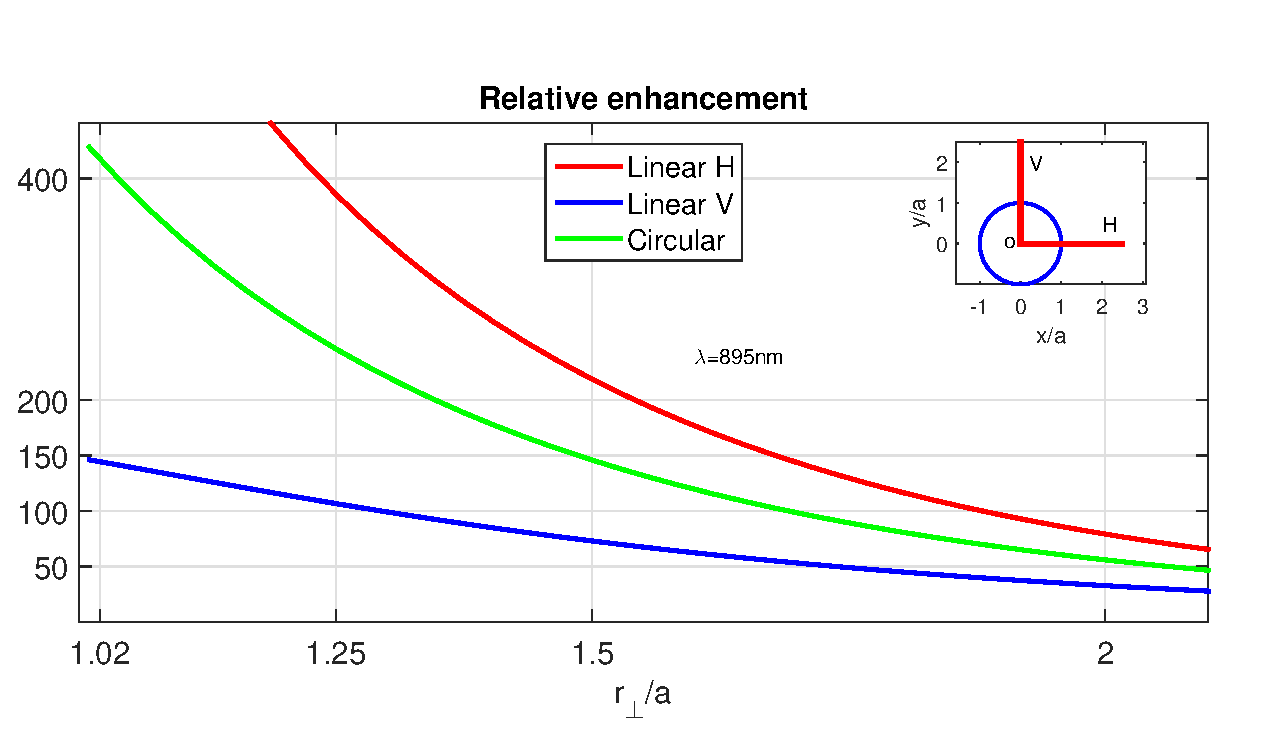
\includegraphics[width=0.95\linewidth]{../media/Figs/RelEnhancement}}
\caption[Relative atom-light coupling enhancement by using an optical nanofiber compared to a typical Gaussian beam trap.]{Relative enhancement of the atom-light coupling due to the use of a nanofiber compared to a typical Gaussian beam trap system. For the Gaussian beam system, an atom is placed at the center of the beam waist and the beam waist radius is $ 10\,\mu $m. Plotted are the relative phase shift or the modified decay rate as a function of the trapping radial position of the atom in the nanofiber system, where the atom is trapped along the $ H $ direction or the $ x $ axis. The $ H $ mode (red, top), $ V $ mode (blue, bottom) and the circular modes (green, middle) are plotted in the main figure. Inset indicates the coordinate of the atom position relative to the fiber (circle). The probe wavelength is $ \lambda=895 $ nm for comparison.}\label{fig:relenhancement}
\end{figure}

Figure~\ref{fig:relenhancement} plots the relative enhancement of the atom-light coupling due to the use of an optical nanofiber ($ a=225 $ nm) as a function of the atom's radial distance to the fiber axis. Different polarization states of the input light is studied in the figure while the atom is trapped along the $ x $ or $ H $ axis. The enhancement value is normalized to the case that the atom is probed at the center point of a Gaussian beam's waist with a typical waist radius $ w_0=10\,\mu $m. As shown, the nanofiber enhances the atom-light coupling by $ 30 $---$ 100 $ folds if the atom is trapped at $ r'_\perp=2a $, depending on the polarization state of the input light. If the atom is moved closer to the fiber surface, the enhancement can be further increased up to a few hundred folds. Note that both $ R $ and $ L $ circular modes of the nanofiber generate the same atom-light coupling strength in this rough model.

Similar results apply to the \SWG case. 


\bigskip
\textbf{The rotation angle on the \Poincare sphere:}
%\textcolor{red}{Diagrams for the configuration of setups...}
\begin{figure}[!tbp]
\centering\makebox[\textwidth]{
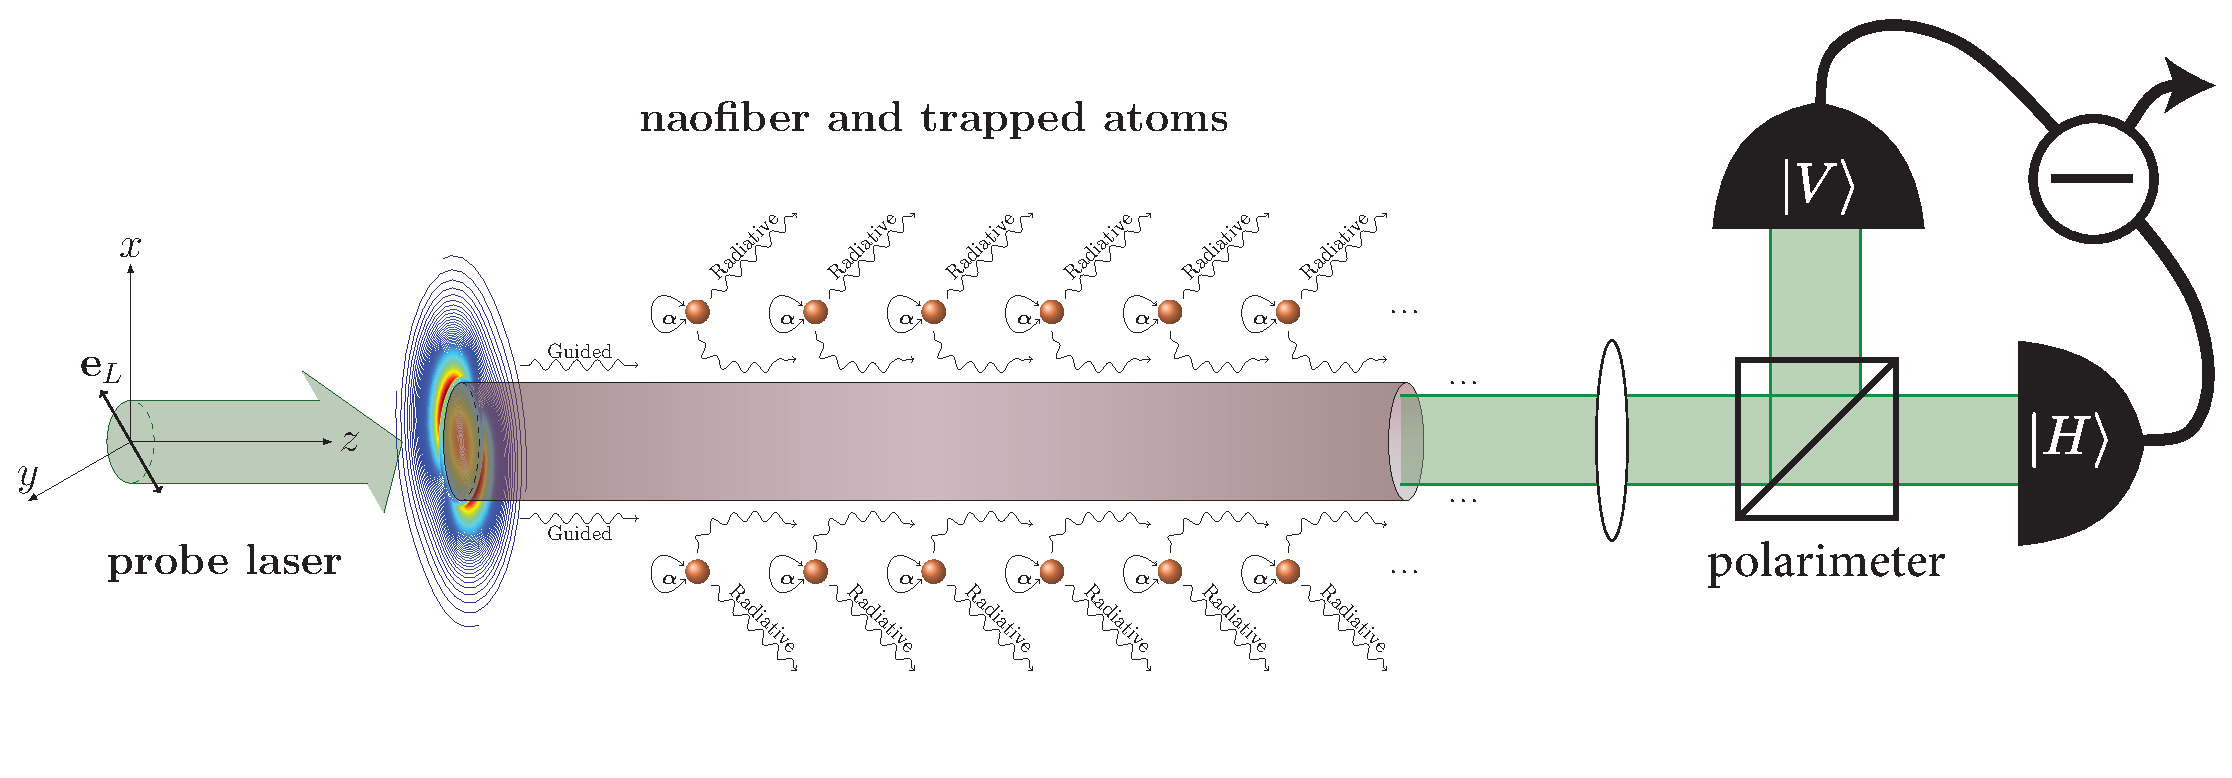
\includegraphics[width=12cm]{../media/Figs/BirefringenceMeasurement}}
\caption[Diagram depicting the polarization rotation measurement with an optical nanofiber.]{Diagram of polarization rotation measurement with an optical nanofiber (brown). The input light is initially polarized along the diagonal direction on the $ xy $ plane. 
The output polarization state is measured by the differential counting of the photon flux between the $ H $ and $ V $ linear polarization states. The rotated angle on the \Poincare sphere indicates a birefringence rotation of the guided light.}\label{fig:birefringencenanofibersetup}
\end{figure}

Suppose we launch a quasilinear $ D $ mode to the waveguide, which can be decomposed into two equal-power but orthogonal quasilinear modes, $H$ and $V$. 
Suppose we also place atoms along the major axis of the $H$ mode or the $ x $ axis. 
The atoms will feel both $ H $ and $ V $ modes in different strengths [see Figs.~\ref{fig:birefringencenanofibersetup} and~\ref{fig:Modes_Rot45HV_fiber}]. 
Since the local intensities of the $ H $ and $ V $ modes at the atom positions are different, there will be a differential phase shift between the output $ H $- and $ V $-polarized light components ($ \mathbf{E}_{H}(\br) $ and $ \mathbf{E}_{V}(\br) $), which generates a birefringence rotation on the \Poincare sphere. The rotation angle of the output light on the \Poincare sphere due to a scalar interaction with one atom can be given by
\begin{align}
\varphi &= \delta\phi_H-\delta\phi_V= 2\pi \frac{\omega_0}{v_g} \re[\alpha] \left[| \mathbf{u}_H(r'_{\!\perp})|^2- | \mathbf{u}_V(r'_{\!\perp})|^2 \right]\\
&= -\sigma_0\frac{c}{v_g}\frac{\Gamma_0}{4\Delta}\left[| \mathbf{u}_H(r'_{\!\perp})|^2- | \mathbf{u}_V(r'_{\!\perp})|^2 \right].\label{eq:birefringencerotang}
\end{align}

From Fig.~\ref{fig:relenhancement}, using the nanofiber, we find that the local $ H $ mode is usually $ 3 $---$ 4 $ folds stronger than the $ V $ mode along the $ x $ axis. 
This generates a strong birefringence effect even with a scalar polarizability of atoms, and is an otherwise unavailable resource for a free-space interface. 


%</waveguideinterface>



\appendix
% ########################### Apendix ##########################################
%<*polarizationstokesvectors>
\chapter{Polarization states of light and the Stokes vector representation}\label{chap:polarizationstokesvectors}
\section{Polarization states of light}

In free space, light is a transverse field. The polarization state of light\index{polarization} can be fully described by the amplitudes and relative phase of two orthogonal electric field components, $ \mathbf{E}_x $ and $ \mathbf{E}_y $:~\cite{Jackson1975}
\begin{subequations}
\begin{align}
\mathbf{E}_x(\br,t) &= \mathcal{E}_{x}\mathbf{e}_x e^{i(k_0z-\omega_0 t)},\\
\mathbf{E}_y(\br,t) &= \mathcal{E}_{y}\mathbf{e}_y e^{i(k_0z-\omega_0 t)},
\end{align}
\end{subequations}
where $ \mathcal{E}_{0x} $ and $ \mathcal{E}_{0y} $ are the complex amplitudes and $ \mathbf{e}_x $ and $ \mathbf{e}_y $ are the direction vectors along the $ x $- and $ y $-axes, respectively, in the transverse plane, perpendicular to the propagation direction along the $ z $ axis. 

A light is said to be \emph{linearly polarized}\index{polarization!linear polarization} if $\mathcal{E}_{x}$ and $ \mathcal{E}_{y} $ have the same phase. The polarization direction is set by the polarization angle $ \theta=\arctan(\mathcal{E}_{y}/\mathcal{E}_{x}) $ from the $ \mathbf{e}_x $ direction.
The polarization magnitude is defined to be $ E=\sqrt{\mathcal{E}_{x}^2+\mathcal{E}_{y}^2} $.

A light is said to be \emph{circularly polarized}\index{polarization!circular polarization} if $\mathcal{E}_{x}$ and $ \mathcal{E}_{y} $ have the same magnitude, but differ in phase by $ 90^\circ $. The wave can then be described by 
\begin{align}\label{eq:circularlightfield}
\mathbf{E}=E_0(\mathbf{e}_x \pm i\mathbf{e}_y)e^{i(k_0z-\omega_0 t)}
\end{align}
with $ E_0 $ the common real amplitude. Taking any point $ \br_0=(x_0,y_0,z_0) $ in space, the combined polarization vector $ \mathbf{e}_l(z_0)=(\mathbf{e}_x \pm i\mathbf{e}_y)e^{i(k_0z_0-\omega_0 t)} $ sweeps a complete circle at an angular frequency $ \omega_0 $.
Using the circular polarization basis vectors, $ \mathbf{e}_\pm $, defined by Eq.~\eqref{eq:epm}, the electric field can be rewrite as 
\begin{align} 
\mathbf{E}&=\sum_q \mathcal{E}_q\mathbf{e}_q=\mathcal{E}_+ \mathbf{e}_+ +\mathcal{E}_-\mathbf{e}_-\\
&=\mathcal{E}_L\mathbf{e}_++\mathcal{E}_R\mathbf{e}_- 
\end{align} 
with $ \mathcal{E}_q=\mathbf{e}_q^*\cdot \mathbf{E} $, and the left- and right-circular polarization amplitudes $ \mathcal{E}_L=\mathcal{E}_+ $ and $ \mathcal{E}_R=\mathcal{E}_- $, respectively. 
Note that the definition of \emph{left} and \emph{right} rotations in modern physics, including quantum mechanics, is different from that in traditional optics. In order to match the classical definitions of basic concepts with the quantum mechanical derivation in Chapter~\ref{chap:quantumdynamicsrepresentation}, we will primarily stick to the concept of \emph{helicity} in this chapter.

The Cartesian basis of the polarization measurement is usually called as the linear polarization basis (see Eq.~\eqref{eq:circularlightfield} for the circular polarization case). We can also use $ H $ (horizontal) and $ V $ (vertical) to label the $ x $ and $ y $ components of the field.
Alternatively, if the actual field is detected in the circular polarization basis, only one non-zero amplitude may be detected proportional to the circular polarization component 
\begin{align}
E_\pm(\br_0,t) &= \re\left[\mathbf{e}_\pm^* \cdot \mathbf{E}\right] = \re\left[\mathcal{E}_\pm \right].
\end{align}
I will label the polarization bases of positive and negative helicities with $ + $ and $- $ subscripts, respectively, in this dissertation. The choice of basis of polarization measurement can be operated by using beam splitters and proper wave planes in real experiments~\cite{Born1999Principles}.

If $\mathcal{E}_{x}$ and $ \mathcal{E}_{y} $ have different phases, the light is \emph{elliptically polarized}\index{polarization!elliptical polarization} in general. Represented in the circular polarization basis, the wave can be given by
\begin{align}
\mathbf{E}=(\mathcal{E}_+\mathbf{e}_+ + \mathcal{E}_-\mathbf{e}_-)e^{i(k_0z-\omega_0 t)},
\end{align}
where $ \mathcal{E}_\pm $ are complex amplitudes, and $ \mathrm{angle}\left(\mathcal{E}_+\right)$ may not equal to $\mathrm{angle}\left(\mathcal{E}_-\right) $. 
When $ \mathcal{E}_+ $ and $ \mathcal{E}_- $ have different magnitudes yet the same phase, the light is elliptically polarized with the $ \mathbf{E} $ vector traced as an ellipse defined by the principle axes pointing along $ \mathbf{e}_x $ and $ \mathbf{e}_y $ directions~\cite{Jackson1975}. The semimajor and semiminor axes of the ellipse have a ratio of $ |(1+r)/(1-r)| $, where $ r=\mathcal{E}_+/\mathcal{E}_- $. 
When the two complex amplitudes in the circular polarization basis have a phase difference, $ \phi $, or $ \mathcal{E}_+/\mathcal{E}_-=re^{i\phi} $, then the traced ellipse of the $ \mathcal{E} $ vector has its principal axes rotated by an angle $ \phi/2 $ from the $ \mathbf{e}_x $ and $ \mathbf{e}_y $ axes. 
The real parameter $ r $ is the ellipticity\index{polarization!ellipticity} of the ellipse of the $ \mathbf{E} $ vector trace. For $ r=\pm 1 $, we recover the linear polarization case. 

\section{Stokes vectors and polarization measurement}

To help visualize the polarization state of the light, we rewrite the field amplitudes\footnote{In the terminology of modern physics, they are also the components of Jones vectors defining a polarized light~\cite{Born1999Principles}.} in the linear and circular polarization bases by
\begin{align}
\mathcal{E}_x &= E_x e^{i\delta_x},\quad & \mathcal{E}_y &= E_y e^{i\delta_y},\\
\mathcal{E}_+ &= E_+ e^{i\delta_+},\quad & \mathcal{E}_- &= E_- e^{i\delta_-},
\end{align} 
where $ E_{x/y} $, $ E_\pm  $, $ \delta_{x/y} $ and $ \delta_\pm $ are all real parameters. Traditionally, the Stokes vector $ \mathbf{S}=(S_0,S_1,S_2,S_3) $ is usually employed in literature to uniquely project the polarization state of the light onto the famous \Poincare sphere\cite{Born1999Principles} (see Fig.\ref{fig:Poincaresphere}). In terms of the linear polarization basis $ (\mathbf{e}_x,\mathbf{e}_y) $, the Stokes vector components are~\cite{Born1999Principles}
\begin{subequations}\label{eq:S_xybasis}
\begin{align}
S_0 &= |\mathbf{e}_x\cdot \mathbf{E}|^2+|\mathbf{e}_y\cdot \mathbf{E}|^2 =E_x^2+E_y^2\\
S_1 &= |\mathbf{e}_x\cdot \mathbf{E}|^2-|\mathbf{e}_y\cdot \mathbf{E}|^2 =E_x^2-E_y^2\\
S_2 &= 2\re\left[ (\mathbf{e}_x\cdot \mathbf{E})^*(\mathbf{e}_y\cdot \mathbf{E})\right] =2E_xE_y\cos(\delta_y-\delta_x)\label{eq:S2_xybasis}\\
S_3 &= 2\im\left[ (\mathbf{e}_x\cdot \mathbf{E})^*(\mathbf{e}_y\cdot \mathbf{E})\right] =2E_xE_y\sin(\delta_y-\delta_x)
\end{align}
\end{subequations}

Similarly, in the circular polarization basis $ (\mathbf{e}_+,\mathbf{e}_-) $, the Stokes vector components can be given by
\begin{subequations}\label{eq:S_circularbasis}
\begin{align}
S_0 &= |\mathbf{e}_+^*\cdot \mathbf{E}|^2+|\mathbf{e}_-^*\cdot \mathbf{E}|^2 =E_+^2+E_-^2\\
S_1 &= 2\re\left[ (\mathbf{e}_+^*\cdot \mathbf{E})^*(\mathbf{e}_-^*\cdot \mathbf{E})\right] = 2E_+E_-\cos(\delta_--\delta_+)\\
S_2 &= 2\im\left[ (\mathbf{e}_+^*\cdot \mathbf{E})^*(\mathbf{e}_-^*\cdot \mathbf{E})\right] =2E_+E_-\sin(\delta_--\delta_+)\\
S_3 &= |\mathbf{e}_+^*\cdot \mathbf{E}|^2-|\mathbf{e}_-^*\cdot \mathbf{E}|^2 =E_+^2-E_-^2 %=E_L^2-E_R^2
\end{align}
\end{subequations}
 %(\qxd{Note: should the $S_3$ be $ E_R^2-E_L^2 $ instead?})
The Stokes vector components are independent from the choice of basis. 
One can choose another linear polarization basis, namely, the diagonal polarization basis $ (\mathbf{e}_D,\mathbf{e}_{\thickbar{D}}) $ defined by Eq.~\eqref{eq:eDeDbar}. 
The $ \mathbf{E} $ vector can then be written as  \begin{align}
\mathbf{E} = \mathcal{E}_D\mathbf{e}_D + \mathcal{E}_{\thickbar{D}}\mathbf{e}_{\thickbar{D}}=E_De^{i\delta_D}\mathbf{e}_D + E_{\thickbar{D}}e^{i\delta_{\thickbar{D}}}\mathbf{e}_{\thickbar{D}} .\label{eq:E_Dbasis}
\end{align}
Plugging Eqs.~\eqref{eq:eDeDbar} and~\eqref{eq:E_Dbasis} into Eq.~\eqref{eq:S2_xybasis}, one can find that in the diagonal polarization basis
\begin{align}\label{eq:S2_Dbasis}
S_2 = E_D^2-E_{\thickbar{D}}^2.
\end{align}
%\qxd{(Comment: why not $ E_{\thickbar{D}}^2-E_{D}^2 $?)}
Based on the expressions of Stokes vectors in different bases or Eqs.~(\ref{eq:S_xybasis},~\ref{eq:S_circularbasis} and~\ref{eq:S2_Dbasis}), we can find the relation between those Stokes vector components and the intensity of field components $ E_i^2 $ in different bases as follows:
\begin{subequations}\label{eq:S_intensitydiff_appendix}
\begin{align}
S_0 &= E_H^2+E_V^2 = E_+^2+E_-^2 = E_D^2+E_{\thickbar{D}}^2,\\
S_1 &= E_H^2-E_V^2,\\
S_2 &= E_D^2-E_{\thickbar{D}}^2,\\
S_3 &= E_+^2-E_-^2. %=E_L^2-E_R^2
\end{align}
\end{subequations}
Above, we have replaced $ x\rightarrow H $ and $ y\rightarrow V $.

%</polarizationstokesvectors>

%<*guidedunguidedmodes>
\chapter{Guided and unguided modes of a waveguide}\label{chap:guidedunguidedmodes}
Below, we sketch out the condition to divide the guided and radiation modes using an analogy to the \sch equation and based on the total internal reflection condition.

\section{Wave equations as a scattering problem in analogy}
If we want to fully calculate the eigenmodes of a waveguide, we need to consider both the electric and magnetic fields, the spatial parts of which are governed by the wave equations
\begin{align}\label{EBz}
\left(\nabla^2 +k^2 \varepsilon(\br_{\perp})\right) \begin{pmatrix}
\mathcal{E}_z(\br)\\
\mathcal{B}_z(\br)
\end{pmatrix} = 0,
\end{align}
where $ \varepsilon=n^2 $ is the permittivity of the medium and $ k $ is the wavenumber of the modes. The equation above is derived from the \emph{Maxwell-Helmholtz equation}\index{Maxwell-Helmholtz equation}, for example,
\begin{align}
\left[ -\nabla\times\nabla\times+\frac{\omega^2}{c^2}n^2(\br) \right] \boldsymbol{\mathcal{E}}(\br) &=0. \label{MaxwellHelmholtz0},
\end{align}
for the electric field part.
Notice that we only concentrate on the $ z $-component of the fields since all the other components can be expressed in terms of the $ z $-components. (See a detailed derivations in Appendix~\ref{MWE:components} in the cylindrical coordinate system). 

We use the ansatz
\begin{align}
\mathcal{E}_z (r_\perp, \phi, z) &= \psi(r_\perp,\phi) e^{i\beta z},\\
\mathcal{B}_z (r_\perp,\phi,z) &= \zeta(r_\perp,\phi) e^{i\beta z}.
\end{align}
Substituting the above into Eq.~\ref{EBz}, we obtain
\begin{align}\label{psizeta}
\left(\nabla^2_\perp +(k^2 \varepsilon(\br_{\perp})-\beta^2 )\right) \begin{pmatrix}
\psi(r_\perp,\phi)\\
\zeta(r_\perp,\phi)
\end{pmatrix} = 0.
\end{align}
Now, the problem of solving a three dimensional wave equation for $ \boldsymbol{\mathcal{E}} (r_\perp, \phi, z) $ 
and $ \boldsymbol{\mathcal{B}} (r_\perp, \phi, z)$ turns into a problem of solving a two-dimension differential 
(mode) equation for $ \psi(r_\perp,\phi) $ and $ \zeta(r_\perp,\phi) $. 

There are two special cases for the modes. If $ \psi=0 $ is constant, which means there is no $ z $-component of the electrical field, then the propagating mode is called a TE mode\index{mode!TE mode}. Similarly, if $ \zeta=0 $ is constant, which corresponds to zero magnetic $ z $-component, 
then this mode is called a TM mode\index{mode!TM mode}. However, in many waveguide geometries including the nanofiber case with a cylindrical symmetry, the modes cannot be grouped into TE and TM guided waves. In general, the modes with 
both nonzero electrical and magnetic  $ z $-components are known as EH and HE hybrid 
modes\index{mode!HE mode}~\cite{Snyder1983Optical}--the second letter in the names indicates the field with a dominant longitudinal component.

We focus on the electrical part for now. The magnetic field can be solved similarly. Eq.~\ref{psizeta} gives
\begin{align}\label{eigenpsi}
[\nabla^2_\perp + k^2\varepsilon(r_\perp)] \psi(r_\perp, \phi) = \beta^2\psi(r_\perp,\phi).
\end{align}
Compared to the time-independent \sch equation
\begin{align}
\left[\frac{\hat{P}^2}{2m}+V(\hat{\mathbf{r}}_\perp) \right] \psi(\br_\perp)&= E\psi(\br_\perp),\\
\text{or}\quad \left[ \nabla^2_\perp -V(r_\perp) \right] \psi (r_\perp, \phi) &= -E\psi(r_\perp,\phi),
\end{align}
we can conclude that the mode equation (Eq.~\ref{eigenpsi}) is basically an eigenvalue equation for the \sch wavefunctions if we make the replacement
\begin{align}
V_{ef\!f}=-k^2\varepsilon(\br\!_\perp) &\sim V(\br\!_\perp),\\
-\beta^2 &\sim E.
\end{align}
With these analogies, we find that the guided modes dictated by the wave equation should correspond to the bound eigenstates of the trapping potential problem obeying the \sch equation; likewise, the radiation modes of the wave equation correspond to unbound states in the scattering problem following the \sch equation. In details, for the time-independent \sch problem, if $ 0<E\leq V $, then the eigenstates are bounded and have discrete solutions with respect to $ E $; if $ E>V $, then the resulting states is unbound and have continuous solutions of energy. For the waveguide's eigenmodes, similarly, we can also use the relative position of $ V_{ef\!f} $ and $ -\beta^2 $ to classify the bound and radiation modes. 

Let us consider the concrete case of a nanofiber with step-function-like permittivity as a function of $ r_\perp $. The analogy of trapping potentials of the wave equation is illustrated in Fig.~\ref{Figs/scatteredmode}. In the regime $ n_2k<\beta<n_1k $, the eigenmodes have discrete solutions with respect to $ \beta $, which yield $ \beta=\beta_0 $ for a single-mode fiber; in the $ 0<\beta<n_2k $ regime, the eigenmode solutions are continuous with respect to $ \beta $. Similar result applies to the \SWG case. 

%\scalefig{Figs/scatteredmode}{0.8}{Bound and unbound states for the nanofiber eigenvalue 
%problem. $ \varepsilon(r\!_\perp)=\varepsilon_{f} =n_1^2$ if $ r_\perp < a $; otherwise, $\varepsilon
%(r\!_\perp) =1 $. The parameter $ a $ is the radium of the nanofiber. } 

\begin{figure}[!tbp]
\centering\makebox[\textwidth]{
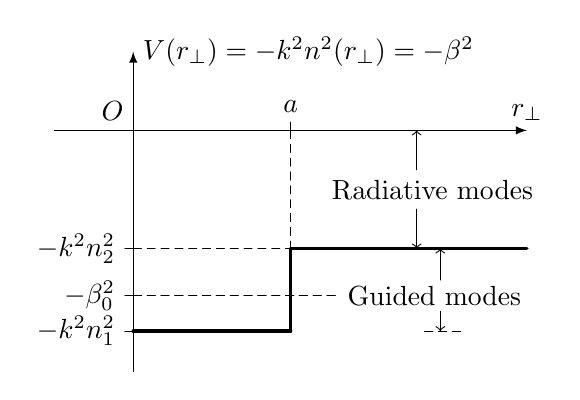
\begin{tikzpicture}[scale=1,cap=round]
% Configurable parameters
\def\k{1.5cm}
\def\eps{1.5*1.7cm}
\def\betasq{1.5*1.4cm}
\def\a{2cm}
\def\maxr{5cm}

% Styles
\tikzstyle{axes}=[arrows={-latex}]
\tikzstyle{auxline}=[densely dashed]
\tikzstyle{important line}=[very thick]

% Coordinates and points.
\coordinate (O) at (0,0);	% Origin.
\coordinate (A) at (\a,0);	% The surface distance to the axis of the fiber.
\coordinate (B) at (0,-\eps);	% -k^2\epsilon at the center of the fiber.
\coordinate (C) at (\a,-\eps);	% -k^2\epsilon on the surface of the fiber.
\coordinate (D) at (0,-\betasq);	% -\beta^2 point at the center of the fiber.
\coordinate (E) at (\a*1.3,-\betasq);	% -\beta^2 point at the end of the maximum r.
\coordinate (F) at (0,-\k);	% -k^2 point at the center of fiber.
\coordinate (G) at (\a,-\k); 	% -k^2 point on the surface of the fiber.
\coordinate (H) at (\maxr,-\k); 	% -k^2 point at the end of r.

% The graphic
 % help grid
% \draw[style=help lines,step=0.5cm] (-2.0,-2.0) grid (2.0,2.0);
  
% Draw axes and marks.
\draw [axes] (-1cm, 0) -- (\maxr,0) node [above] {$r_{\perp}$};
\draw [axes] (0, -1.2*\eps) -- (0, 1.0cm) node [right] {$V(r_{\perp})=-k^2n^2(r_{\perp})=-\beta^2$};
\draw (O) node [above left] {$O$};
\draw[thin] (A) -- (\a,3pt) node[anchor=south] {$a$}; 
\draw (B) -- (-3pt,-\eps) node[anchor=east] {$-k^2n_1^2$};
\draw (D) -- (-3pt,-\betasq) node[anchor=east] {$-\beta_0^2$};
\draw (F) -- (-3pt,-\k) node[anchor=east] {$-k^2n_2^2$};

% Draw potential lines.
\draw[important line] (B) -- (C);
\draw[important line] (C) -- (G);
\draw[important line] (G) -- (H);
\draw[auxline] (D) -- (E) node[right] {Guided modes};
\draw[auxline,very thin] (F) -- (G);
\draw[auxline,very thin] (A) -- (G);

% Other labels and auxlines.
%\draw[<->] (\a*1.25,0) -- (\a*1.25,-\k) node[midway,right] {Scattered modes};
\draw (\a*1.2,-\k/2) node[right] {Radiative modes};
\draw[<-] (\a*1.8,0) -- (\a*1.8,-0.5cm);
\draw[->] (\a*1.8,-1cm) -- (\a*1.8,-\k);
\draw[<-] (\a*1.95,-\k) -- (\a*1.95,-\k-0.4cm);
\draw[->] (\a*1.95,-\k-0.8cm) -- (\a*1.95,-\eps);
\draw[auxline] (\a*1.85,-\eps) -- (\a*2.08,-\eps);
\end{tikzpicture}
}
\caption[Trapping potential analogy of the bound and unguided modes of a nanofiber.]{Bound and unbound states for the fiber eigenvalue problem. $ \varepsilon(r\!_\perp)=\varepsilon_{f} =n_1^2$ if $ r_\perp < a $; otherwise, $\varepsilon(r\!_\perp) =1 $. The parameter $ a $ is the radius of the nanofiber.}
\label{Figs/scatteredmode}
\end{figure}

\section{Categorizing eigenmodes based on the total internal reflection condition}
The division of guided and radiation modes based on the value of $ \beta $ can also be roughly understood in the perspective of geometric optics as elucidated in Fig.~\ref{fig:Fibermodes}. We regard $ \beta $ as the $ z $-projected wave number of a wave vector of the light ray on the $ \vec{k} $ direction. If the ray is incident in an angle that satisfies the total internal reflection condition (in our case, $ k_0<\beta<n_1k_0 $ with $ n_2=1 $), the corresponding modes are guided; otherwise, the modes are unguided with the light leaking out and decaying along $ z $.

\begin{figure}[!tbp]
\centering\makebox[\textwidth]{
\begin{tikzpicture}[scale=1,cap=round]
% Configurable parameters
\def\fiberrad{1cm}	% Radius of the nanofiber.
\def\comprad{0.45cm}	% Compressed radius of the nanofiber in the view angle.
\def\fiberleftx{0}	% The x-coordiante of the center of the left surface of the fiber.
\def\fiberlefty{0}	% The y-coordiante of the center of the left surface of the fiber.
\def\fiberlength{6.6cm} % The length of the fiber.

% Styles
\tikzstyle{axes}=[arrows={-latex}]
\tikzstyle{auxline}=[densely dashed]
\tikzstyle{important line}=[thick]
\tikzstyle{dot}=[circle,inner sep=1pt,fill,label={#1},name=#1]

% Coordinates and points.
\coordinate (O) at (0,0);	% Origin.
\coordinate (LO) at (\fiberleftx,\fiberlefty); % Center of the left-side surface of the nanofiber.
\coordinate (RO) at (\fiberleftx+\fiberlength,\fiberlefty); % Center of the right-side surface
\coordinate (A) at ({\fiberleftx},{\fiberlefty+\fiberrad});	% Top-left point of the nanofiber.
\coordinate (B) at ({\fiberleftx+\fiberlength},{\fiberlefty+\fiberrad});	% Top-right point of the nanofiber.
\coordinate (C) at ({\fiberleftx+\fiberlength},{\fiberlefty-\fiberrad});	% Bottom-right point of the fiber.
\coordinate (D) at ({\fiberleftx},{\fiberlefty-\fiberrad});	% Bottom-left point of the nanofiber.

% The graph.
% help grid
% \draw[style=help lines,step=0.5cm] (-2.0,-2.0) grid (2.0,2.0);

% Draw the fiber.
\begin{scope} 
    % Outer edge.
    %\fill[left color=purple!50!black,right color=purple!50!black,middle 
%color=purple!50,shading=axis,opacity=0.25] (A) -- (B) arc (90:270:{\comprad} and {\fiberrad}) -- (D) arc 
%(270:90:{\comprad} and {\fiberrad});
    % Right-side surface.
    %\fill[top color=purple!90!,bottom color=purple!2,middle color=purple!30,shading=axis,opacity=0.25] 
%(RO) circle [x radius={\comprad}, y radius = {\fiberrad}];
    % Draw lines of all edges.
    \draw (A) -- (B);
    \draw  (RO) circle [x radius = {\comprad}, y radius =  {\fiberrad}];
    \draw (C) -- (D) arc (270:90:{\comprad} and {\fiberrad}); 
    \draw[densely dashed] (A) arc (90:-90:{\comprad} and {\fiberrad});
\end{scope}

% Draw the guide mode wave vector and propagation lines.
% First part of the ray: up-solid line.
\draw[red] (O)--(2.0*\fiberrad,\fiberrad);
%\draw[red,decoration={ markings,  % This schema allows for fine-tuning the arrows.
%      mark=at position 0.5 with {\arrow{latex'}}, 
%      mark=at position 0.82 with {\arrow{latex'}}},postaction={decorate}] (O) -- (2.0*\fiberrad,\fiberrad)-- (6.0*\fiberrad,-\fiberrad);
% The penetration part of ray: dashed line.
\draw[red,densely dotted] (2.0*\fiberrad,\fiberrad) -- (2.3*\fiberrad,1.1732*\fiberrad) -- (2.6*\fiberrad,\fiberrad);
% The reflected part: solid downarrow.
\draw[red,decoration={ markings,  % This schema allows for fine-tuning the arrows.
      mark=at position 0.2 with {\arrow{latex'}}, 
      mark=at position 0.6 with {\arrow{latex'}}},postaction={decorate}] (2.6*\fiberrad,\fiberrad)-- (6.6*\fiberrad,-\fiberrad);
% The ruler part.
\draw[important line,-latex'] (O) --(27:1) node[below,xshift=8,yshift=5] {$ \vec{k} $};
\draw[auxline] (27:1) -- ({cos(27)},-1.5)  node [below] {$\beta_0$};

% Draw radiation modes.
% Radiation ray 1:
\draw[blue,decoration={ markings,  % This schema allows for fine-tuning the arrows. 
      mark=at position 0.95 with {\arrow{latex'}}},postaction={decorate}] (O) -- (0.5,\fiberrad) -- (1.5,\fiberrad*1.1);
\draw[-latex'] (O)--(63.5:1);
\draw[auxline] (63.5:1) -- ({cos(63.5)},-2);
% Radiation ray 2:
\draw[blue,decoration={ markings,  % This schema allows for fine-tuning the arrows. 
      mark=at position 0.95 with {\arrow{latex'}}},postaction={decorate}] (O) -- (0.4,\fiberrad) -- (1.4,\fiberrad*1.4);
\draw[-latex'] (O)--(68.5:1);
\draw[auxline] (68.5:1) -- ({cos(68.5)},-2);
% Radiation ray 3:
\draw[blue,decoration={ markings,  % This schema allows for fine-tuning the arrows. 
      mark=at position 0.95 with {\arrow{latex'}}},postaction={decorate}] (O) -- (0.25,\fiberrad) -- (0.9,\fiberrad*1.9);
\draw[-latex'] (O)--(76:1);
\draw[auxline] (76:1) -- ({cos(76)},-2);
% Radiation ray 3:
\draw[blue,decoration={ markings,  % This schema allows for fine-tuning the arrows. 
      mark=at position 0.95 with {\arrow{latex'}}},postaction={decorate}] (O)-- (0,2*\fiberrad);
\draw[-latex'] (O) -- (0,\fiberrad);
% Draw dots inbetween.
\draw[dotted] ([shift=(26:1)] 0.2,1.0*\fiberrad) arc (26:45:1);
\draw[dotted] ([shift=(60:1)] 0.1,1.0*\fiberrad) arc (60:89:1);

% Labels and denotes.
\draw (O) node[dot] {};
\draw (O) node[left] {O};
\draw[auxline,-latex] (O) -- (\fiberlength*1.0,0) node [above] {$ z $};	% Z axis line.
\draw[auxline] (0,\fiberrad) -- (0,-2);
\draw[important line,-latex] (0,-2) node[left] {$ 0 $}--(2.5,-2) node[right] {$ k_z $};% kz axis.
\draw (0,-2) -- (0,-2.08);
\draw (0.5,-2) -- (0.5,-2.08) node [anchor=north] {$k_0$};
\draw ({cos(27)},-2) -- ({cos(27)},-2.08);
\draw (1.1,-2) -- (1.1,-2.08) node [below right,xshift=-5] {$k_0n_1$};
\draw (3.35,-0.5) node[red] {Guided modes};	% Guided modes label.
\draw (2.7,1.7*\fiberrad) node[blue] {Radiative modes};	% Radiative modes label.
\end{tikzpicture}
}
\caption[Fiber modes classified through the $ z $-component of the wave vector, $ \beta $.]{Fiber modes classified through the $ z $-component of the wave vector, $ \beta $. We have assumed $ n_2=1 $ for the vacuum clad. From the diagram, we define $ \beta $ is the $ z $-projection of $ \vec{k} $, that is $ \beta=k\cos\theta $, where $ k $ is the length of the wave vector following the ray-trace of the light propagating in all directions, and $ \theta $ is the angle of the ray of light to the $ z $ axis. We see that when $ \theta $ is small or $ \beta $ is longer than some value, the light can satisfy the total internal reflection condition and hence the corresponding mode solution can be guided through the fiber; if $ \theta $ is large or $ \beta $ is small, then the light cannot satisfy the total internal reflection condition, and hence the corresponding modes are unguided or radiation leaking out of the fiber.}
\label{fig:Fibermodes}
\end{figure}
%</guidedunguidedmodes>

%<*eigenmodes>

\chapter{Fundamental eigenmodes of an optical nanofiber}\label{chap:fibereigenmodes}

In this appendix chapter, we will provide some details on solving the eigenmodes of the nanofiber starting from the homogeneous wave equation, Eq.~\ref{EBz}, and will give the formulas for mode normalization based on power and the eigenmode normalization condition. At the end of this chapter, we will also derive the formulas for calculating the group velocity of the \HE mode of the nanofiber.

First, starting form the operator
\begin{align}
\nabla^2 \!_\perp = \frac{1}{r_{\!\perp}}\pp{}{r\!_\perp}\! \left(r\!_\perp \pp{}{r\!_\perp} \right) + 
\frac{1}{r_\perp^2} \spp{}{\phi},
\end{align}
and the symmetry of the fiber,  we can separate the mode function by
\begin{align}
\psi(r\!_\perp,\phi)=\mathcal{E}_{z,\beta m}(r\!_\perp)e^{im\phi},
\end{align} 
and hence
\begin{align}
\mathcal{E}_z(r\!_\perp,\phi,z) = \mathcal{E}_{z,\beta m}(r\!_\perp)e^{i(m\phi+\beta z)},
\end{align}
where $ \mathcal{E}_{z,\beta m}(r\!_\perp) $ satisfies the Bessel's equation
\begin{align}
\left[ \spp{}{r\!_\perp}+ \frac{1}{r_{\!\perp}}\pp{}{r\!_\perp}- 
\frac{m^2}{r^2\!_\perp} + (k^2\varepsilon(r\!_\perp)-\beta^2) \right] 
\mathcal{E}_{z,\beta m}(r\!\!_\perp)=0
\end{align}
with 
\begin{align}
\varepsilon(r\!\!_\perp) = 
\begin{cases}
1, & r\!_\perp>a\\
\varepsilon_f, & r\!_\perp\leq a.
\end{cases}
\end{align}
The general solution for $ \mathcal{E}_{z,\beta m}(r\!\!_\perp) $ can be given in three cases 
corresponding to different 
boundary conditions
\begin{align}
\mathcal{E}_{z,\beta m}(r\!\!_\perp) = \begin{cases}
AJ_m(qr\!\!_\perp) + B Y_m(qr\!_\perp)&\rightarrow J_m(\theta)\sim \cos\theta,\, Y_m(\theta)\sim 
\sin\theta.\\
CI_m(qr\!_\perp) + DK_m(qr\!_\perp) & \rightarrow I_m(\theta) \sim e^\theta,\, K_m(\theta) \sim 
e^{-\theta}.\\
EH_m^{(\!1\!)}(qr\!_\perp) \!+\! FH_m^{(\!2\!)}(qr\!_\perp ) & \rightarrow H_m^{(\!1\!)} (\theta) \! \sim \! 
e^{i\theta},\, 
H_m^{(\!2\!)}(\theta)\!\sim\! e^{\!-i\theta}.
\end{cases}
\end{align}
$J_m$ and $Y_m$ are the $m^{th}$ Bessel functions of the first and second kind.
$I_m$ and $K_m$ are the $m^{th}$ modified Bessel functions of the first and second kind.
$H_m^{(1)}$ and $H_m^{(2)}$ are the $m^{th}$ Hankel functions of the first and second kind.
The positive parameter $ 1/q $ is the characteristic decay length corresponding to $ 1/h_{11} $ and $ 
1/q_{11} $ 
in the $\text{HE}_{11}$ mode expression. Using the symmetric and convergent condition at $ 
r\!_\perp=0\,\text{and}\, \infty $, as for guided modes, for example, if $k< \beta\leq 
k\sqrt{\varepsilon_f}$,
\begin{align}
\left\{
 \begin{array}{lcll}
	r\!_\perp \leq a, & \mathcal{E}_{z,\beta m}(r\!_\perp )\!=\! AJ_m(h r\!_\perp), & h \!=\! 
	\sqrt{k^2\varepsilon_f-\beta^2}\! >\! 0;\\
	r\!_\perp > a, & \mathcal{E}_{z,\beta m}(r\!_\perp )\!=\!DK_m(q r\!_\perp), & q\!=\! 
	\sqrt{\beta^2-k^2}>0.
 \end{array}\right.
\end{align}
Both $ \beta $ and $ h $ are discrete for guided modes. 
For unguided modes, $ 0\leq \beta< k $, similarly, 
\begin{align}
\left\{
 \begin{array}{lcll}
	r\!_\perp \leq a, & \mathcal{E}_{z,\beta m}(r\!_\perp )\!=\! AJ_m(h r\!_\perp), & h \!=\! 
	\sqrt{k^2\varepsilon_f-\beta^2}\! >\! 0;\\
	r\!_\perp > a, & \mathcal{E}_{z,\beta m}(r\!_\perp )\!=\!EH_m^{(\!1\!)}(p r\!_\perp\!), & p\!\!=\!\! 
	\sqrt{k^2-\beta^2}>0.
 \end{array}\right.
\end{align}
Both $ \beta $ and $ p $ are continuous. 
%\textcolor{red}{(Double check the general solutions and the consistence with Eq.~\ref{ET0Rexpand}.)}
%Notice that Ref.\cite{Snyder1983} used $ J_m(hr\!_\perp)\cos m\phi $ and $ 
%(J_m(pr\!_\perp)+CH_m^{(\!1\!)})\cos m\phi $ as the basis for the general solution of $ e $ and $ o $ 
%light 
%of the radiation modes, and summed them up. They are equivalent to the solution here.  

At a given frequency, $\omega = c k$, the magnitudes of the longitudinal and transverse wave vectors for a guided mode are related by $n^2 k^2 = \beta^2 + k_\perp^2$.  
The positive propagation constant, $\beta \equiv \beta(\omega)$, is determined from the eigenvalue equation that results from enforcing physical boundary conditions at the fiber surface~\cite{Snyder1983Optical},
	\begin{align}\label{eq:eigenfunctionbeta}
		\frac{J_0(ha)}{ha J_1(ha)} &= - \frac{n_1^2+n_2^2}{2n_1^2} \frac{K'_1(qa)}{qa K_1(qa)} + \frac{1}{h^2 a^2} \nn\\
		&\quad - \bigg[ \bigg(\frac{n_1^2 - n_2^2}{2 n_1^2} \frac{K'_1(qa)}{qa K_1(qa)} \bigg)^2  + \frac{\beta^2}{n^2_1 k^2} \bigg(\frac{1}{q^2a^2} + \frac{1}{h^2a^2} \bigg)^2 \bigg]^{1/2}.
	\end{align}
Above, $f'(x)$ indicates a derivative with respect to the argument $x$.
Inside the nanofiber the transverse wavevector is real, $k_\perp = q$, where $q=\sqrt{\beta^2- n_2^2k^2}$, and outside the nanofiber it is purely imaginary, $k_\perp = i h$, where $h=\sqrt{n_1^2 k^2 - \beta^2}$.  

If $ \beta $ is a pure imaginary number, the field will have an exponential decay amplitude on the $ z $ direction, and will spread the energy away from the fiber axis. Reference~\cite{Snyder1983Optical} denotes the modes with pure imaginary $ \beta $ as evanescent modes. If $ \beta $ has both real and imaginary parts, the modes are denoted as leaky modes, which are combinations of radiation modes and evanescent modes. Except for the case that the incident light is highly directed at the complementary critical angle $ \theta_c $ of geometric optics, the radiation modes part alone can propagate for a long distance along the fiber axis. In our nanofiber system, we only consider the bound and radiation modes. The ranges of some waveguide parameters are given in Table~\ref{tab:fiberparameters}. 
In the table, we have defined the normalized wave number\cite{Snyder1983Optical}, or 
$V$-number\index{V-number@$V$-number} 
of a fiber as $V  = 
k_f a \mathrm{NA}$.  Here $k_f=\frac{2\pi}{\lambda}$, is the free space wave number, $a$ is the radius 
of the core of the fiber, and $\mathrm{NA}$ is the numerical aperture\index{numerical aperture} of 
the fiber, $\mathrm{NA} = 
(n_1^2 - n_2^2)^{1/2} = n_1(2\Delta)^{1/2}$, with profile height 
parameter\index{profile height parameter} 
$\Delta =\frac{1}{2}(1-n_2^2/n_1^2)\approx (n_1-n_2)/n_1$.  For 
different modes labeled with $ j $, we always have $V_j^2=a^2(h_j^2+q_j^2)$ and $ \lambda\beta_j/2\pi $ is a mode invariance.  The TE and TM modes have non-vanishing cut-off 
frequencies, as $ a\rightarrow 0 $.  The cutoff frequency is found from $V = a\omega (\Delta)^{1/2}/c =2.405$ for silicon fiber.  
Only the lowest HE mode, $\mathrm{HE}_{11}$, has no cutoff frequency as $ a\rightarrow 0 $.  For $0 < V < 2.405$, which is the case of the nanofiber we are studying, it is the only mode that propagates in the 
fiber. For fixed $ \varepsilon_f $, in the range that $ 0\leq \beta \leq 
k\sqrt{\varepsilon_f} $, we can distinguish the radiation and guided mode as follows:
\begin{align}
\begin{cases}
0\leq \beta < k, &\rightarrow \text{\emph{unbound/radiation modes;}}\\
k< \beta \leq k \sqrt{\varepsilon_f}, &\rightarrow \exists \text{ a},\, \text{HE}_{11}\, \text{\emph{is the only 
guided mode.}}
\end{cases}
\end{align}


\begin{minipage}{0.97\textwidth}
\centering
\captionof{table}{Ranges of fiber parameters for different modes. } \label{tab:fiberparameters} 
\begin{tabular}{|l|c|c|c|}
\hline  & $\beta$ & $h$ & $p$ \\ 
\hline Bound modes & $k<\beta_j \leq k\sqrt{\varepsilon_f} $ & $ 0\leq h_j<V/a $ & $ p^r_j=0,\, p^i_j>0 $ \\ 
\hline Radiation modes & $0\leq \beta<k$ & $V/a < h\leq k\sqrt{\varepsilon_f}$ & $0<p\leq k $\\ 
\hline Evanescent modes & $ \beta^r=0,\, \beta^i>0 $ & $ k\sqrt{\varepsilon_f} < h $ & $ k<p $ \\ 
\hline 
\end{tabular} 
\par
\bigskip
%The caption:
Superscripts $ r $ and $ i $ denote real and imaginary parts. Subscripts $ j $ denotes the discrete indeces for guided modes. Adapted from Ref.~\cite{Snyder1983Optical} P.P.516 Table 25-1. This can also be understood in geometric optics as shown in Fig.(\ref{fig:Fibermodes}).
\end{minipage}
\bigskip



Due to the symmetry of equations, we also have
\begin{align}
\mathcal{B}_z(r\!_\perp,\phi,z) = \mathcal{B}_{z,\beta m}(r\!_\perp)e^{i(m\phi+\beta z)},
\end{align}
where $  \mathcal{B}_{z,\beta m}(r\!_\perp) $ satisfies the same Bessel's equation as above.  

In the case of a nanofiber with a sub-wavelength radius, the high-order modes of the nanofiber can hardly be supported, which only leaves the \HE mode\index{mode!HE11 mode@HE$_{11}$ mode} propagating along the nanofiber. Assuming the incident light is quasilinearly polarized, the Cartesian components of the bound optical field are given. For $ r_\perp>a $ (outside the fiber), by~\cite{Lacroute2012,LeKien2004}
\begin{subequations}
\label{Ertrga}
\begin{align}
E_x^g(r_\perp,\phi,z,t) &= iA \frac{\beta_{11}J_1(h_{11}a)}{2q_{11}K_1(q_{11}a)}[(1-s_{11})K_0(q_{11}r_\perp)\cos (\varphi_0) \nonumber\\
&\qquad + (1+s_{11})K_2 (q_{11}r_\perp) \cos (2\phi-\varphi_0) ] e^{-i(\omega t-f\beta_{11}z)},\\
E_y^g(r_\perp,\phi,z,t) &= iA \frac{\beta_{11}J_1(h_{11}a)}{2q_{11}K_1(q_{11}a)}[(1-s_{11})K_0(q_{11}r_\perp)\sin (\varphi_0) \nonumber\\
&\qquad + (1+s_{11})K_2 (q_{11}r_\perp) \sin (2\phi-\varphi_0) ] e^{-i(\omega t-f\beta_{11}z)},\\
E_z^g(r_\perp,\phi,z,t) &= fA \frac{J_1(h_{11}a)}{K_1(q_{11}a)}K_1(q_{11}r_\perp)\cos (\phi-\varphi_0) e^{-i(\omega t-f\beta_{11}z)},
\end{align}
\end{subequations}
and, for $ r_\perp<a $ (inside the nanofiber), by
\begin{subequations}
\label{Ertrla}
\begin{align}
E_x^g(r_\perp,\phi,z,t) &= iA \frac{\beta_{11}}{2h_{11}}[(1-s_{11})J_0(h_{11}r_\perp)\cos (\varphi_0) \nonumber\\
&\qquad - (1+s_{11})J_2 (h_{11}r_\perp) \cos (2\phi-\varphi_0) ] e^{-i(\omega t-f\beta_{11}z)},\\
E_y^g(r_\perp,\phi,z,t) &= iA \frac{\beta_{11}}{2h_{11}}[(1-s_{11})J_0(h_{11}r_\perp)\sin (\varphi_0) \nonumber\\
&\qquad - (1+s_{11})J_2 (h_{11}r_\perp) \sin (2\phi-\varphi_0) ] e^{-i(\omega t-f\beta_{11}z)},\\
E_z^g(r_\perp,\phi,z,t) &= fA J_1(h_{11}r)\cos (\phi-\varphi_0) e^{-i(\omega t-f\beta_{11}z)},
\end{align}
\end{subequations}
with
\begin{subequations}
\begin{align}
s_{11} &= \left[\frac{1}{(h_{11}a)^2}+ \frac{1}{(q_{11}a)^2} \right] \left[ \frac{J_1'(h_{11}a)}{h_{11}aJ_1(h_{11}a)} + \frac{K'_1(q_{11}a)}{q_{11}aK_1(q_{11}a)} \right],\\
h_{11} &= \sqrt{k_0^2 n_1^2-\beta_{11}^2},\\
q_{11} &= \sqrt{\beta^2_{11}-k_0^2 n_2^2}.
\end{align}
\end{subequations}
Here, $ k_0 $ is the vacuum wavenumber\index{wavenumber} of the incident light,$ f=\pm$ indicates forward ($+$) or backward ($-$) propagation direction, $ \phi $ denotes the azimuthal angle in the transverse plane, $ \varphi_0 $ indicates the polarization axis for the incident polarization relative to the $ x  $ axis, $ n_1 $ and $ n_2 $ are the refractive indices\index{refractive index}\index{index of refraction} of inside and outside the nanofiber, respectively, $ \beta_{11} $ is the mode propagation constant, $ 1/h_{11} $ is the characteristic decay length for the guided mode inside the fiber, $ 1/q_{11} $ is the characteristic decay length outside the fiber; $ A $ is the real-valued amplitude for the linearly polarized input, $ J_l $ and $ K_l  $ are the $ l $-th Bessel function of the first kind\index{Bessel function!Bessel function of the first kind} and the modified Bessel function of the second kind\index{Bessel function!modified Bessel function of the second kind}, respectively. As shown in Equs.~\ref{Ertrga} and~\ref{Ertrla}, we can factorize $ \mathbf{E}^g(r_\perp,\phi,z,t) $ as $ \mathbf{E}^g(r_\perp,\phi,z,t)= \boldsymbol{\mathcal{E}}^g(\br)e^{i\omega t} $. 

Using the coordinate system transformation relationships
\begin{align}
\mathbf{e}_{r\!_\perp} &= \mathbf{e}_x\cos\phi + \mathbf{e}_y\sin\phi,\\
\mathbf{e}_{\phi} &= -\mathbf{e}_x\sin\phi + \mathbf{e}_y\cos\phi,
\end{align}
one can also express the transverse components of the electric field in the polar coordinate. For $ r\!_\perp>a $, by
\begin{subequations}
\label{Erptlrga}
\begin{align}
E_{r\!_\perp}^g(r_\perp,\phi,z,t) &= iA \frac{\beta_{11}J_1(h_{11}a)}{2q_{11}K_1(q_{11}a)}[(1-s_{11})K_0(q_{11}r_\perp) \nonumber\\
&\qquad + (1+s_{11})K_2 (q_{11}r_\perp) ]\cos (\phi-\varphi_0) e^{-i(\omega t-f\beta_{11}z)},\\
E_\phi^g(r_\perp,\phi,z,t) &= -iA \frac{\beta_{11}J_1(h_{11}a)}{2q_{11}K_1(q_{11}a)}[(1-s_{11})K_0(q_{11}r_\perp) \nonumber\\
&\qquad - (1+s_{11})K_2 (q_{11}r_\perp) ]\sin (\phi-\varphi_0) e^{-i(\omega t-f\beta_{11}z)},
\end{align}
\end{subequations}
and, for $ r_\perp<a $, by
\begin{subequations}
\label{Ephirtlrla}
\begin{align}
E_{r\!_\perp}^g(r_\perp,\phi,z,t) &= iA \frac{\beta_{11}}{2h_{11}}[(1-s_{11})J_0(h_{11}r_\perp) \nonumber\\
&\qquad - (1+s_{11})J_2 (h_{11}r_\perp)  ]\cos (\phi-\varphi_0) e^{-i(\omega t-f\beta_{11}z)},\\
E_\phi^g(r_\perp,\phi,z,t) &= -iA \frac{\beta_{11}}{2h_{11}}[(1-s_{11})J_0(h_{11}r_\perp) \nonumber\\
&\qquad + (1+s_{11})J_2 (h_{11}r_\perp)  ]\sin (\phi-\varphi_0) e^{-i(\omega t-f\beta_{11}z)}.
\end{align}
\end{subequations}

Alternatively, we can use the fundamental mode with rotating polarization to decompose an arbitrary polarized-mode propagating in the fiber. The solutions for the cylindrical components of the circularly polarized fundamental mode are given~\cite{Lacroute2012,Vetsch2010Opticala}, for $ r_\perp<a $, by
\begin{subequations}
\label{Ertcrla}
\begin{align}
E^{(\mu)}_{r_\perp}(r_\perp,\phi,z,t) &=iA\frac{\beta_{11}}{2h_{11}}e^{-i(\omega t-f\beta_{11} z -p\phi)}\nonumber\\
&\qquad \left[ (1-s_{11})J_0(h_{11}r_\perp)-(1+s_{11})J_2(h_{11}r_\perp) \right]\\
E^{(\mu)}_\phi(r_\perp,\phi,z,t) &=  -pA \frac{\beta_{11}}{2h_{11}}e^{-i(\omega t-f\beta_{11} z -p\phi)} \nonumber\\
&\qquad \left[ (1-s_{11})J_0(h_{11}r_\perp) +(1+s_{11})J_2(h_{11}r_\perp) \right] \\
E^{(\mu)}_z(r_\perp,\phi,z,t) &= fA J_1(h_{11}r_\perp) e^{-i(\omega t-f\beta_{11} z -p\phi)},
\end{align}
\end{subequations}
and, for $ r_\perp>a $, by
\begin{subequations}
\label{Ertcrga}
\begin{align}
E^{(\mu)}_{r_\perp}(r_\perp,\phi,z,t) &=iA\frac{\beta_{11}}{2h_{11}}\frac{J_1(h_{11}a)}{K_1(q_{11}a)}e^{-i(\omega t-f\beta_{11} z -p\phi)} \nonumber\\ 
&\qquad \left[ (1-s_{11})K_0(q_{11}r_\perp)+(1+s_{11})K_2(q_{11}r_\perp) \right]\\
E^{(\mu)}_\phi(r_\perp,\phi,z,t) &=  -pA \frac{\beta_{11}}{2h_{11}} \frac{J_1(h_{11}a)}{K_1(q_{11}a)}e^{-i(\omega t-f\beta_{11} z -p\phi)} \nonumber\\ 
&\qquad \left[ (1-s_{11})K_0(q_{11}r_\perp) - (1+s_{11})K_2(q_{11}r_\perp) \right] \\
E^{(\mu)}_z(r_\perp,\phi,z,t) &= fA \frac{J_1(h_{11}a)}{K_1(q_{11}a)} K_1(q_{11}r_\perp) e^{-i(\omega t-f\beta_{11} z -p\phi)}.
\end{align}
\end{subequations}
In Eqs.~\ref{Ertcrla} and~\ref{Ertcrga}, we denote the normalized bound fundamental modes as $ \mathbf{E}^{(\mu)} (\br,t)$ by the superscript $ \mu=(\omega,f,p) $, where $ f=\pm $, as before, denote forward $(+)$ or backward $(-)$ propagation direction, and $ p=\pm$ denote the positive $(+)$ or negative $(-)$ helicities of polarization. Similar to the quasi-linear case, we use $ \boldsymbol{\mathcal{E}}^{p=\pm} $ to indicate the spatial components of the field with a given circulation pattern. For a linearly polarized \HE mode, the cylindrical components are just the superposition of the two circular fields, 
\begin{align}\label{Eilincyc}
E_i^{lin} = \frac{1}{\sqrt{2}}(E_i^+ + E_i^-)\quad \mathrm{or}\quad \mathcal{E}_i^{lin} = \frac{1}{\sqrt{2}}(\mathcal{E}_i^+ + \mathcal{E}_i^-),\quad i\in(r_\perp,\phi,z).
\end{align}

\section{Power flow and normalization factor $ A $}
As discussed in Vetsch's dissertation~\cite{Vetsch2010Opticala}, the real-valued amplitude factor $ A $ can be calculated by normalizing the total power of the light propagating in the fiber via the Poynting vector\index{Poynting vector}
\begin{align}
\left<\mathbf{S}\right>=\frac{1}{2} \Re\left[\boldsymbol{\mathcal{E}}^g(\br)\times{\boldsymbol{\mathcal{H}}^g(\br)}^* \right],
\end{align}
where $ \boldsymbol{\mathcal{H}}^g(\br) $ is the magnetic field of the guided light. 
Since the $ z $-component of the Poynting vector\index{Poynting vector} $ \left< S_z\right> $ qualifies the energy flux of the electromagnetic field in the propagation direction, integrating $ \left< S_z \right> $ over the transverse plane leads to the power propagating inside and outside the fiber as
\begin{align}
P_{in} &= \int_0^{2\pi} \mathrm{d}\phi \int_0^a \left< S_z \right> r_\perp \mathrm{d}r_\perp ,\\
P_{out} &= \int_0^{2\pi} \mathrm{d}\phi \int_a^\infty \left< S_z \right> r_\perp \mathrm{d}r_\perp.
\end{align}
Using the total transmission power $ P=P_{in}+P_{out} $, the normalization constant $ A $ reads
\begin{align}\label{eq:A}
A=\sqrt{\frac{4\mu_0\omega P}{\pi a^2 \beta_{11}}}\left(D_{in} + D_{out} \right)^{-1/2},
\end{align}
where
\begin{align}
D_{in} &= (1-s_{11})\left[ 1+(1-s_{11})\frac{\beta_{11}^2}{h_{11}^2}\right] \left(J_0^2(h_{11}a) + J_1^2(h_{11}a) \right) \nonumber\\
&\quad + (1+s_{11})\left[ 1+(1+s_{11})\frac{\beta_{11}^2}{h_{11}^2}\right] \left(J_2^2(h_{11}a)- J_1(h_{11}a)J_3(h_{11}a) \right),\\
D_{out} &= \frac{J_1^2(h_{11}a)}{K_1^2(q_{11}a)}\left\{ (1-s_{11})\left[ 1-(1-s_{11})\frac{\beta_{11}^2}{q_{11}^2}\right] \left(K_0^2(q_{11}a) - K_1^2(q_{11}a) \right)\right. \nonumber\\
&\quad \left. + (1\!+\! s_{11})\left[ 1\!-\! (1\!+\! s_{11})\frac{\beta_{11}^2}{q_{11}^2}\right] \left(K_2^2(q_{11}a)\! -\! K_1(q_{11}a)K_3(q_{11}a) \right) \right\}.
\end{align}
The ratio of $ D_{in} $ and $ D_{out} $ indicates the intensity distribution division inside and outside of the nanofiber, respectively. 

\section{Energy density and normalization factor for traveling field quantization}
The energy per unit length stored in the waveguide is defined as
\begin{align}
W &= \frac{1}{2} \int \mathrm{d}\br\!_\perp n^2(\br\!_\perp) |\boldsymbol{\mathcal{E}}^g(\br\!_\perp)|^2.
\end{align} 
In our case, we can rewrite the integral over the transverse plane as the sum of inside and outside of the nanofiber parts, \emph{i.e.},
\begin{align}
\int \mathrm{d} \br\!_\perp &= \int_0^{2\pi}\!\!\!\! \mathrm{d} \phi \int_0^a\!\!r\!_\perp \mathrm{d}r\!_\perp + \int_0^{2\pi}\!\!\!\! \mathrm{d} \phi \int_a^\infty\!\!r\!_\perp \mathrm{d}r\!_\perp.
\end{align}
Hence, the energy stored per unit distance of propagation can be rewritten as 
\begin{align}
W &= n_1^2P_1+n_2^2P_2,
\end{align}
where the power flow or the intensity distribution factors $ P_1 $ and $ P_2 $ can be found by
\begin{align}
\!\!\!\!\! P_1 &= \int_0^{2\pi} \!\!\mathrm{d} \phi \int_0^a\!\!\mathrm{d}r\!_\perp r\!_\perp|\boldsymbol{\mathcal{E}}^g(\br\!_\perp)|^2\\
&= \frac{\beta^2}{4h^2}\!\left\{(1\!-\! s)^2\!\left[J_0^2(ha)\!+\! J_1^2(ha) \right] \!+\!(1\!+\!s)^2\!\left[J_2^2(ha)\!-\!J_1(ha)J_3(ha) \right]\right\}\nonumber\\
&\quad +\frac{1}{2}\left[J_1^2(ha)-J_0(ha)J_2(ha) \right], \\
\!\!\!\!\! P_2 &= \int_0^{2\pi} \!\!\mathrm{d} \phi \int_a^\infty\!\!\mathrm{d}r\!_\perp r\!_\perp|\boldsymbol{\mathcal{E}}^g(\br\!_\perp)|^2\\
&= \frac{\beta^2J_1^2(ha)}{4q^2K_1^2(qa)}\!\left\{\phantom{\frac{1}{1}}\!\!\!\!(1\!-\!s)^2\!\left[K_1^2(qa)\!-\!K_0^2(qa) \right]\right.\nonumber\\
&\quad\left. \!+(1\!+\!s)^2\!\!\left[K\!_1\!(qa)K\!_3\!(qa)\!-\! K_2^2\!(qa) \right]\!+\!\frac{2q^2}{\beta^2}\!\!\left[K\!_0\!(qa)K\!_2\!(qa)\!-\!K_1^2\!(qa) \right]  \right\}.
\end{align}
Above, we have removed the subscript $ _{11} $ so that $ q=q_{11} $, $ s=s_{11} $ and $ h=h_{11} $.

Also, to quantize the traveling field of waveguide modes, we can define the normalization factor to be~\cite{LeKien2005a}
\begin{align}
N_g &= \int_0^{2\pi} \!\!\mathrm{d} \phi \int_0^\infty\!\!\mathrm{d}r\!_\perp r\!_\perp\,  n^2(\br\!_\perp)|\boldsymbol{\mathcal{E}}^g(\br\!_\perp)|^2 = 2\pi A^2 a^2 (n_1^2P_1 + n_2^2P_2),
\end{align}
where the factor $ A $ is defined in Eq.~\eqref{eq:A} related to the input power. The full expression of radiation modes of the nanofiber system can also be found in Ref.~\cite{LeKien2005a}.

For some cases, the total power $ P $ can also be defined as
\begin{align}
P &= \int \mathrm{d}\br\!_\perp \langle S(\br\!_\perp)\rangle =\int \mathrm{d} \br\!_\perp I(\br\!_\perp)=\frac{\varepsilon_0 c n_{e\!f\!f}}{2}\int |\boldsymbol{\mathcal{E}}^g(\br\!_\perp)|^2,
\end{align}
where $ n_{e\!f\!f} $ is the effective index of refraction of the waveguide. 
By plugging in the field expression from Eqs.~\eqref{Ertcrla} and~\eqref{Ertcrga}, we find the effective index of refraction for the \HE modes of the nanofiber to be given by
\begin{align}
n_{e\!f\!f} &=\frac{\int \mathrm{d}\br\!_\perp n^2(\br\!_\perp) |\boldsymbol{\mathcal{E}}^g(\br\!_\perp)|^2}{\int |\boldsymbol{\mathcal{E}}^g(\br\!_\perp)|^2}\\
&= \frac{n_1^2\int_0^{2\pi} \!\!\mathrm{d} \phi \int_0^a\!\!r\!_\perp\mathrm{d}r\!_\perp|\boldsymbol{\mathcal{E}}^g(\br\!_\perp)|^2 + n_2^2\int_0^{2\pi}\!\! \mathrm{d} \phi \int_a^\infty\!\!r\!_\perp \mathrm{d}r\!_\perp|\boldsymbol{\mathcal{E}}^g(\br\!_\perp)|^2}
{\int_0^{2\pi} \!\!\mathrm{d} \phi \int_0^a\!\!r\!_\perp\mathrm{d}r\!_\perp|\boldsymbol{\mathcal{E}}^g(\br\!_\perp)|^2 + \int_0^{2\pi}\!\! \mathrm{d} \phi \int_a^\infty\!\!r\!_\perp \mathrm{d}r\!_\perp|\boldsymbol{\mathcal{E}}^g(\br\!_\perp)|^2}\\
&= \frac{n_1^2P_1+n_2^2P_2}{P_1+P_2}.
\end{align}
Notice that the group index of refraction\index{group index of refraction} is not the same as the $ n_{e\!f\!f} $ defined above. We will discuss group velocity and group index of refraction of a waveguide in Secs.~\ref{sec:groupvelocity} and~\ref{sec:eigenmodesofwaveguides}.

\section{Solution of guided eigenmodes}
Following the normalization condition in Eq.~\eqref{eq:eigenmodeorthog} when $ \mu=\mu' $, one can solve for the guided eigenmodes. 
For now, we stick to the notation of the main text, that is to denote the HE$ _{11} $ mode index by frequency $\omega_0$, propagation constant $ \beta_0 $, propagation direction $b=f = \pm$, and polarization $p$.

A relatively simple form for the guided mode functions can be expressed in a cylindrical basis $(r_\perp, \phi, z)$ with longitudinal unit vector $\mathbf{e}_z$, oriented along the fiber axis.  
The transverse unit vectors are related to their fixed Cartesian counterparts via the relations
\begin{subequations}
	\begin{align}
		\mathbf{e}_{r_{\!\perp}}     &= \mathbf{e}_x \cos \phi + \mathbf{e}_y \sin \phi, \\
		\mathbf{e}_\phi &= - \mathbf{e}_x \sin \phi + \mathbf{e}_y \cos \phi.
	\end{align}
\end{subequations}
The transverse profile for the quasi-circular guided modes, $p = \pm$, is
	\begin{align} \label{Eq::QuasicircularModes}
		\mbf{u}_{b,\pm}(\mathbf{r}_\perp) = \big[\mathbf{e}_{r_{\!\perp}} u_{r_{\!\perp}}(r_\perp) \pm i \mathbf{e}_\phi u_\phi(r_\perp) +  i b \mathbf{e}_z  u_z(r_\perp) \big]e^{ \pm i \phi}, 
	\end{align}
and for the quasilinear guided modes, $p = \{H,V\}$, is
	\begin{subequations} \label{Eq::QuasilinearModes}
	\begin{align}
		\mbf{u}_{b,H}(\mathbf{r}_\perp) = & \sqrt{2} \big[ \mathbf{e}_{r_{\!\perp}} u_{r_{\!\perp}}(r_\perp) \cos \phi - \mathbf{e}_\phi u_\phi(r_\perp) \sin \phi +  ib \mathbf{e}_z  u_z(r_\perp) \cos \phi \big] \\
		\mbf{u}_{b,V}(\mathbf{r}_\perp) = & \sqrt{2} \big[ \mathbf{e}_{r_{\!\perp}} u_{r_{\!\perp}}(r_\perp) \sin \phi + \mathbf{e}_\phi u_\phi(r_\perp) \cos \phi +  ib \mathbf{e}_z  u_z(r_\perp) \sin \phi \big]. 
	\end{align}
	\end{subequations}
The modes are expressed in terms of real-valued functions that depend only on the radial coordinate $r_\perp$,
	\begin{subequations} \label{Eq::ProfileFunctions}
	\begin{align} 
		u_{r_{\!\perp}}(r_\perp) =& u_0 \big[ (1-s) K_0(q{r_{\!\perp}}) + (1+s)K_2(q{r_{\!\perp}})\big] \\
		u_\phi(r_\perp) =& u_0\big[ (1-s) K_0(q{r_{\!\perp}}) - (1+s)K_2(q{r_{\!\perp}})\big] \\
		u_z(r_\perp) =& u_0 \frac{2 q}{\beta_0} \frac{K_1(qa)}{J_1(ha)} J_1(h{r_{\!\perp}}), \label{Eq::zprofile}
	\end{align}
	\end{subequations}
where $u_0$ is set by the normalization condition, $\int d^2 \mathbf{r}_\perp n(r_\perp) | \mathbf{u}_\mu(\br_\perp)|^2=1$, and 
	\begin{align}
		s = \frac{1/(q^2 a^2)^{2} + 1/(h^2 a^2)^{2}}{[J'_1(ha)/haJ_1(ha) + K'_1(qa)/qaK_1(qa)]}.
	\end{align}  
Of particular interest is the $z$-component, \erf{Eq::zprofile}, which can become appreciable.  Note that the phase convention in Eqs. (\ref{Eq::QuasicircularModes}-\ref{Eq::ProfileFunctions}) has been chosen to emphasize properties of the quasilinear modes and differs from that of \emph{Le Kien et al.} -- for instance in Ref. \cite{LeKien2014}.  
Further details about the guided mode fields inside the nanofiber ($r_\perp\leq a$), the radiation (unguided) modes, and the quantized form of both can be found in Refs. \cite{Sondergaard2001,Tong2004,Kien2004,LeKien2005,Vetsch2010Opticala}.


\section{Calculation of group velocity and group index of refraction ($ v_g $ and $ n_g $)}\label{sec:groupvelocity}
For a guided mode in a waveguide, the phase index of refraction, $n_p$, is defined as
\begin{align}
n_p &= \left.\frac{\beta}{k}\right|_{\beta=\beta_0}.
\end{align}
Correspondingly, the group velocity, $v_g$, and group index of refraction\index{group index of refraction}, $n_g$, for a guided mode in a waveguide can be given by
\begin{align}
v_g &= \left.\dd{\omega}{\beta}\right|_{\beta=\beta_0},\\
n_g &= \frac{c}{v_g}=\left.\dd{\beta}{k}\right|_{\beta=\beta_0}.
\end{align}
Therefore, these quantities of $ HE_{11} $ mode can be calculated from the eigen function of $ \beta $~\cite{LeKien2005a}. 

Analytically, the eigen function of $ \beta $ [Eq.~\eqref{eq:eigenfunctionbeta}] can be expressed as
\begin{align}
f(h,q,k,\beta) &=0,
\end{align}
where$ h $ and $ q $ are both functions of $ k $ and $ \beta $. 
We differentiate the equation above with respect to $ \beta $ on both sides, and obtain
\begin{align}
\dd{f}{\beta} &= \pp{f}{h} \left(\pp{h}{k}\dd{k}{\beta}+\pp{h}{\beta} \right) + \pp{f}{q}\left(\pp{q}{k}\dd{k}{\beta}+\pp{q}{\beta} \right) +\pp{f}{k}\dd{k}{\beta}+\pp{f}{\beta}=0\\
\Rightarrow & \left( \pp{f}{h}\pp{h}{k}+\pp{f}{q}\pp{q}{k}+\pp{f}{k} \right)\dd{k}{\beta} = -\left(\pp{f}{h}\pp{h}{\beta}+\pp{f}{q}\pp{q}{\beta}+\pp{f}{\beta} \right)
\end{align}
\begin{align}
\Rightarrow &\quad\quad n_g = \dd{\beta}{k} = -\frac{\pp{f}{h}\pp{h}{k}+\pp{f}{q}\pp{q}{k}+\pp{f}{k}}
{\pp{f}{h}\pp{h}{\beta}+\pp{f}{q}\pp{q}{\beta}+\pp{f}{\beta}}.
\end{align}

Physically, the group index of refraction\index{group index of refraction} indicates the waveguide dispersion for a given propagating mode. Here, we can ignore the material dispersion due to the small response delay of the silica molecules of the waveguide substrate. Since the waveguide dispersion is merely a property of the waveguide, the presence of the radiating atom does not affect the group index of refraction at all (we have checked numerically through solving the eigen function of $ \beta $ in presence of an atom). 

From the perspective of energy flow, the group velocity can also be given by
\begin{align}
v_g&=\frac{P}{W}.
\end{align}
%The physical interpretation of group and phase velocity of a waveguide mode can be found in the notes on \emph{Group velocity of the nanofiber}\satomi{Reference the section}. 
The effective zig-zag ray model is also described in the notes for understanding the mechanism of group and phase index of refractions. For our nanofiber case, the $ D_2 $ transition line of Cs atoms does not have a strong enhancement of group index of refraction\index{group index of refraction} for the guided mode, compared to the phase index of refraction. The $ D_1 $ line has a relatively strong enhancement of group index since the wave can penetrate into the clad much deeper compared to the $ D_2 $ line case. 


%</eigenmodes>


%<*paraxialexpansion>
\chapter[The paraxial approximation]{Paraxial approximation in solving eigenmode and dipole radiation problems}\label{chap:paraxialapproximation}
In the case where light fields propagate along a certain direction, say $ z $, and spread out only slowly in the transverse direction, \emph{paraxial approximation}\index{paraxial approximation} can be used to simplify the light propagation problem, specifically, in the analytic calculationl of the Fourier integrals of the fields. Then, the $ z $ component of the wave vectors can be expanded in a series as
\begin{align}
k_z=k_0\sqrt{1-(k^2_x+k^2_y)/k_0^2}\approx k_0-\frac{(k^2_x+k^2_y)}{2k_0}.
\end{align}
This reflects the physical fact that the wave vectors\index{wavevector} $ \mathrm{k}=(k_x,k_y,k_z) $ in the angular spectrum representation are almost parallel to the $ z $ axis and that the transverse wave numbers $ (k_x,k_y) $ are small compared to $ k_0 $. 

Meanwhile, paraxial approximation\index{paraxial approximation} gives $ \theta\rightarrow 0 $, and hence
\begin{align}
\hat{\mathrm{r}} &= \sin\theta\cos\phi \, \hat{\mathrm{e}}_x + \sin\theta \sin\phi\, \hat{\mathrm{e}}_y + \cos\theta \, \hat{\mathrm{e}}_z\\
&\approx \hat{\mathrm{e}}_z.
\end{align}

\section[Paraxial approximation for light propagation]{Paraxial approximation for \\ Maxwell equations and Gaussian laser beams}
In the paraxial approximation, the field propagating in the $ z $ direction can be treated as dominated by a plane wave, and hence one can assume a free propagating optical field has a form
\begin{align}
\mathbf{A}(\br) =A_0 \mathbf{u}(\br)e^{ik_0z},
\end{align}
where $ A_0 $ is a scaling factor, and $ \mathbf{u}(\br) $ is the complex amplitude or mode of the field.  The equation for $ \mathbf{u}(\br)$ (the wave (Helmholtz) equation),
\begin{align}
\left[\nabla_\perp^2 +i2k_0\pp{}{z}\right] \mathbf{u}(\br) =0,
\end{align}
where $ \nabla_\perp^2\equiv \frac{\partial^2}{\partial x^2}+\frac{\partial^2}{\partial y^2} $ is the transverse part of the Laplacian, can be solved approximately. The paraxial approximation\index{paraxial approximation} assumes that $ \mathbf{u}(\br) $ is a slowly-varying function of $ z $, \emph{i.e.},
\begin{align}
\left|\frac{\partial^2 \mathbf{u}}{\partial z^2}\right| \ll \left| k_0\frac{\partial\mathbf{u}}{\partial z}\right|.
\end{align}
Therefore, one can ignore the second derivatives of $ z $ if $  k_0\frac{\partial\mathbf{u}}{\partial z} $ terms appear in the wave equation of the field. Using the relations above, the wave equation for such a field can be given by
\begin{align}
\left[\nabla_\perp^2+i\,2k_0\pp{}{z}+2k_0^2\right] \mathbf{A}(\br)=0.
\end{align}

One of the solutions of the wave equation above defines the Gaussian beam of lasers. The fundamental mode of a Gaussian beam is the TEM$_{00}$ mode, which defines the electric field in the following form if the light is assumed to be polarized along the $ x $ axis~\cite{Born1999Principles},
\begin{align}
\mathbf{E}(\br) &\equiv E_0\mathbf{u}_{00}(\br)e^{ik_0z}\\
&= E_0 \mathbf{e}_x \frac{w_0}{w(z)}\exp\left[-\frac{r_\perp^2}{w(z)^2} \right] \exp\left[-i\left( k_0z+k_0\frac{r_\perp^2}{2R(z)} -\psi(z)
\right) \right],
\end{align}
where $ z $ is the distance to the beam's focus in the propagation direction, $ w(z) $ is the radius at which the field amplitudes fall to $1/e$ of their axial values at the $z$ plane along the beam, $ w_0 $ is the beam's waist radius, $ R(z) $  is the radius of curvature of the beam's wavefronts at $z$, and $ \psi(z) $  is the Gouy phase at $z$, and extra phase terms beyond that attribute to the phase velocity of light. We usually have 
\begin{align}
w(z) &=w_0\sqrt{1+\left(\frac{z}{z_R} \right)^2},\\
R(z) &= z\left[1+\left(\frac{z_R}{z}\right)^2 \right],\\
\psi(z) &= \arctan\left( \frac{z}{z_R}\right),
\end{align}
where $ z_R=\pi w_0^2/\lambda $ is the Rayleigh range. At the center of the beam waist (focus), the field amplitude reaches the strongest value, which is $ \sqrt{2}E_0/\sqrt{\pi w_0^2} $. We usually define $ A=\frac{\pi w_0^2}{2} $ as the mode-area of the mode.

\section{Paraxial expansion of a propagating dipole radiation mode}
The Green's function solution for a point emitter in free space can then be expanded to be
\begin{align}
\frac{e^{i\mathrm{k}_0\cdot \mathrm{R}}}{R}\approx \frac{e^{ik_0(z-z')}}{z-z'}\exp\left[ \frac{ik_0}{2(z-z')} \left| \mathrm{r}_\perp - \mathrm{r}_\perp'\right|^2 \right],
\end{align}
where $ \mathrm{R}=\br-\br' $. 
A far field from a point light-emitter is usually paraxial approximation\index{paraxial approximation} obedient. 
%</paraxialexpansion>


%<*freespacegreenfunction>
\chapter[Green's function method for a homogeneous medium and beyond]{Green's function method for a homogeneous medium and calculation methods}\label{chap:freespacegreenfunction}
As one simple example, we consider a free-space case where the photon emitter is placed in the vacuum background. Then the vector potential $ \mathbf{A}(\br) $ and scalar potential $ \phi(\br) $ are found in the following equations, 
\begin{align}
\boldsymbol{\mathcal{E}}(\br) &= ik_0\mathbf{A}-\nabla\phi(\br), \label{eq:EAphi}\\
\boldsymbol{\mathcal{B}}(\br) &= \nabla\times\mathcal{A}(\br,
\end{align}
where they satisfy the Lorentz Gauge transformation relation
\begin{align}
\nabla \cdot \mathbf{A}(\br) &= ik_0\phi(\br).\label{eq:LorentzGauge}
\end{align} 
Using the Maxwell equations, Eqs.~\ref{eq:maxwelldiv} and~\ref{eq:maxwellgrad}, one can easily obtain the following wave equations for the potentials:
\begin{align}
\left[ \nabla^2+k_0^2 \right]\mathbf{A}(\br) &= -\frac{4\pi}{c} \mathcal{J},\\
\left[ \nabla^2+k_0^2 \right]\phi(\br) &= -4\pi\rho.
\end{align}
We have used the relation that $ \nabla\times\nabla\times =-\nabla^2+\nabla(\nabla\cdot) $. 
These wave equations are in the form,
\begin{align}
\left[\nabla^2+k_0^2 \right]f(\br) &= -g(\br).
\end{align}
Therefore, one can define a Green's function by
\begin{align}
\left[\nabla^2+k_0^2 \right]G_0(\br,\br') &= -4\pi k^2_0\delta(\br-\br').
\end{align}
This can be solved easily by transforming the equation above into the $k$-space by Fourier transformation so that 
\begin{align}
\left[ -k^2+k_0^2\right] G_0(\mathbf{k},\mathbf{k}') &= -4\pi k_0^2 e^{-i\mathbf{k}\cdot(\br-\br')},\label{eq:Gkk'equation}
\end{align}
which leads to 
\begin{align}
G_0(\mathbf{k},\mathbf{k}') =\frac{4\pi k_0^2 e^{-i\mathbf{k}\cdot(\br-\br')}}{k^2-k_0^2}.
\end{align}
When we transfer the $ k $-space solution to the real 3D $ \br $ space, we obtain the valid scalar Green's function solutions of a point source:
\begin{align}\label{scalarG}
G_0(\br,\br') =k_0^2\frac{e^{\pm i\mathbf{k}_0\cdot (\mathbf{r}-\br')}}{|\br-\br'|},
\end{align}
where the $ \pm $ signs correspond to the outgoing ($+$, due to causality) and incoming ($-$) propagating spherical waves from the point source. The different signs are obtained by choosing different contour integrals in the inverse transformation. We use the positive frequency or the outgoing solution for our radiation problem due to causality. With this scalar Green's function, we can find the vector potential by
\begin{align}
\mathbf{A} (\br) &= \frac{c}{\omega_0^2} \int_V \mathcal{J}(\br')G_0(\br,\br')\mathrm{d}^3 r'.\label{eq:freespaceAG0int}
\end{align}
A similar equation holds for the scalar potential $ \phi(\br) $. 

In the meantime, if we plug in the Lorentz Gauge transformation relation, Eq.~\ref{eq:LorentzGauge}, into Eq.~\ref{eq:EAphi}, we can find that 
\begin{align}
\boldsymbol{\mathcal{E}}(\br) &= ik_0\left[1+ \frac{1}{k_0^2}\nabla\nabla\cdot \right]\mathbf{A}(\br).\label{eq:freespaceEA}
\end{align}

Comparing with the wave equation based on Eq.~\ref{eq:Maxwellwithsource2}:
\begin{align}\label{eq:freespacewaveeq_general}
-\left[\nabla\times\nabla\times +\frac{\omega_0^2}{c^2}\right]\boldsymbol{\mathcal{E}}(\br) =  -4\pi\! \frac{\omega_0^2}{c^2}\! \tensor{\boldsymbol{\chi}}(\br)\! \cdot\! \boldsymbol{\mathcal{E}}(\br)=-i4\pi\frac{\omega_0}{c^2}\mathcal{J},
\end{align}
where we have set $ n=1 $ for the vacuum medium from Eq.~\eqref{eq:Maxwellwithsource2}, we define a dyadic Green's function $ \tensor{\mathbf{G}}(\br,\br') $ by 
\begin{align}
\left[ -\nabla\times\nabla\times + n^2\frac{\omega_0^2}{c^2} \right] \GFT(\br,\br') &=-4\pi k_0^2\delta^{(3)}(\br-\br')\unittensor,\label{eq:freespaceGFTJ}
\end{align}
so that 
\begin{align}
\boldsymbol{\mathcal{E}}(\br)&= \frac{i}{\omega_0}\int_V \GFT(\br,\br')\mathcal{J}(\br')\mathrm{d}^3 r'.\label{eq:freespaceEGint}
\end{align}
This is the scattered or radiated field from the point source current. 

The first column vector of $ \GFT(\br,\br') $, or $ \mathbf{G}_x $, defined in Eq.~\ref{eq:freespaceGFTJ} is formally the electric field due to a point-source current $ \mathcal{J}=\frac{\omega_0}{i}\delta^{(3)}(\br-\br')\mathbf{e}_x $, where $ \mathbf{e}_x $ is the unit vector on the $ x $ direction.  
Based on Eq.~\ref{eq:freespaceAG0int}, the vector potential from this source current is 
\begin{align}
\mathbf{A}(\br) &= \frac{1}{ik_0}G_0(\br,\br')\mathbf{e}_x.
\end{align}
Substituting this into Eq.~\ref{eq:freespaceEA} and using Eq.~\ref{eq:freespaceEGint}, we find 
\begin{align}
\mathbf{G}_x (\br,\br') &= \left[1+ \frac{1}{k_0^2}\nabla\nabla\cdot \right]G_0(\br,\br')\mathbf{e}_x.
\end{align}
One can derive similar equations for $ \mathbf{G}_y $ and $ \mathbf{G}_z $. By the definition $ \nabla\cdot\left[G_0\unittensor \right]=\nabla G_0 $, one can rewrite the vector equations of the Green's function above into the full tensor form by
\begin{align}
\GFT(\br,\br') &=  \left[\unittensor + \frac{1}{k_0^2}\nabla\nabla \right]G_0(\br,\br').
\end{align}
This is the Green's function of a free dipole in a homogeneous background expressed in terms of the scalar Green's function $ G_0(\br,\br') $. Then the field can be expanded as a volume integral by
\begin{align}
\boldsymbol{\mathcal{E}}(\br) &= \boldsymbol{\mathcal{E}}_0(\br) + \frac{i}{\omega_0}\int_V\GFT(\br,\br')\mathcal{J}(\br')\mathrm{d}^3 r'\\
&=\boldsymbol{\mathcal{E}}_0(\br) + \int_V\GFT(\br,\br')\tensor{\boldsymbol{\chi}}(\br')\cdot\boldsymbol{\mathcal{E}}(\br')\mathrm{d}^3 r',\label{eq:EGFTinteq}
\end{align}
where $ \boldsymbol{\mathcal{E}}_0(\br) $ is an input field (if any) propagating in the free background medium. Eq.~(\ref{eq:EGFTinteq}) is the quadrature with a dipole point-source that solves for the electric field $ \boldsymbol{\mathcal{E}} $. Corresponding to the free-propagating field $ \boldsymbol{\mathcal{E}}_0 $, we define the scattering term due to the presence of the source by
\begin{align}
\boldsymbol{\mathcal{E}}_s(\br) &= \int_V \GFT(\br,\br') \tensor{\boldsymbol{\chi}}(\br')\! \cdot\! \boldsymbol{\mathcal{E}}(\br') \mathrm{d}^3 r' \label{eq:Escattint}\\
&=  \int_V\GFT(\br,\br')\cdot \mathbf{d}(\br') \mathrm{d}^3r',\label{EGd}
\end{align}
where we have defined a dipole source $\mathbf{d}(\br')= \tensor{\boldsymbol{\chi}}(\br')\! \cdot\! \boldsymbol{\mathcal{E}}(\br') $.

In general, scattering problems cannot be solved analytically, due to the presence of the complicated scattered field and medium geometries. By the use of Green's function method, we have converted our differential equation for the scattered field into volume integral equations. One can use Eq.~(\ref{eq:EGFTinteq}) in order to solve a general scattering problem with arbitrary boundary condition and source distributions. 
%This can be done by placing the sources in a well-characterized volumes of media. 
The formalism established here is very important since they form the basis for various formalisms such as the \emph{method of moments}\index{method of moments}, the \emph{Lippmann-Schwinger equation}\index{Lippmann-Schwinger equation}, and the \emph{coupled dipole method}\index{coupled dipole method}~\cite{Novotny2012,Wubs2004}. 
In Appendix~\ref{sec:boundrad}, instead of solving the integration equations directly, we will solve the radiation problem by using $ G_0(\br,\br') $ as a dipole's Green function in free space and projecting $ G_0(\br,\br') $ onto the cylindrical boundary condition to find the vector and scalar potentials, $ \mathbf{A}(\br) $ and $ \phi(\br) $. 
%This allows us to solve for the electric and magnetic field-components, given a boundary condition of a cylindrical waveguide geometry, in which 
The key in that case is to find the proper decomposition for the Green's function of a free dipole to match up with the boundary geometry. 

In other cases, we may develop a Liouville-Neumann series\index{Liouville–Neumann series} solution to the equation, namely the Born series\index{Born series} to solve problems of multiple scatterings.

The Born series is typically derived by assuming that the scattering potential is very
weak, and may be written as $ \tensor{\boldsymbol{\chi}}(\br)\rightarrow \delta \tensor{\boldsymbol{\chi}}(\br) $, where $ \delta $ is a dimensionless parameter, which ultimately will be set to be $ 1 $ to obtain the solution of the electrical field. We then seek a series of solutions for the total field of the form
\begin{align}
\boldsymbol{\mathcal{E}}(\br) &= \sum_{n=0}^{\infty} \delta^n \mathbf{V}_n(\br).
\end{align}
When substituting this expression above into Eq.~\ref{eq:EGFTinteq}, we find the series
\begin{align}
\mathbf{V}_0 &= \boldsymbol{\mathcal{E}}_0,\\
\mathbf{V}_1 &= \int_V \GFT(\br,\br')\tensor{\boldsymbol{\chi}}(\br')\cdot\boldsymbol{\mathcal{E}}_0(\br') \mathrm{d}^3 r',\\
\ldots & \ldots\\
\mathbf{V}_n &= \int_V \GFT(\br,\br')\tensor{\boldsymbol{\chi}}(\br')\cdot\boldsymbol{\mathcal{E}}_{n-1}(\br') \mathrm{d}^3 r',
\end{align}
where $ R=|\br-\br'| $ with $ \mathbf{R}=(\br-\br') $, and the \emph{Born approximation}\index{Born series!Born approximation} only includes up to the first-order term. Under the Born approximation, the solution for the electric field with one single atom can be given by
\begin{align}
\boldsymbol{\mathcal{E}} (\br) &= \boldsymbol{\mathcal{E}}_0 (\br) + \int_V \GFT(\br,\br')\tensor{\boldsymbol{\chi}}(\br')\cdot\boldsymbol{\mathcal{E}}_0(\br') \mathrm{d}^3 r'\\
&= \boldsymbol{\mathcal{E}}_0(\br) +\sum_{\br'}\GFT(\br,\br') \tensor{\boldsymbol{\alpha}}(\br') \! \cdot\!\boldsymbol{\mathcal{E}}_0 (\br'),
\end{align}
where $ \boldsymbol{\alpha}(\br') $ denotes the polarizability of atoms or dipoles at $ \br' $. We provide the generic field solution under the Born approximation both in volume integration form for continuous medium, and in the discrete summation form for the case with finite number of sources. Note that Born series does not necessarily converge. 
Usually, verification is required to determine if the perturbation fields are much weaker than the field $ \boldsymbol{\mathcal{E}}_0 $ before using Born series. 
Depending on the problem, $ \GFT(\br,\br') $ can be in any explicit form, and can usually be solved by solely using the boundary condition of the problem.

Back to the scattering problem with a homogeneous medium background, when $ \br\rightarrow \br' $ or when we measure the self-induced field at the point source's position $ \br' $, the real part of the Green's function is divergent. However, the imaginary part can be calculated. At that position, the tensor Green's function is reduced to the scalar Green's function, and the imaginary part can be calculated by first extracting the imaginary part of the Green's function in the Fourier domain or the $ k $-space following Eq.~(\ref{eq:Gkk'equation}). Then the inverse transform is taken back to the real 3D space by using the corresponding contour integral part (assuming outgoing radiation part). One can show that at the atom position, the imaginary part reads
\begin{align}
\mathrm{Im}\left[ \GFT_0 (\br^\prime\!_\perp, \br^\prime\!_\perp) \right] &=  G_0\unittensor,
\end{align}
where we have defined
\begin{align}
G_0 &=\im\left[ G_0(\br',\br')\right]=\frac{2}{3}k_0^3.
\end{align}

Note that, using different conventions of Green's function or units might result in a different expression. For example, without the factor of $ k_0^2 $ when defining the Green's function equation, $ G_0= \frac{2}{3}k_0 $ (the usual Gauss units); or in the SI units, $ G_0=\frac{\varepsilon_0 k_0^3}{6\pi} $~\cite{Novotny2012}. One can prove that, if the dipole is radiating in a homogeneous medium with index of refraction $ n $, then in $ G_0 $, $ k_0 $ needs to be replaced with $ nk_0 $. Other equations can be adapted from our framework straightforwardly.

We use the expression of $ G_0 $ to normalize the waveguide-modified spontaneous decay-rates of atoms with respect to their natural linewidth in related chapters.

%</freespacegreenfunction>


%<*nanofiberradiationproblem>

\chapter[Dipole radiations coupled to an optical nanofiber]{Dipole radiation coupled to the guided and radiation modes of an optical nanofiber}\label{sec:boundrad}
In our study, it is critical to separate the guided mode and the radiation mode. In this section, we present in detail a light propagation theory in the scenario of a nanofiber with a trapped atom. 

Considering that the atom emits photons around the nanofiber, the total electric field in our problem 
can be written as 
\begin{align}\label{Esrt0}
\boldsymbol{\mathcal{E}}(\br) = \boldsymbol{\mathcal{E}}_{source}(\br) + 
\boldsymbol{\mathcal{E}}_{fiber}(\br)=\boldsymbol{\mathcal{E}}_{source}(\br) + 
\boldsymbol{\mathcal{E}}_{ref}(\br) +\boldsymbol{\mathcal{E}}_{tran}(\br),
\end{align}
where $ \boldsymbol{\mathcal{E}}_{source} $ is the electric field generated by the atom source, and $ \boldsymbol{\mathcal{E}}_{fiber} $ is the field due to the presence of the nanofiber that includes the 
reflected electrical field $ \boldsymbol{\mathcal{E}}_{ref}(\br) $ (outside the nanofiber) and transmitted field $ 
\boldsymbol{\mathcal{E}}_{tran}(\br) $ (inside the nanofiber). 


First, we only consider the light propagating in a nanofiber without any scatterers. We estimate 
the field propagating along the nanofiber as a cylindrical wave due to the geometrical symmetry of the nanofiber. 



Next, we consider the case that an atom -- which can be treated as an electric dipole in the regime we are interested in -- is placed next to the 
nanofiber. Eq.~\eqref{Esrt0} can be rewritten as 
\begin{align}
\boldsymbol{\mathcal{E}}(\br) &= \boldsymbol{\mathcal{E}}_{source}(\br) + 
\boldsymbol{\mathcal{E}}_{ref}(\br)+\boldsymbol{\mathcal{E}}_{tran}(\br)\\
&=
	\begin{cases}
	  \boldsymbol{\mathcal{E}}_{dipole} (\br)+ \boldsymbol{\mathcal{E}}_{ref}(\br) & r\!_\perp \geq a,\\
	  \boldsymbol{\mathcal{E}}_{tran}(\br) & r\!_\perp<a.
	\end{cases} \\
&=
	\begin{cases}
		  \boldsymbol{\mathcal{E}}^{(0)} (\br)+ \boldsymbol{\mathcal{E}}^{(R)}(\br) & r\!_\perp \geq a,\\
		  \boldsymbol{\mathcal{E}}^{(T)}(\br) & r\!_\perp<a.
		\end{cases} \label{Etotalfiber}
\end{align}


For longitudinal components of the electric and magnetic fields, we expand them as follows
\begin{subequations}\label{ET0Rexpand}
\begin{align}
\mathcal{E}^{(T)}_z &= \sum_{m=-\infty}^\infty \int \mathrm{d}\beta e^{im(\phi-\phi') + i\beta (z-z')} \mathcal{E}^{(T)}_{z,m\beta}(r\!_\perp)\\
&= \sum_{m=-\infty}^\infty \int \mathrm{d}\beta e^{im(\phi-\phi') + i\beta (z-z')} c_{m\beta} J_m (hr\!_\perp),\\
% + B_{m\beta} Y_m(hr\!_\perp)\right],\\
\mathcal{E}^{(0)}_{z} &= \sum_{m=-\infty}^\infty \int \mathrm{d}\beta e^{im(\phi-\phi') + i\beta (z-z')} \mathcal{E}^{(0)}_{z,m\beta}(r\!_\perp)\\
\mathcal{E}^{(R)}_z &= \sum_{m=-\infty}^\infty \int \mathrm{d}\beta e^{im(\phi-\phi') + i\beta (z-z')} \mathcal{E}^{(R)}_{z,m\beta}(r\!_\perp)\\
&= \sum_{m=-\infty}^\infty \int \mathrm{d}\beta e^{im(\phi-\phi') + i\beta (z-z')} a_{m\beta} H_m^{(1)} (pr\!_\perp),
\end{align}
\end{subequations}
\begin{subequations}\label{BT0Rexpand}
\begin{align}
\mathcal{B}^{(T)}_z &= \sum_{m=-\infty}^\infty \int \mathrm{d}\beta e^{im(\phi-\phi') + i\beta (z-z')} \mathcal{B}^{(T)}_{z,m\beta}(r\!_\perp)\\
&= \sum_{m=-\infty}^\infty \int \mathrm{d}\beta e^{im(\phi-\phi') + i\beta (z-z')} d_{m\beta} J_m (hr\!_\perp),\\
% + E_{m\beta} Y_m(hr\!_\perp)\right],\\
\mathcal{B}^{(0)}_{z} &= \sum_{m=-\infty}^\infty \int \mathrm{d}\beta e^{im(\phi-\phi') + i\beta (z-z')} \mathcal{B}^{(0)}_{z,m\beta}(r\!_\perp)\\
\mathcal{B}^{(R)}_z &= \sum_{m=-\infty}^\infty \int \mathrm{d}\beta e^{im(\phi-\phi') + i\beta (z-z')} \mathcal{B}^{(R)}_{z,m\beta}(r\!_\perp)\\
&= \sum_{m=-\infty}^\infty \int \mathrm{d}\beta e^{im(\phi-\phi') + i\beta (z-z')} b_{m\beta} H_m^{(1)} (pr\!_\perp),
\end{align}
\end{subequations}
where the superscript indicate the field components of reflection ($R$), dipole oscillation in free space ($0$) and transmission ($ T $). Notice that we have chosen $ m=\pm 1 $, as the nanofiber can only support HE$_{11}$ modes. 
The $ r\!_\perp $ and $ \phi $ components of the fields can be obtained using Eq.~\eqref{EHzgauss}, and $ \mathcal{B}=\mathcal{H} $ in Gauss units for given $ m $. 
Also notice, in the nanofiber case we study, we can define $ z'=0 $ and $ \phi'=0 $, and hence the factor $ e^{im(\phi-\phi') + i\beta (z-z')} $ in the equations above becomes $ e^{im\phi + i\beta z} $.

The free space dipole emits an electromagnetic field described by
\begin{align}
\mathcal{A} &= -ik \mathbf{d}_0 \frac{e^{ik|\br-\br'|}}{|\br-\br'|},
\end{align}
\begin{align}
\mathcal{B}^{(0)} &= \nabla\times \mathcal{A}\nonumber \\
&=-ik\nabla(\frac{e^{ik|\br-\br'|}}{|\br-\br'|})\times\mathbf{d}_0=-ik\nabla G_0(\br,\br')\times\mathbf{d}_0\nonumber\\
&=\quad\left[\frac{d_z}{r\!_\perp}\pp{G_0(\br,\br')}{\phi}\!-\! d_\phi\pp{G_0(\br,\br')}{z}\right]\mathbf{e}_{r\!_{\perp}}\nonumber\\
&\quad+\left[d_{r\!_\perp}\pp{G_0(\br,\br')}{z}\!-\!d_z\pp{G_0(\br,\br')}{r\!_\perp} \right]\mathbf{e}_\phi \nonumber\\
&\quad+ \left[d_\phi\pp{G_0(\br,\br')}{r\!_\perp}\!-\! \frac{d_{r\!_\perp}}{r\!_\perp}\pp{G_0(\br,\br')}{\phi} \right]\mathbf{e}_z\\
&=\mathcal{B}^{(0)}_{r\!_\perp}\mathbf{e}_{r\!_{\perp}} +\mathcal{B}^{(0)}_\phi\mathbf{e}_\phi + \mathcal{B}^{(0)}_z\mathbf{e}_z,\\
\mathcal{E}^{(0)} &= \frac{i}{k} \nabla\times \mathcal{H}^{(0)}=\frac{i}{k}\nabla\times \mathcal{B}^{(0)}\nonumber\\
&=\frac{i}{k}(\frac{1}{r\!_\perp}\!\pp{\mathcal{B}^{(\!0\!)}_z}{\phi}\!-\! \pp{\mathcal{B}^{(\!0\!)}_\phi}{z})\mathbf{e}_{r\!_{\perp}} \!\!+\! \frac{i}{k}(\!\pp{\mathcal{B}^{(\!0\!)}_{r\!_\perp}}{z} \!-\! \pp{\mathcal{B}^{(\!0\!)}_z}{r\!_\perp})\mathbf{e}_\phi \!\!+\! \frac{i}{r\!_\perp\! k} (\!\pp{(\! r\!_\perp \mathcal{B}^{(\!0\!)}_\phi)}{r\!_\perp} \!\!-\!\! \pp{\mathcal{B}^{(\!0\!)}_{r\!_\perp}}{\phi}\! )\mathbf{e}_z\\
&=\mathcal{E}^{(0)}_{r\!_\perp}\mathbf{e}_{r\!_{\perp}} +\mathcal{E}^{(0)}_\phi\mathbf{e}_\phi + \mathcal{E}^{(0)}_z\mathbf{e}_z,
\end{align}
or, by Eq.~\eqref{EGd}. Here, $ \mathbf{d}_0 $ is the dipole moment in vacuum. We denote $d_{r\!_\perp},\, d_\phi$ and $d_z$ as the cylindrical components of the dipole moment at an arbitrary observation point ${\rm {\bf r}}=\left( {r\!_\perp ,\phi ,z}\right) $. We use $d^0_{r\!_\perp}$, $d^0_\phi$ and $d^0_z$ to indicate the dipole moment at the dipole position ${\rm 
{\bf {r}^{\prime }}}=\left( {{r\!_\perp }^{\prime },{\phi }^{\prime },{z}^{\prime }}\right) $. As shown in Fig.(\ref{fig:dipolemomentumtransmission}) on page~\pageref{fig:dipolemomentumtransmission}, we defined the vector from the center of the nanofiber's core pointing to the atom position as the $x$ axis, and the rotating symmetric axis of the nanofiber as the $z$ axis. The relationships between the dipole moment components at $\mathbf{r}$ and $\mathbf{r}'$ can be given by
\begin{align}
d_{r\!_\perp}\! &= \cos(\phi\!-\!\phi')d^0_{r\!_\perp}\!\!+\!\sin(\phi\!-\!\phi')d^0_\phi=\frac{1}{\sqrt{2}}\left(-e^{-i(\phi\!-\!\phi')}d_++e^{i(\phi\!-\!\phi')}d_- \right),\\
d_\phi &=\cos(\phi\!-\!\phi')d^0_\phi\!-\!\sin(\phi\!-\!\phi')d^0_{r\!_\perp}=\frac{i}{\sqrt{2}}\left(e^{-i(\phi\!-\!\phi')}d_++e^{i(\phi\!-\!\phi')}d_- \right),\\
d_z &= d^0_z,
\end{align}
where we have defined the position-independent reduced dipole vector components
\begin{align}
d_\pm \equiv \mp \frac{1}{\sqrt{2}}(d^0_{r\!_\perp}\pm id^0_{\phi}).
\end{align}
The terms associated with $d_\pm$ in the dipole moment formula lowers or raises the mode index by $1$. Notice that we have used $\phi\!-\!\phi'$ as the projected angle between $\mathbf{r}$ and $\mathbf{r}'$ to make the relationship work in general. 
Note that we have dropped the subscript $ 0 $ for $ k_0 $, $ \beta_0 $ and $ \omega_0 $ defined in the main text for ease of notation in this appendix. 

\begin{figure}
\centering\makebox[\textwidth]{
\begin{tikzpicture}[scale=2,cap=round]
% Local definitions
  \def\AngleAtr{60}	% angle of r w.r.t x axis
  \def\AngleOfd{30}	% angle of d w.r.t. x axis
  \def\LenOfd{1cm} % length of the dipole momentum vector
  \def\drp{0.8660cm}	% drp at r'
  \def\dphi{0.5cm}	% dphi at r'
  \def\drpr{0.8660}	% drp at r
  \def\dphir{-0.5}	% dphi at r
  \def\Angledrp{\AngleAtr}	% angle of drp w.r.t. x axis
  \def\Angledphi{150}
  
  \coordinate (O) at (0,0);		% origin
  \coordinate (R) at (2.0cm,0); % position of the dipole at r'
  \coordinate (r) at (\AngleAtr:1.3cm);	% position of observation point

  % Colors
  \colorlet{anglecolor}{green!50!black}
  \colorlet{rvectorcolor}{red}
  \colorlet{assisvectorcolor}{orange!80!black}
  \colorlet{momentumcolor}{blue}

  % Styles
  \tikzstyle{axes}=[]
  \tikzstyle{important line}=[very thick]
  \tikzstyle{information text}=[rounded corners,fill=red!10,inner sep=1ex]

  % The graphic
  % help grid
  %\draw[style=help lines,step=0.5cm] (-2.0,-2.0) grid (2.0,2.0);
  
  % circle for the nanofiber scope
  \draw (0,0) circle (1cm); 
  \draw[<->] (0,0) --node[left=1mm] {$a$} (225:1cm) ;
  \draw (-30:1.8cm) node {\text{nanofiber intersection}};
  % coordinates
  \begin{scope}[style=axes]
    \draw[->] (-1.3cm,0) -- (3.0cm,0) node[right] {$\mathbf{x}$};
    \draw[->] (0,-1.3cm) -- (0,2.0cm) node[above] {$\mathbf{y}$};
    \draw (-1mm,1mm) node {$O$};
  \end{scope}
  
  % angle and position vector for r
  \filldraw[fill=green!20,draw=anglecolor] (0,0) -- (3mm,0pt) arc(0:\AngleAtr:3mm);
    \draw (20:6mm) node[anglecolor] {$\phi\!-\! \phi'$};
  \draw[->,style=important line,rvectorcolor] (O) -- (r) node[left=1.5mm] {$\mathbf{r}$};
  % arc between two decomposition approaches
  \filldraw[fill=green!20,draw=anglecolor] (r.center)--($(r.center)+(2mm,0)$) arc (0:\AngleAtr:2mm);
  \draw ($(r.center)+(10:4.4mm)$) node[anglecolor] {$\phi\!-\! \phi'$};
  % dipole momentum vector at r
  \draw[->,style=important line,momentumcolor] (r) -- +(\AngleOfd:\LenOfd) node[right] {$\mathbf{d}_0$};
  
  % d vector components at r
  \draw[->,dashed,thick,assisvectorcolor] (r) -- +(0:\drp) node[right] {$d^0_{r\!_\perp}$};
  \draw[style=dotted,assisvectorcolor] ($(r.center)+(0:\drp)$) -- ($(r.center)+(\AngleOfd:\LenOfd)$);
  \draw[->,dashed,thick,assisvectorcolor] (r) -- +(90:\dphi) node[left] {$d^0_\phi$};
  \draw[style=dotted,assisvectorcolor] ($(r.center)+(90:\dphi)$) -- ($(r.center)+(\AngleOfd:\LenOfd)$);
  \draw[->,thick,dashed,anglecolor] (r) -- +(\Angledrp:\drpr) node[yshift=8mm,xshift=1.8cm,anchor=north] {$d_{r\!_\perp}\!=\frac{1}{\sqrt{2}}\left(-e^{-i(\phi\!-\!\phi')}d_++e^{i(\phi\!-\!\phi')}d_- \right)$};
  \draw[style=dotted,anglecolor] ($(r.center)+(\Angledrp:\drpr)$) -- ($(r.center)+(\AngleOfd:\LenOfd)$);
  \draw[->,thick,dashed,anglecolor] (r) -- +(\Angledphi:\dphir) node[right] {$d_\phi=\frac{i}{\sqrt{2}}\left(e^{-i(\phi\!-\!\phi')}d_++e^{i(\phi\!-\!\phi')}d_- \right)$};
  \draw[style=dotted,anglecolor] ($(r.center)+(\Angledphi:\dphir)$) -- ($(r.center)+(\AngleOfd:\LenOfd)$);
  \draw [fill=blue] (r) circle (0.2mm) node {}; % starting point at r
   
  % dipole momentum vector for r'
  \draw[->,style=important line,rvectorcolor] (O) -- (R) node[below=1mm] {$\mathbf{r}'$};
  \draw[->,style=important line,momentumcolor] (R) -- +(\AngleOfd:\LenOfd) node[right] {$\mathbf{d}_0$};
  \draw[->,very thick,dashed,assisvectorcolor] (R) -- +(0:\drp) node[below] {$d^0_{r\!_\perp}$};
  \draw[style=dotted,assisvectorcolor] ($(R.center)+(0:\drp)$) -- ($(R.center)+(\AngleOfd:\LenOfd)$);
  \draw[->,thick,dashed,assisvectorcolor] (R) -- +(90:\dphi) node[left] {$d^0_\phi$};
  \draw[style=dotted,assisvectorcolor] ($(R.center)+(90:\dphi)$) -- ($(R.center)+(\AngleOfd:\LenOfd)$);
  \draw [fill=blue] (R) circle (0.2mm) node {}; % starting point at r'
\end{tikzpicture}}
\caption{Dipole moment decompositions in the $xy$ plane.}
\label{fig:dipolemomentumtransmission}
\end{figure}

Using the expansion of the free-space scalar Green's function [Eq.~\eqref{scalarG}] for the space $ \left(r\!_\perp <r_\perp ^{\prime}\right) $ that 
\begin{align}
\frac{G_0(\br,\br')}{k^2} &={\frac{{e^{ik{\left| {{\rm {\bf r}}-{\rm {\bf {r}^{\prime }}}}\right| }}}}{{{%
\left| {{\rm {\bf r}}-{\rm {\bf {r}^{\prime }}}}\right| }}}}\nonumber\\
&={\frac{{i}}{{2}}%
}{\sum\limits_{m=-\infty }^{\infty } {{\oint\limits_{C_{1}}{\mathrm{d}\beta \;e^{im\left( {\phi -{\phi }%
^{\prime }}\right) +i\beta \left( {z-{z}^{\prime }}\right) }J_{m}\left( {pr\!_\perp
}\right) H_{m}^{\left( {1}\right) }\left( pr_\perp ^{\prime
}\right) }}}},
\end{align}
and for $ \left(r\!_\perp >r_\perp ^{\prime}\right) $
\begin{align}
\frac{G_0(\br,\br')}{k^2} &={\frac{{e^{ik{\left| {{\rm {\bf r}}-{\rm {\bf {r}^{\prime }}}}\right| }}}}{{{%
\left| {{\rm {\bf r}}-{\rm {\bf {r}^{\prime }}}}\right| }}}}\nonumber\\
&={\frac{{i}}{{2}}%
}{\sum\limits_{m=-\infty }^{\infty } {{\oint\limits_{C_{1}}{\mathrm{d}\beta \;e^{im\left( {\phi -{\phi }%
^{\prime }}\right) +i\beta \left( {z-{z}^{\prime }}\right) }J_{m}\left( {pr\!_\perp^{\prime} }\right) H_{m}^{\left( {1}\right) }\left( pr_\perp \right) }}}},
\end{align}
one can obtain the free space dipole radiation field components in Eq.~\eqref{ET0Rexpand} and~\eqref{BT0Rexpand}. The contour $ C_1 $ and field components can be found in Ref.~\cite{Klimov2004}~\footnote{Similarly, the decomposition of a plane wave function can be found in Appendix~\ref{Ch:PlanewaveDecomposition}}.

The free radiation field components associated with the $ e^{im\phi+i\beta z} $ term (the $m$-th mode components) for the $r\!_\perp<r'\!_\perp$ region can be given by
\begin{align}
\mathcal{B}_{z,m\beta}^{(0)} &= \frac{ikp}{2\sqrt{2}}J_m(pr\!_\perp)\left[ d_{+} H_{m+1}^{(1)}(pr'\!\!_\perp) \!-\! d_- H_{m-1}^{(1)}(pr'\!_\perp) \right],\\
\mathcal{B}_{\phi,m\beta}^{(0)} &= \frac{ik}{2}\left[ \frac{\beta d_{-}}{\sqrt{2}} J_{m-1}\left( pr\!_\perp \right)H_{m-1}^{(1)}\left( {pr\!_\perp^{\prime} }\right) -\frac{\beta d_+}{\sqrt{2}} J_{m+1}\left( pr\!_\perp \right)H_{m+1}^{(1)}\left( {pr\!_\perp^{\prime} }\right)\right. \nonumber\\ 
&\qquad\quad \left. + \frac{ipd^0_z}{2}\left(J_{m-1}(pr\!_\perp)-J_{m+1}(pr\!_\perp) \right)H_m^{(1)}(pr\!_\perp^{\prime}) \right],\\
\mathcal{B}_{r\!_\perp, m\beta}^{(0)} &= \frac{k}{2}\left[\frac{i m d^0_z}{r\!_\perp} J_m\left( pr\!_\perp \right) H_m^{(1)}\left( {pr\!_\perp^{\prime} }\right) \right. \nonumber\\
&\qquad \left. +\frac{\beta d_+}{\sqrt{2}} J_{m\!+\!1}(pr\!_\perp) H_{m\!+\! 1}^{(1)}(pr\!_\perp^{\prime}) \!+\! \frac{\beta d_-}{\sqrt{2}} J_{m\!-\! 1}(pr\!_\perp)H_{m\!-\!1}^{(1)}(pr\!_\perp^{\prime})   \right],\\
\mathcal{E}_{z,m\beta}^{(0)} 
&= \frac{p}{2}J_{m}\left( pr\!_\perp \right)\left[  id^0_z p H_m^{(1)}\left( {pr\!_\perp^{\prime} }\right) \phantom{\frac{d^0_z}{\sqrt{2}}} \right. \nonumber\\
&\qquad\qquad\qquad \left. + \frac{\beta d_{+}}{\sqrt{2}} H_{m+1}^{(1)}\left( {pr\!_\perp^{\prime} }\right) +\frac{\beta d_-}{\sqrt{2}} H_{m-1}^{(1)}\left( {pr\!_\perp^{\prime} }\right) \right], \\
\mathcal{E}_{\phi,m\beta}^{(0)} 
&= -\frac{im\beta d^0_z}{2r\!_\perp} J_{m}\left( pr\!_\perp \right) H_m^{(1)}\left( {pr\!_\perp^{\prime} }\right) \nonumber\\
&\quad+\frac{d_+}{2\sqrt{2}} \left[ \frac{mp}{r\!_\perp}J_{m}\left( pr\!_\perp \right)-k^2 J_{m+1}\left( pr\!_\perp \right)\right] H_{m+1}^{(1)}\left( {pr\!_\perp^{\prime} }\right) \nonumber\\
&\quad+ \frac{d_-}{2\sqrt{2}}\left[\frac{mp}{r\!_\perp}J_m\!\left( pr_\perp \right)-k^2J_{m-1}\!\left( pr_\perp \right) \right] H_{m-1}^{(1)}\!\left( {pr\!_\perp^{\prime} }\right),\\
\mathcal{E}_{r\!_\perp,m\beta}^{(0)} 
&= \frac{\beta pd^0_z}{4}\left[ J_{m+1}\!\left( pr\!_\perp \right)-J_{m-1}\!\left( pr_\perp \right)\right] H_m^{(1)}\left( {pr\!_\perp^{\prime} }\right)\nonumber\\ 
&\quad -\frac{d_+}{2\sqrt{2}}\left[ i\beta^2J_{m+1}\!\left( pr_\perp \right) +\frac{imp}{r\!_\perp}J_m\!\left( pr_\perp \right)\right] H_{m+1}^{(1)}\!\left( {pr\!_\perp^{\prime} }\right)\nonumber\\
&\quad + \frac{d_-}{2\sqrt{2}}\left[ i\beta^2J_{m-1}\!\left( pr_\perp \right) +\frac{imp}{r\!_\perp}J_m\!\left( pr_\perp \right)\right] H_{m-1}^{(1)}\!\left( {pr\!_\perp^{\prime} }\right).
\end{align}
%More details on deriving the E-field components can be found in \emph{Derivation of free-space E-field components.pdf}. 
More details on solving the free dipole radiation problem are in Appendix~\ref{chap:freespacegreenfunction}.
Some properties of Bessel functions used in deriving these expressions are in Appendix~\ref{chap:Besselfunctions}.

By exchanging $J_m$ and $H_m^{(1)}$ functions, one can also obtain the field components for the case of $ r\!_\perp>r'\!_\perp $ (which is not shown in reference~\cite{Klimov2004}). The magnetic and electric fields components for $ \br\!_\perp>\br'\!_\perp $ are 
\begin{align}
\mathcal{B}_{z,m\beta}^{(0)} &= \frac{ikp}{2\sqrt{2}}H^{(1)}_m(pr\!_\perp)\left[ d_{+} J_{m+1}(pr'\!\!_\perp) \!-\! d_- J_{m-1}(pr'\!_\perp) \right],\\
\mathcal{B}_{\phi,m\beta}^{(0)} &= \frac{ik}{2}\left[ \frac{\beta d_{-}}{\sqrt{2}} H^{(1)}_{m-1}\left( pr\!_\perp \right)J_{m-1}\left( {pr\!_\perp^{\prime} }\right) -\frac{\beta d_+}{\sqrt{2}} H^{(1)}_{m+1}\left( pr\!_\perp \right)J_{m+1}\left( {pr\!_\perp^{\prime} }\right)\right. \nonumber\\ 
&\qquad\quad \left. + \frac{ipd^0_z}{2}\left(H^{(1)}_{m-1}(pr\!_\perp)-H^{(1)}_{m+1}(pr\!_\perp) \right)J_m(pr\!_\perp^{\prime}) \right],\\
\mathcal{B}_{r\!_\perp, m\beta}^{(0)} &= \frac{k}{2}\left[\frac{i m d^0_z}{r\!_\perp} H^{(1)}_m\left( pr\!_\perp \right) J_m\left( {pr\!_\perp^{\prime} }\right) \right. \nonumber\\
&\qquad \left. +\frac{\beta d_+}{\sqrt{2}} H^{(1)}_{m\!+\!1}(pr\!_\perp) J_{m\!+\! 1}(pr\!_\perp^{\prime}) \!+\! \frac{\beta d_-}{\sqrt{2}} H^{(1)}_{m\!-\! 1}(pr\!_\perp) J_{m\!-\!1}(pr\!_\perp^{\prime})   \right],\\
\mathcal{E}_{z,m\beta}^{(0)} 
&= \frac{p}{2}H^{(1)}_{m}\left( pr\!_\perp \right)\left[  id^0_z p J_m\left( {pr\!_\perp^{\prime} }\right) \phantom{\frac{d^0_z}{\sqrt{2}}} \right. \nonumber\\
&\qquad\qquad\qquad \left. + \frac{\beta d_{+}}{\sqrt{2}} J_{m+1}\left( {pr\!_\perp^{\prime} }\right) +\frac{\beta d_-}{\sqrt{2}} J_{m-1}\left( {pr\!_\perp^{\prime} }\right) \right], \\
\mathcal{E}_{\phi,m\beta}^{(0)} 
&= -\frac{im\beta d^0_z}{2r\!_\perp} H^{(1)}_{m}\left( pr\!_\perp \right) J_m\left( {pr\!_\perp^{\prime} }\right) \nonumber\\
&\quad+\frac{d_+}{2\sqrt{2}} \left[ \frac{mp}{r\!_\perp}H^{(1)}_{m}\left( pr\!_\perp \right)-k^2 H^{(1)}_{m+1}\left( pr\!_\perp \right)\right] J_{m+1}\left( {pr\!_\perp^{\prime} }\right) \nonumber\\
&\quad+ \frac{d_-}{2\sqrt{2}}\left[\frac{mp}{r\!_\perp}H^{(1)}_m\!\left( pr_\perp \right)-k^2 H^{(1)}_{m-1}\!\left( pr_\perp \right) \right] J_{m-1}\!\left( {pr\!_\perp^{\prime} }\right),\\
\mathcal{E}_{r\!_\perp,m\beta}^{(0)} 
&= \frac{\beta pd^0_z}{4}\left[ H^{(1)}_{m+1}\!\left( pr\!_\perp \right)-H^{(1)}_{m-1}\!\left( pr_\perp \right)\right] J_m\left( {pr\!_\perp^{\prime} }\right)\nonumber\\ 
&\quad -\frac{d_+}{2\sqrt{2}}\left[ i\beta^2H^{(1)}_{m+1}\!\left( pr_\perp \right) +\frac{imp}{r\!_\perp}H^{(1)}_m\!\left( pr_\perp \right)\right] J_{m+1}\!\left( {pr\!_\perp^{\prime} }\right)\nonumber\\
&\quad + \frac{d_-}{2\sqrt{2}}\left[ i\beta^2H^{(1)}_{m-1}\!\left( pr_\perp \right) +\frac{imp}{r\!_\perp}H^{(1)}_m\!\left( pr_\perp \right)\right] J_{m-1}\!\left( {pr\!_\perp^{\prime} }\right).
\end{align}


The expressions above are formally different from Ref.~\cite{Klimov2004}, but are consistent with Ref.~\cite{Nha1997}. 
By using some identities of Bessel functions, we are able to reproduce the expression given in Ref.~\cite{Klimov2004}. 
We have also verified numerically the equivalence of our result to the two references cited above. 

Using the boundary conditions at $ r\!_\perp=a $ and Eq.~(\ref{Etotalfiber}) yield 
\begin{align}
%\varepsilon_f \mathcal{E}_{r\!_\perp}(r\!_\perp =a^> ) = \mathcal{E}_{r\!_\perp}(r\!_\perp =a^< ),\\
\mathcal{E}_{z}(r\!_\perp =a^> ) = \mathcal{E}_{z}(r\!_\perp =a^< ),\\
%\mathcal{B}_{r\!_\perp}(r\!_\perp =a^> ) = \mathcal{B}_{r\!_\perp}(r\!_\perp =a^< ),\\
\mathcal{B}_{z}(r\!_\perp =a^> ) = \mathcal{B}_{z}(r\!_\perp =a^< ),\\
\mathcal{E}_{\phi}(r\!_\perp =a^> ) = \mathcal{E}_{\phi}(r\!_\perp =a^< ),\\
\mathcal{B}_{\phi}(r\!_\perp =a^> ) = \mathcal{B}_{\phi}(r\!_\perp =a^< ),
\end{align}
where $ a^< $ and $ a^> $ denote the boundaries at the sides less and larger than $ a $, respectively. Together with these and the connections between field components (Eq.(\ref{EHzgauss})), we can obtain all unknown coefficients. Specifically, the boundary conditions yield
\begin{align}
a_{m\beta}H_m^{(1)}(pa)+\mathcal{E}_{z,m\beta}^{(0)}(r\!_\perp =a ) &= c_{m\beta}J_m(ha),\\
b_{m\beta}H_m^{(1)}(pa)+\mathcal{B}_{z,m\beta}^{(0)}(r\!_\perp =a ) &= d_{m\beta}J_m(ha),\\
\frac{m\! \beta}{p^2\! a}a_{m\!\beta} H\!_m^{(1)}\!(pa)\! &+\! \frac{i\!k}{p^2}\! b\!_{m\!\beta}\! \left. \pp{H\!_m^{( 1 )}(p r\!_\perp)}{r\!_\perp}\! \right|_{r\!_\perp\! =\! a}\!\! -\! \mathcal{E}\! _{\phi,m\! \beta}^{(0)}(r\!_\perp\! =\! a ) \nonumber \\
&= \frac{m\! \beta}{h^2\! a}\! c_{m\! \beta} J\!_m(ha)\! +\! \frac{i\!k}{h^2}\!d\!_{m\!\beta} \! \left. \pp{J\!_m(h r\!_\perp \!)}{r\!_\perp}\! \right|_{r\!_\perp\! =\! a},\\
\frac{m\! \beta}{p^2\! a}b_{m\!\beta} H\!_m^{(1)}\!(pa)\! &+\! \frac{i\!k}{p^2}\! a\!_{m\!\beta}\! \left. \pp{H\!_m^{( 1 )}(p r\!_\perp)}{r\!_\perp}\! \right|_{r\!_\perp\! =\! a}\!\! +\! \mathcal{B}\! _{\phi,m\! \beta}^{(0)}(r\!_\perp\! =\! a ) \nonumber \\
&= \frac{m\! \beta}{h^2\! a}\! d_{m\! \beta} J\!_m(ha)\! +\! \frac{i\!k\varepsilon}{h^2}\!c\!_{m\!\beta} \! \left. \pp{J\!_m(h r\!_\perp \!)}{r\!_\perp}\! \right|_{r\!_\perp\! =\! a}.
\end{align}
One can substitute the first two equations into the last two equations, and obtain a set equations for $a_{m\beta}$ and $b_{m\beta}$ as
\begin{align}
&\quad \left[\frac{m\! \beta}{p^2\! a} H\!_m^{(1)}\!(pa) \!-\! \frac{m\! \beta}{h^2\! a}\!H_m^{(1)}(pa) \right] a_{m\!\beta}\nonumber\\
&\quad +\left[\! \frac{i\!k}{p^2}\! \left. \pp{H\!_m^{( 1 )}(p r\!_\perp)}{r\!_\perp}\! \right|_{r\!_\perp\! =\! a}\!\!-\! \frac{i\!k}{h^2J_m(ha)}\! \left. \pp{J\!_m(h r\!_\perp \!)}{r\!_\perp}\! \right|_{r\!_\perp\! =\! a} H_m^{(1)}(pa) \right]b\!_{m\!\beta} \nonumber\\
&= \frac{m\! \beta}{h^2\! a}\! \mathcal{E}_{z,m\beta}^{(0)}(r\!_\perp =a ) \!+\! \! \frac{i\!k}{h^2J_m(ha)}\! \left. \pp{J\!_m(h r\!_\perp \!)}{r\!_\perp}\! \right|_{r\!_\perp\! =\! a}\mathcal{B}_{z,m\beta}^{(0)}(r\!_\perp =a )  \!+\!\mathcal{E}\! _{\phi,m\! \beta}^{(0)}(r\!_\perp\! =\! a )\\
&\quad \left[\frac{m\! \beta}{p^2\! a} H\!_m^{(1)}\!(pa) \!-\! \frac{m\! \beta}{h^2\! a}\!H_m^{(1)}(pa) \right] b_{m\!\beta}\nonumber\\
&\quad +\left[\! \frac{i\!k}{p^2}\! \left. \pp{H\!_m^{( 1 )}(p r\!_\perp)}{r\!_\perp}\! \right|_{r\!_\perp\! =\! a}\!\!-\! \frac{i\!k\varepsilon}{h^2J_m(ha)}\! \left. \pp{J\!_m(h r\!_\perp \!)}{r\!_\perp}\! \right|_{r\!_\perp\! =\! a} H_m^{(1)}(pa) \right]a\!_{m\!\beta} \nonumber\\
&= \frac{m\! \beta}{h^2\! a}\! \mathcal{B}_{z,m\beta}^{(0)}(r\!_\perp =a ) \!+\! \! \frac{i\!k\varepsilon}{h^2J_m(ha)}\! \left. \pp{J\!_m(h r\!_\perp \!)}{r\!_\perp}\! \right|_{r\!_\perp\! =\! a}\mathcal{E}_{z,m\beta}^{(0)}(r\!_\perp =a )  \!-\!\mathcal{B}\! _{\phi,m\! \beta}^{(0)}(r\!_\perp\! =\! a ).
\end{align}

The solutions of $a_{m\beta}$ and $b_{m\beta}$ are given by Equs.(47-50) in Ref.~\cite{Klimov2004}. To summarize, we also have
\begin{align}
a_{m\beta} &= \frac{na}{P^2+QR},\\
b_{m\beta} &= \frac{nb}{P^2+QR},\\
c_{m\beta} &= \frac{\mathcal{E}_{z,m\beta}^{(0)}(r\!_\perp\!=\!a)+ H_m^{(1)}(pa)a_{m\beta}}{J_m(ha)},\\
d_{m\beta} &= \frac{\mathcal{H}_{z,m\beta}^{(0)}(r\!_\perp\!=\!a)+ H_m^{(1)}(pa)b_{m\beta}}{J_m(ha)},
\end{align}
where
\begin{align}
na &= h^2p^2aJ_m(ha)PE_{\phi,m\beta}^{(0)}(r\!_\perp\!=\!a) \nonumber\\
&\quad + p^2\left[J_m(ha)\beta mP+kan_1^2h \dd{}{(ha)}J_m(ha)Q \right] E_{z,m\beta}^{(0)} \nonumber\\
&\quad + ih^2p^2 aJ_m(ha)QB_{\phi,m\beta}^{(0)}(r\!_\perp\!\!=\!a) \!-\! im\beta hpJ_m(ha)SB_{z,m\beta}^{(0)}(r\!_\perp\!\!=\!a),\\
nb &= h^2p^2aJ_m(ha)PB_{\phi,m\beta}^{(0)}(r\!_\perp\!=\!a) \nonumber\\
&\quad + p^2\left[J_m(ha)\beta mP-kah \dd{}{(ha)}J_m(ha)R \right] B_{z,m\beta}^{(0)} \nonumber\\
&\quad + ih^2p^2 aJ_m(ha)RE_{\phi,m\beta}^{(0)}(r\!_\perp\!\!=\!a) \!+\! im\beta hpJ_m(ha)TE_{z,m\beta}^{(0)}(r\!_\perp\!\!=\!a),
\end{align} 
and
\begin{align}
P &=m\beta k^2J_m(ha)H_m^{(1)}(pa)(n_1^2-1),\\
Q &=-hpak\left[ hJ_m(ha)\dd{}{(pa)}H_m^{(1)}(pa)-pH_m^{(1)}(pa)\dd{}{(ha)}J_m(ha) \right],\\
R &=hpak\left[ hJ_m(ha)\dd{}{(pa)}H_m^{(1)}(pa)-pn_1^2H_m^{(1)}(pa)\dd{}{(ha)}J_m(ha) \right],\\
S &=hpak\left[ pJ_m(ha)\dd{}{(pa)}H_m^{(1)}(pa)-hH_m^{(1)}(pa)\dd{}{(ha)}J_m(ha) \right],\\
T &=hpak\left[ pJ_m(ha)\dd{}{(pa)}H_m^{(1)}(pa)-hn_1^2H_m^{(1)}(pa)\dd{}{(ha)}J_m(ha) \right].
\end{align}

\begin{figure}[!tbp]
\begin{minipage}{.91\linewidth}
\centering
\subfloat[]{\label{contourplot_upper}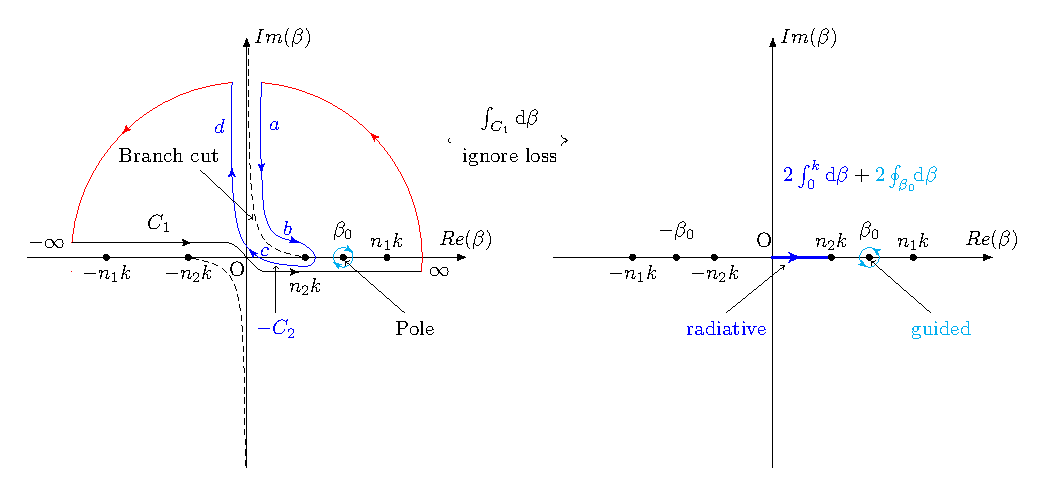
\includegraphics[scale=0.75]{../media/Figs/contourplot_upper}}
\end{minipage}
\par\medskip
\begin{minipage}{.91\linewidth}
\centering
\subfloat[]{\label{contourplot_lower}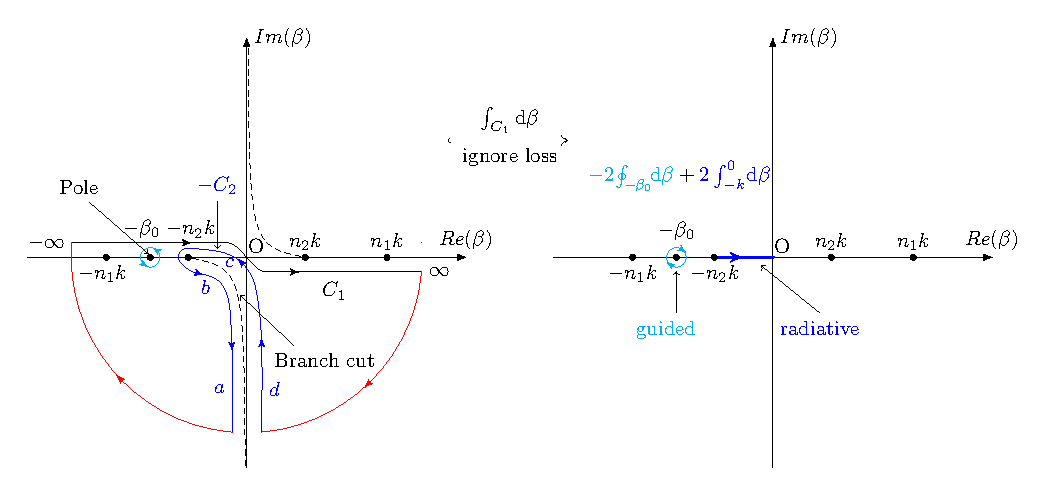
\includegraphics[scale=0.75]{../media/Figs/contourplot_lower}}
\end{minipage}
\caption[Contour integrations to decompose the guided and radiation modes of a dipole radiation problem in presence of a single mode waveguide.]{Integration paths. For the case that $ z>0 $, we can use the zero-valued contour integral path drawn in subfig.~\ref{contourplot_upper} to calculate the integration along path $ C_1 $. The simplified integration path by ignoring waveguide losses is given on the right-hand-side. It only contains the forward propagating mode contributions with radiation and guided mode components as divided through the real axis integral and the loop-hole integral. For the $ z<0 $ case, the contour integral analysis is given in subfig.~\ref{contourplot_lower}, which only includes the backward propagating mode contributions.}
\label{fig:integralpath}
\end{figure}

Now, we only consider the $ m=\pm 1 $ modes, and hence Equs.~(\ref{ET0Rexpand},~\ref{BT0Rexpand}) and the corresponding $ \phi $ and $ r\!_\perp $ components can be explicitly expressed as contour integrals
\begin{subequations}\label{ET0RC1}
\begin{align}
\mathcal{E}^{(T)}_z &= \sum_{m=\pm 1} \int_{C_1} \mathrm{d}\beta e^{im(\phi-\phi') + i\beta (z-z')} c_{m\beta} J_m (hr\!_\perp),\\
% + B_{m\beta} Y_m(hr\!_\perp)\right],\\
\mathcal{E}^{(0)}_{z} &= \sum_{m=\pm 1} \int_{C_1} \mathrm{d}\beta e^{im(\phi-\phi') + i\beta (z-z')} \mathcal{E}^{(0)}_{z,m\beta}(r\!_\perp)\\
\mathcal{E}^{(R)}_z &= \sum_{m=\pm 1} \int_{C_1} \mathrm{d}\beta e^{im(\phi-\phi') + i\beta (z-z')} a_{m\beta} H_m^{(1)} (pr\!_\perp),
\end{align}
\end{subequations}
\begin{subequations}\label{BT0RC1}
\begin{align}
\mathcal{B}^{(T)}_z &= \sum_{m=\pm 1} \int_{C_1} \mathrm{d}\beta e^{im(\phi-\phi') + i\beta (z-z')} d_{m\beta} J_m (hr\!_\perp),\\
% + E_{m\beta} Y_m(hr\!_\perp)\right],\\
\mathcal{B}^{(0)}_{z} &= \sum_{m=\pm 1} \int_{C_1} \mathrm{d}\beta e^{im(\phi-\phi') + i\beta (z-z')} \mathcal{B}^{(0)}_{z,m\beta}(r\!_\perp)\\
\mathcal{B}^{(R)}_z &= \sum_{m=\pm 1} \int_{C_1} \mathrm{d}\beta e^{im(\phi-\phi') + i\beta (z-z')} b_{m\beta} H_m^{(1)} (pr\!_\perp).
\end{align}
\end{subequations}
To distinguish the guided and radiation modes contributions, we can use the integral path along $ C_1 $ (see Fig.~\ref{fig:integralpath}) and find the equivalent integral path avoiding the branch cuts and isolated poles, which will be discussed next. 

For the free-dipole radiation components, the $ C_1 $ integral path is almost the real integral path from $ -\infty $ to the $ +\infty $ except for the branch point at $ \pm k $. The sign of $ \beta $ indicates the propagation direction of the field. The free-dipole components only yield the radiation mode contributions to the total Green's dyadic. This is because the dipole radiation only occurs outside of the fiber and always in the radiation potential zone according to the equivalent scattering potential model. 

For the reflection and transmission components of the field, there are poles in the $ a_{m\beta} $, $ b_{m\beta} $, $ c_{m\beta} $ and $ d_{m\beta} $ coefficients. There are also branch cuts hidden in the Bessel and Hankel function components of their expressions. Depending on the sign of $ (z-z') $, the integral paths and their simplification are shown in Fig.(\ref{fig:integralpath}). The guided modes are associated with poles, and hence can be represented as residues if asymptotic approximation can be made. Therefore, the guided mode contribution part of the reflection and transmission components can be given by
\begin{subequations}\label{ET0RRes}
\begin{align}
\mathcal{E}^{(T)}_z &= \sum_{m=\pm 1} \oint_{\beta_{1,m}}  e^{im(\phi\!-\!\phi') + i\beta (z\!-\!z')} c_{m\beta} J_m (hr\!_\perp),\\
%\mathcal{E}^{(0)}_{z} &= 2\pi i \sum_{m=\pm 1} \sum_{\beta_{1,m=\pm 1}}\mathrm{Res}\left[  e^{im(\phi-\phi') + i\beta (z-z')} \mathcal{E}^{(0)}_{z,m\beta}(r\!_\perp)\right]_{\beta=\beta_{1,m}},\\
\mathcal{E}^{(R)}_z &= \sum_{m=\pm 1} \oint_{\beta_{1,m}} e^{im(\phi\!-\!\phi') + i\beta (z\!-\!z')} a_{m\beta} H_m^{(1)} (pr\!_\perp),
\end{align}
\end{subequations}
\begin{subequations}\label{BT0RRes}
\begin{align}
\mathcal{B}^{(T)}_z &= \sum_{m=\pm 1} \oint_{\beta_{1,m}} e^{im(\phi\!-\!\phi') + i\beta (z\!-\!z')} d_{m\beta} J_m (hr\!_\perp),\\
%\mathcal{B}^{(0)}_{z} &= 2\pi i \sum_{m=\pm 1} \sum_{\beta_{1,m=\pm 1}}\mathrm{Res}\left[  e^{im(\phi-\phi') + i\beta (z-z')} \mathcal{B}^{(0)}_{z,m\beta}(r\!_\perp)\right]_{\beta=\beta_{1,m}}, \\
\mathcal{B}^{(R)}_z &= \sum_{m=\pm 1} \oint_{\beta_{1,m}} e^{im(\phi\!-\!\phi') + i\beta (z\!-\!z')} b_{m\beta} H_m^{(1)} (pr\!_\perp).
\end{align}
\end{subequations}
%\begin{subequations}\label{ET0RRes}
%\begin{align}
%\mathcal{E}^{(T)}_z &= 2\pi i \sum_{m=\pm 1} \sum_{\beta_{1,m=\pm 1}}\mathrm{Res}\left[  e^{im(\phi\!-\!\phi') + i\beta (z\!-\!z')} c_{m\beta} J_m (hr\!_\perp)\right]_{\beta=\beta_{1,m}},\\
%% + B_{m\beta} Y_m(hr\!_\perp)\right],\\
%\mathcal{E}^{(0)}_{z} &= 2\pi i \sum_{m=\pm 1} \sum_{\beta_{1,m=\pm 1}}\mathrm{Res}\left[  e^{im(\phi-\phi') + i\beta (z-z')} \mathcal{E}^{(0)}_{z,m\beta}(r\!_\perp)\right]_{\beta=\beta_{1,m}},\\
%\mathcal{E}^{(R)}_z &= 2\pi i \sum_{m=\pm 1} \sum_{\beta_{1,m=\pm 1}}\mathrm{Res}\left[ e^{im(\phi\!-\!\phi') + i\beta (z\!-\!z')} a_{m\beta} H_m^{(1)} (pr\!_\perp)\right]_{\beta=\beta_{1,m}},
%\end{align}
%\end{subequations}
%\begin{subequations}\label{BT0RRes}
%\begin{align}
%\mathcal{B}^{(T)}_z &= 2\pi i \sum_{m=\pm 1} \sum_{\beta_{1,m=\pm 1}}\mathrm{Res}\left[ e^{im(\phi\!-\!\phi') + i\beta (z\!-\!z')} d_{m\beta} J_m (hr\!_\perp)\right]_{\beta=\beta_{1,m}},\\
%% + E_{m\beta} Y_m(hr\!_\perp)\right],\\
%\mathcal{B}^{(0)}_{z} &= 2\pi i \sum_{m=\pm 1} \sum_{\beta_{1,m=\pm 1}}\mathrm{Res}\left[  e^{im(\phi-\phi') + i\beta (z-z')} \mathcal{B}^{(0)}_{z,m\beta}(r\!_\perp)\right]_{\beta=\beta_{1,m}}, \\
%\mathcal{B}^{(R)}_z &= 2\pi i \sum_{m=\pm 1} \sum_{\beta_{1,m=\pm 1}}\mathrm{Res}\left[ e^{im(\phi\!-\!\phi') + i\beta (z\!-\!z')} b_{m\beta} H_m^{(1)} (pr\!_\perp)\right]_{\beta=\beta_{1,m}}.
%\end{align}
%\end{subequations}

The radiation mode contributions of the reflection and transmission components are associated with the branch cuts $ C_2 $~\cite{Klimov2004} in Fig.(\ref{fig:integralpath}).
\begin{subequations}\label{ET0RC2}
\begin{align}
\mathcal{E}^{(T)}_z &= \sum_{m=\pm 1} \int_{C_2} \mathrm{d}\beta e^{im(\phi-\phi') + i\beta (z-z')} c_{m\beta} J_m (hr\!_\perp)\\
&\approx \sum_{m=\pm 1} 2\int_{-n_2k}^{n_2k} \mathrm{d}\beta e^{im(\phi-\phi') + i\beta (z-z')} c_{m\beta} J_m (hr\!_\perp),\\
%\mathcal{E}^{(0)}_{z} &= \sum_{m=\pm 1} \oint_{C_2} \mathrm{d}\beta e^{im(\phi-\phi') + i\beta (z-z')} \mathcal{E}^{(0)}_{z,m\beta}(r\!_\perp),\\
\mathcal{E}^{(R)}_z &= \sum_{m=\pm 1} \oint_{C_2} \mathrm{d}\beta e^{im(\phi-\phi') + i\beta (z-z')} a_{m\beta} H_m^{(1)} (pr\!_\perp)\\
&\approx \sum_{m=\pm 1} 2\int_{-n_2k}^{n_2k} \mathrm{d}\beta e^{im(\phi-\phi') + i\beta (z-z')} a_{m\beta} H_m^{(1)} (pr\!_\perp),
\end{align}
\end{subequations}
\begin{subequations}\label{BT0RC2}
\begin{align}
\mathcal{B}^{(T)}_z &= \sum_{m=\pm 1} \oint_{C_2} \mathrm{d}\beta e^{im(\phi-\phi') + i\beta (z-z')} d_{m\beta} J_m (hr\!_\perp)\\
&\approx \sum_{m=\pm 1} 2\int_{-n_2k}^{n_2k} \mathrm{d}\beta e^{im(\phi-\phi') + i\beta (z-z')} d_{m\beta} J_m (hr\!_\perp),\\
%\mathcal{B}^{(0)}_{z} &= \sum_{m=\pm 1} \oint_{C_2} \mathrm{d}\beta e^{im(\phi-\phi') + i\beta (z-z')} \mathcal{B}^{(0)}_{z,m\beta}(r\!_\perp),\\
\mathcal{B}^{(R)}_z &= \sum_{m=\pm 1} \oint_{C_2} \mathrm{d}\beta e^{im(\phi-\phi') + i\beta (z-z')} b_{m\beta} H_m^{(1)} (pr\!_\perp)\\
&\approx \sum_{m=\pm 1} 2\int_{-n_2k}^{n_2k} \mathrm{d}\beta e^{im(\phi-\phi') + i\beta (z-z')} b_{m\beta} H_m^{(1)} (pr\!_\perp).
\end{align}
\end{subequations}
Above, the approximation works when the waveguide is lossless and hence the branch lines along the imaginary axis of the $ \beta $ plane can be ignored. The factor of $ 2 $ comes from the sign flip of the two branch lines parallel to the real axis in the $ \beta $ plane ($ 2=1-\mathrm{e}^{\pi i} $), and physically corresponds to the degeneracy of $ 2 $ degrees of freedom of the polarization of the radiation modes in the transverse plane. Although we use the integral limits $ -n_2k $ to $ n_2k $, in practice, it should be either $ 0 \rightarrow n_2k$ or $ -n_2k\rightarrow 0 $ depending on the propagation directions of interest. 

One can obtain the bound and radiation field components with the dipole oriented in $ z $, $ \phi $ and $ r\!_\perp $ directions by substituting the $ \bmc{E}^{(0)}_{m\beta}(r\!_\perp) $ expressions for corresponding cases into Eqs.~(\ref{ET0RRes}-\ref{BT0RC2}). 

To calculate the guided modes, we need to calculate the residues at isolated poles with $ \beta_{1,m} $ and $ m=\pm 1 $. The poles can be found by using the condition that
\begin{align}
D=P^2+QR=0,
\end{align}
or
\begin{align}\label{pole4beta}
&\beta^2m^2k^4\left[J_m(ha) H_m^{(1)}(pa) \right]^2 (\varepsilon_f-1)^2\nonumber\\
-& h^2p^2a^2k^2 \left[hJ_m(ha) \dd{}{(pa)}H_m^{(1)}(pa)-pH_m^{(1)}(pa)\dd{}{(ha)}J_m(ha) \right]\nonumber\\ &\times\left[hJ_m(ha) \dd{}{(pa)}H_m^{(1)}(pa)-\varepsilon_f pH_m^{(1)}(pa)\dd{}{(ha)}J_m(ha) \right]=0.
\end{align}
Useful relationships to solve the equation above are
\begin{align}
J_{-m}(z)=(-1)^nJ_n(z),\, &\quad H_{-m}^{(1)}(z)=e^{m\pi i}H_m^{(1)}(z),\\
\dd{}{z}J_m(z) &= \frac{1}{2} \left( J_{m-1}(z)-J_{m+1}(z) \right),\\ 
\dd{}{z}H^{(1)}_m(z) &= \frac{1}{2} \left( H^{(1)}_{m-1}(z)-H^{(1)}_{m+1}(z) \right).
\end{align}
We can rewrite Eq.~(\ref{pole4beta}) as
\begin{align}\label{pole4beta2}
&\beta^2m^2k^2\left(J_m\!(ha) H_m^{(\!1\!)}\!(pa) \right)^2 (\varepsilon_f-1)^2\nonumber\\
=& \frac{h^2p^2a^2}{4} \left[hJ_m\!(ha)\! \left( H^{(\!1\!)}_{m-1}\!(pa)\!-\! H^{(\!1\!)}_{m+1}\!(pa) \right)\!-\! pH_m^{(\!1\!)}\!(pa)\left( J_{m-1}\!(ha)\!-\! J_{m+1}\!(ha) \right) \right]\nonumber\\ 
&\!\!\!\!\times\!\left[ \! hJ_m\!(ha)\! \left(\! H^{(\!1\!)}_{m-1}\!(pa)\!-\! H^{(\!1\!)}_{m+1}\!(pa)\! \right)\!-\! \varepsilon_f pH_m^{(\!1\!)}\!(pa)\!\left( J_{m-1}\!(ha)\!-\! J_{m+1}\!(ha) \right) \right]\!.
\end{align}
Since both $ h $ and $ p $ are functions of $ \beta $, the equation above is complicated in solving for $ \beta $. If $ ka<0.8 $, asymptotic approximation is good enough to solve Eq.~(\ref{pole4beta2}) and gives an analytic solution for $ \beta $~\cite{Klimov2004}. However, in our nanofiber case, this $ ka<0.8 $ condition is not satisfied. We should be able to numerically solve Eq.~(\ref{pole4beta2}) for $ \beta $ as the characteristic constant for the guided mode with $ m=\pm 1 $. %\textcolor{red}{Q: we may be able to prove that Eq.~\eqref{pole4beta2} is equivalent to the eigen equation of $ \beta $ for the bare fiber case. Useful relationship: $ K_n(x)=\frac{\pi}{2}i^{n+1}H_n^{(1)}(ix) $.}

Numerically, the $ \beta_0 $ solved from the radiation problem is indistinguishable with the one solved from the nanofiber's eigenmode equation in the regime we are interested in.

Next, we solve for the guided modes contributions to the longitudinal components of the fields by applying the residual theorem to Eqs.~\eqref{ET0RRes} and~\eqref{BT0RRes} and differentiating the denominator that generates poles evaluated at $ \beta_{1,m=\pm 1} $. %\textcolor{red}{(Q: are those poles all of order 1?)} 
All transverse components of the fields can be obtained from the longitudinal components using the relations of Eq.~\ref{EHzgauss}. 
%Sample numerical calculations has been performed, and results are documented in the NanofiberProjectPlots.pdf (Dropbox folder, \url{Nanofiber/Code/Matlab/Plots}). The primary plots show that there are phase shifts for the transmitted and reflected lights so that the mode profile is not symmetric to the $ x $ axis where the atom lies on; the reflected light field has a backaction on the atom tending to move it off the trapping point; the $ m=\pm 1 $ modes are not balanced... 
Our results were checked by reproducing the decay rates provided in Ref.~\cite{Klimov2004}. 

To calculate the total decay rate of the atom with the enhancement due to the radiation, we need to find out the functions describing the branch cuts and the integration path for the radiation modes. The equations defining the branch cut are given by
\begin{align}\label{branchcutequ}
\mathrm{Im}\left[p \right] &=0\\
\mathrm{Im}\left[h\right] &=0.
\end{align}
By setting $ \beta=x+iy $, we can rewrite the first equation as
\begin{align}
p&=\sqrt{k^2-\beta^2}\\
&=\left[(k^2-x^2+y^2)^2 + 4x^2y^2 \right]^{1/4}e^{\frac{i}{2}\arctan\frac{-2xy}{k^2-x^2+y^2}}.
\end{align}
Hence Eq.~(\ref{branchcutequ}) yields
\begin{align}
0&= \left[(k^2-x^2+y^2)^2 + 4x^2y^2 \right]^{1/4} \sin \left[\frac{1}{2}\arctan\frac{-2xy}{k^2-x^2+y^2} \right]\\
&= \frac{1}{\sqrt{2}} \left[(k^2\!-\! x^2\!+\! y^2)^2 \!+\! 4x^2y^2 \right]^{1/4} \sqrt{1\!-\!\cos \left(\arctan\frac{-2xy}{k^2\!-\! x^2\!+\! y^2} \right)}\\
&= \frac{1}{\sqrt{2}} \left[(k^2\!-\!x^2\!+\! y^2)^2 \!+\! 4x^2y^2 \right]^{1/4} \sqrt{1\!-\! \frac{k^2\!-\! x^2\!+\! y^2}{\left[(k^2\!-\! x^2\!+\! y^2)^2 \!+\! 4x^2y^2 \right]^{1/2}} }\\
&=\sqrt{\left[(k^2-x^2+y^2)^2 + 4x^2y^2 \right]^{1/2}-(k^2-x^2+y^2)},
\end{align}
which gives
\begin{align}
\left[(k^2-x^2+y^2)^2 + 4x^2y^2 \right]^{1/2}&=(k^2-x^2+y^2),\\
\Leftrightarrow \qquad \qquad \qquad \qquad \qquad x^2y^2&=0.\label{branchcut2}
\end{align}
Obviously, the $ x $ axis between $ [-k,k] $ and the entire $ y $ axis are the branch cuts. To separate the branches into upper and lower parts, we can define an arbitrarily small positive number $ \delta\epsilon\rightarrow 0 $ so that Eq.~\eqref{branchcut2} gives
\begin{align}
xy&=\delta\epsilon.
\end{align}
Similarly, the condition for $ \mathrm{Im}[h]=0 $ gives the same result. To make the field components homomorphic at any point in the complex $ \beta $ plane, we choose the branch cuts that satisfy 
\begin{align}
xy&>\delta\epsilon>0.
\end{align}
By the physics condition of radiation mode, we also have 
\begin{align}
-n_2k<x<n_2k.
\end{align}
In this way, the branch cuts as hyperbola-type lines are symmetrically separated into top-right and lower-left parts, and are very close to the $ x- $ and $ y- $ axes. 
For the top-right branch, one can choose the integration path as shown in Fig.~\ref{fig:integralpath} in the contour integral avoiding the branch cut. 

%\scalefig{Figs/contourpath2}{0.8}{Integration path of the contour integral for radiation modes.}

In the case where the nanofiber can be treated as a lossless medium, the contour integral can be treated as an integral over real axis from $ -kn_2 $ to $ kn_2 $. 
We illustrate the division of the guided and unguided mode contributions to the integration over $ \beta $ in Fig.~\ref{fig:integralpaths} and show the contour integrals in different regions to be calculated. 

\begin{figure}[!tbp]
\centering\makebox[\textwidth]{
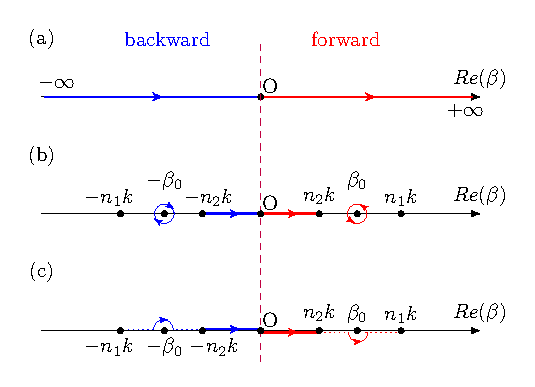
\includegraphics[width=0.85\textwidth]{../media/Figs/integratepath_GF}}
\caption[Integral paths for the dyadic Green's function calculations when loss is negligible.]{Integral paths for the dyadic Green's function calculations. Part (a) is the integral path for the dipole's free-space field contribution calculation [see, for example, Eq.~\eqref{ET0RC1}]. Part (b) is the integral path for the reflected and transmitted field contributions calculation [see, for example, Eq.~\eqref{ET0RC1}]. Part (c) is the integral path for the dyadic Green's function calculation using the eigenmode decomposition method [see Eqs.~\eqref{Eq::GreensEigenmodes} and~\eqref{Eq::GreensunguidedEigenmodes}]. The integral paths on the left-hand-side (in blue) indicate the backward propagating contributions, while the right-hand-side (in red) parts corresponding to the forward propagating contributions. For the eigenmode decomposition method in part (c), if one choose to use $ f=\pm 1 $ to indicate the propagation direction, then only the $ \beta>0 $ portion of integral path will be applied. }
\label{fig:integralpaths}
\end{figure}

As shown in section~\ref{sec:eigenmodesofwaveguides}, the guided and radiation modes contribution to the dyadic Green's function can be identified through the specific choice of integral paths. Fig.~\ref{fig:integralpaths}, part (a) shows the integral path to calculate the dipole free-space contribution which does not yield guided mode contribution to the total dyadic Green's function. Part (b) shows the loop and real-valued integral paths of the guided and radiation mode-divisions to the reflected and transmitted field components. The $ \mathrm{Re}(\beta)<0 $ and $ \mathrm{Re}(\beta)>0 $ parts correspond to the backward and forward propagating contributions, respectively. Part (c) of the figure indicates the path using the eigenmode decomposition method in the case where the sign of $ \mathrm{Re}(\beta) $ indicates the propagation directions. Depending on the propagation directions, we should choose the right integral paths for the corresponding methods adopted, and different methods should yield the same result. 


With all of the field components solved given a dipole vector, the dyadic Green's function can be calculated with three parts: the part due to free-dipole radiation, $ \GFT_0(\br,\br') $, the field reflection part due to the presence of the waveguide interface, $ \GFT_R(\br,\br') $, and the part due to mode transmission through the waveguide, $ \GFT_T(\br,\br') $. The former two parts generate the unguided mode contribution to the total dyadic Green's function, and the third part forms the guided mode contribution to the total dyadic Green's function. The $ ij $-th components of the three parts of the dyadic Green's function can then be calculated by (see Eq.~\eqref{eq:GFTijEd})
\begin{align}
G_0^{ij}(\br,\br') &= \frac{\mathcal{E}_i^{(0)}(\br)}{d_j(\br')},\\
G_R^{ij}(\br,\br') &= \frac{\mathcal{E}_i^{(R)}(\br)}{d_j(\br')},\\
G_T^{ij}(\br,\br') &= \frac{\mathcal{E}_i^{(T)}(\br)}{d_j(\br')},
\end{align}
where $ \mathcal{E}_i^{(A)}\,(A=0,R,T) $ are the $ i $-th free-dipole radiation, and interface reflection and mode transmission electric components due to the corresponding dipole $ d_j $ orientated along the $ \mathbf{e}_j $ direction. The total dyadic Green's function is
\begin{align}
\GFT(\br,\br')=\GFT_0(\br,\br')+\GFT_R(\br,\br')+\GFT_T(\br,\br') .
\end{align} 


%</nanofiberradiationproblem>


%<*choozingSWGs>
\chapter{The choice of square waveguides for this study}\label{chap:choozingSWGs}
\section{Phase walkoff problems of rectangular waveguides}
Based on the enhanced QND-measurement--induced spin squeezing protocol we have studied in Ref.~\cite{Qi2017Enhanced} or Chapter~\ref{chap:Faraday}, a key to generate a strong spin squeezing effect for QND measurement is to find orthogonal modes that couple the ``local oscillator" and the ``signal". 
We can denote them as $ H $ and $ V $ modes. 
In general, the field operator for the QND measurement can be written as 
\begin{align}\label{eq:EdifferentHV}
\hat{\mathbf{E}}^{(+)}(r\!_\perp,\phi,z;t) &= \sqrt{ \frac{2 \pi \hbar \omega_0}{ v_g^H} } \mathbf{u}_H(r\!_\perp,\phi) \hat{a}_H(z,t)  e^{i (\beta_0^H z- \omega_0 t)}\nn\\
&\quad +\sqrt{ \frac{2 \pi \hbar \omega_0}{ v_g^V} } \mathbf{u}_V(r\!_\perp,\phi) \hat{a}_V(z,t)  e^{i (\beta_0^V z- \omega_0 t)},
\end{align}
where $ v_g^{H/V} $ and $ \beta_0^{H/V} $ are the group velocities and propagation constants of the $ H $ and $ V $ modes, respectively. When a rectangular waveguide is used, $ v_g^H $ and $ v_g^V $, so as the projected mode constants $ \beta_0^H $ and $ \beta_0^V $, become non-degenerate.
The offset of $ v_g^{H/V} $ and $ \beta_0^{H/V} $ between the two guided modes could lead to a walkoff effect and causes an intrinsic phase shift.
We want to avoid this walkoff effect, unless the phase shift between the two modes at atom positions are multiples of $ 2\pi $, which is difficult to implement as we will show next. 
%This follows discussions held with the collaborators on Ref.~\cite{Qi2017Enhanced}.

\section{Optimal width of a \SWG to tolerate fabrication imperfections}

Four plots shown in Fig.~\ref{fig:ng_rect_dwg} are the phase and group indices of refractions of general rectangular waveguides in determining the
preferred waveguie size for our study. 
%I made four plots when I and Dr. Jongmin Lee were working on determining the preferable dimension of the waveguides. See Fig.~\ref{fig:ng_rect_dwg}.

\begin{figure}[!tbp]
\centering
\begin{minipage}[h]{\linewidth}
 %\begin{tabular}{*{2}{b{0.2\textwidth-2\tabcolsep}}}
  \subfloat[h][]{
    %% This file was created by matlab2tikz.
%
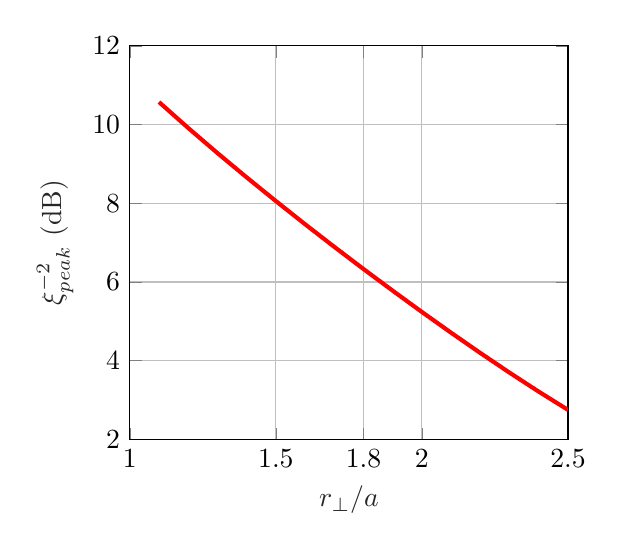
\begin{tikzpicture}

\begin{axis}[%
width=5.565cm,
height=5cm,
at={(0cm,0cm)},
scale only axis,
xmin=1.0000,
xmax=2.5000,
xtick={1.0000,1.5000,1.8000,2.0000,2.5000},
xlabel style={font=\color{white!15!black}},
xlabel={$r_\perp/a$},
ymin=2.0000,
ymax=12.0000,
ylabel style={font=\color{white!15!black}},
ylabel={$\xi^{-2}_{peak}$ (dB)},
axis background/.style={fill=white},
xmajorgrids,
ymajorgrids
]
\addplot [color=red, line width=1.5pt, forget plot]
  table[row sep=crcr]{%
1.1000	10.5712\\
1.2000	9.9128\\
1.3000	9.2762\\
1.4000	8.6588\\
1.5000	8.0571\\
1.6000	7.4685\\
1.7000	6.8935\\
1.8000	6.3307\\
1.9000	5.7799\\
2.0000	5.2394\\
2.1000	4.7118\\
2.2000	4.1974\\
2.3000	3.6980\\
2.4000	3.2157\\
2.5000	2.7531\\
};
\end{axis}
\end{tikzpicture}%
    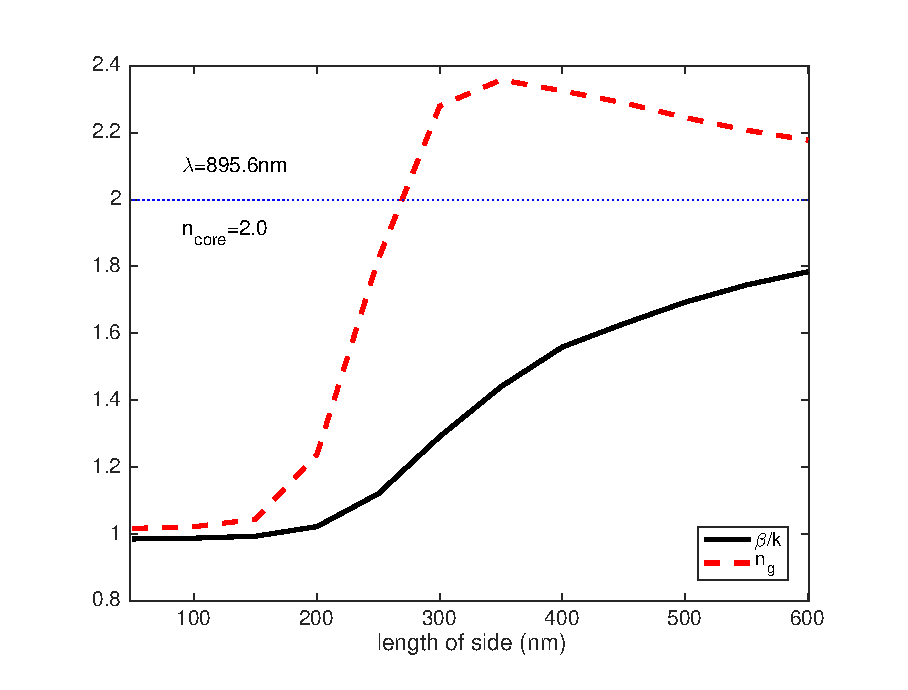
\includegraphics[width=0.48\linewidth]{../media/Figs/ng_D1_dwg}
    \label{fig:ng_D1_dwg}
    }
    \hfill
  \subfloat[h][]{
      \label{fig:ng_D2_dwg}
      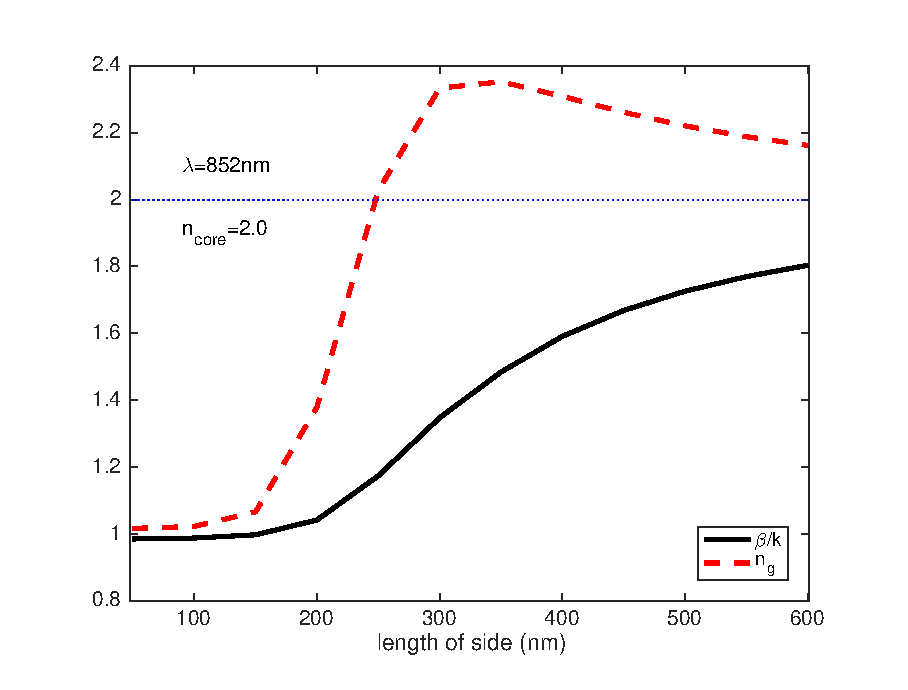
\includegraphics[width=0.48\linewidth]{../media/Figs/ng_D2_dwg}
      %% This file was created by matlab2tikz.
%
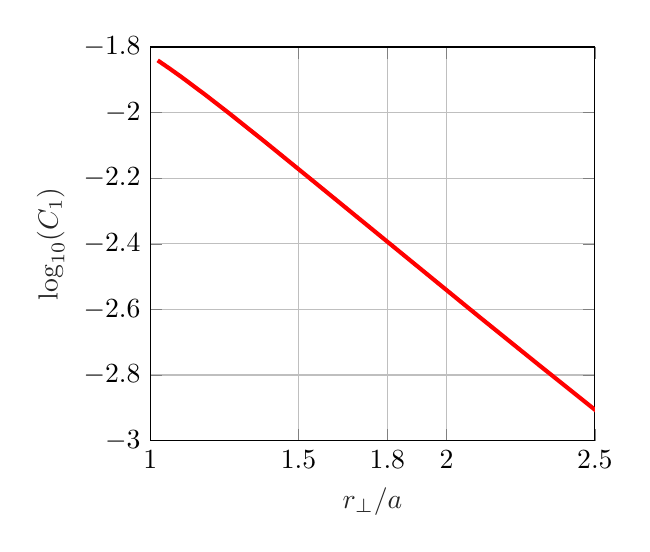
\begin{tikzpicture}

\begin{axis}[%
width=5.647cm,
height=5cm,
at={(0cm,0cm)},
scale only axis,
xmin=1.0000,
xmax=2.5000,
xtick={1.0000,1.5000,1.8000,2.0000,2.5000},
xlabel style={font=\color{white!15!black}},
xlabel={$r_\perp/a$},
ymin=-3.0000,
ymax=-1.8000,
ylabel style={font=\color{white!15!black}},
ylabel={$\log_{10}(C_1)$},
axis background/.style={fill=white},
xmajorgrids,
ymajorgrids
]
\addplot [color=red, line width=1.5pt, forget plot]
  table[row sep=crcr]{%
1.0251	-1.8409\\
1.0653	-1.8658\\
1.1055	-1.8917\\
1.1859	-1.9459\\
1.2663	-2.0022\\
1.3869	-2.0891\\
1.5477	-2.2073\\
2.1106	-2.6230\\
2.3116	-2.7696\\
2.5126	-2.9148\\
};
\end{axis}
\end{tikzpicture}%
      }
   \end{minipage}\vfill
   \begin{minipage}[h]{\linewidth}
    %\begin{tabular}{*{2}{b{0.2\textwidth-2\tabcolsep}}}
     \subfloat[h][]{
       %\input{fig/square waveguide_peakxi_rp_NA2500.tex}
       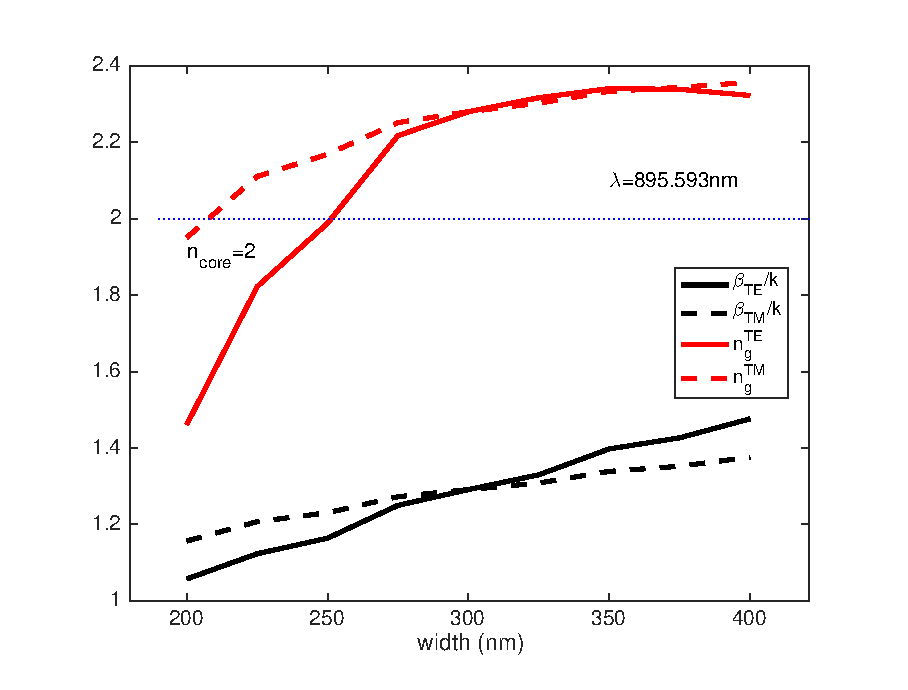
\includegraphics[width=0.48\linewidth]{../media/Figs/ng_D1_rectwg_dwg}
       \label{fig:ng_D1_rectwg_dwg}
       }
       \hfill
     \subfloat[h][]{
         \label{fig:ng_D2_rectwg_dwg}
         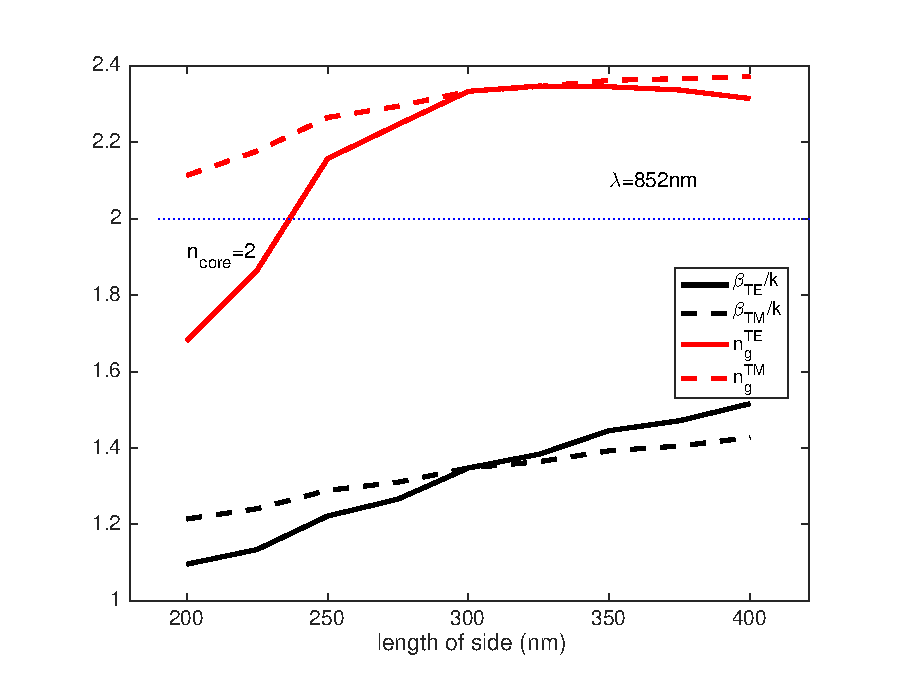
\includegraphics[width=0.48\linewidth]{../media/Figs/ng_D2_rectwg_dwg}
         %\input{fig/square waveguide_C1_y.tex}
         }
   \end{minipage}
\caption[Optimal choice of waveguide width to tolerate fabrication imperfections.]{Group index of refraction with changing width of a square waveguide ($ n_1=2.0,\,w=300 $ nm) at cesium's D1 line (a) and D2 line (b). Group indices of refraction and the phase indices of refraction\index{phase index of refraction} for the fundamental quasi-\TE and quasi-\TM modes of an imperfect \SWG with a side changing its length ($ x $ axis) at the D1 line (c) and the D2 line (d).}\label{fig:ng_rect_dwg}
\end{figure}

In the figure, (a) and (b) show that the group index of refraction\index{group index of refraction} $n_g$ reaches the
peak value at $\sim 300$ nm for both D1 line (a) and D2 line (b). The plateaus
at the $300$ nm $x$-axis value of the $n_g$ curves as a function
of the width of a square waveguide, indicating that $n_g$ will be the most
robust case in presence of fabrication fluctuations. 1\% of fabrication
imperfection may not be a big issue to worry about in our case.

In Fig.~\ref{fig:ng_rect_dwg}, (c) and (d), one side of the waveguide is fixed at $300$ nm while
varying the other side from $200$ nm to $400$ nm. The the phase index
of refraction ($\beta/k$) and the group index of fraction\index{group index of refraction} ($n_g$) for the
non-degenerate fundamental quasi-\TE and quasi-\TM modes are plotted. Our formulas of
effective mode areas for spin squeezing should be modified for the
non-degenerate mode case. We merely give the followling brief outline for the modification here: the $n_g$ in the formula of the effective interaction mode area for our Faraday spin squeezing protocol~\cite{Qi2017Enhanced}, $A_{\rm Far}$, should be replaced with the geometric average of $n_g^{TE}$ and $n_g^{TM}$, that is $\sqrt{n_g^{V} \times n_g^{H}}$ when $V$ and $H$ modes are the quasi-\TE and quasi-\TM modes; the equation for the  input mode area, $A_0$, maintains its original form. In the end,
the cooperavity formula should be modified by a factor of the square
root of the ratio between $n_g^V$ and $n_g^H$, where the input probe is
polarized along the $H$ direction and atoms are trapped on the $V$ axis.
From the plots of (c) and (d) at D1 and D2 lines, it is seen that the
phase indices of refraction are only barely distinguishable between the two modes with
$10\%/k$ maximum when one side of the waveguide is $200$ nm. The phase
matching condition basically tells us that the two groups of atoms
should be trapped in a minimum distance of $10\times k$, which might be too long to implement considering the great photon loss through the waveguide. Notice that the phase
difference between the two modes scales almost linearly when one side of
the waveguide decreases.

On the other hand, the ratio between the two group indices increases
dramatically when one side of the waveguide is shortened. But when we
plug in the numbers, with a $200$ nm $\times$ $300$ nm waveguide, the enhancement of
cooperativity is only about $15\%$ from the $300$ nm $\times$ $300$ nm square waveguide case. 
Considering that the trapping potential well gets sharper when the
corresponding side of the waveguide decreases, we think the most
important benefit of using a rectangular waveguide would be the ability
to make the trapping potential sharp on the direction parallel to the
nearest side of the waveguide. 
%\satomi{Qi, you probably don't have to say this following sentence.} We haven't considered the quantized trapping potential-level splitting on the vertical direction, which would be interesting for the experiment.

Regarding the phase mismatch issue, as along as the group velocities
do not make the light pulses of the two modes walk off in the
waveguide range significantly, the measurement signal with the time integral under a
resolution of ns or even longer won't distinguish the difference between the
signals of polarization states from the two groups of atoms. 
Since the birefringence rotation due to the mode distortion is deterministic given the number of atoms, we might be able to compensate for the phase drafting and extract the pure Faraday rotation from the measurement records.

%</choozingSWGs>

%###################################################################################
\bibliographystyle{../styles/abbrv-alpha-letters-links}
\bibliography{../refs/Archive}
%%%%%%%%%%%%%%%%%%%%%%%%%%%%%%%%%%%%%%%%%%%%%%%%%%%%%%%%%%%%%%%%%%%%%%%%%%%%%%%%%%%%

\printindex
\end{document}
